%%% Hlavní soubor. Zde se definují základní parametry a odkazuje se na ostatní části. %%%

%% Verze pro jednostranný tisk:
% Okraje: levý 40mm, pravý 25mm, horní a dolní 25mm
% (ale pozor, LaTeX si sám přidává 1in)
\documentclass[12pt,a4paper]{report}
\setlength\textwidth{145mm}
\setlength\textheight{247mm}
\setlength\oddsidemargin{15mm}
\setlength\evensidemargin{15mm}
\setlength\topmargin{0mm}
\setlength\headsep{0mm}
\setlength\headheight{0mm}
% \openright zařídí, aby následující text začínal na pravé straně knihy
\let\openright=\clearpage

%% Pokud tiskneme oboustranně:
% \documentclass[12pt,a4paper,twoside,openright]{report}
% \setlength\textwidth{145mm}
% \setlength\textheight{247mm}
% \setlength\oddsidemargin{14.2mm}
% \setlength\evensidemargin{0mm}
% \setlength\topmargin{0mm}
% \setlength\headsep{0mm}
% \setlength\headheight{0mm}
% \let\openright=\cleardoublepage

%% Vytváříme PDF/A-2u
\usepackage[a-2u]{pdfx}

%% Přepneme na českou sazbu a fonty Latin Modern
\usepackage[czech]{babel}
\usepackage{lmodern}
\usepackage[T1]{fontenc}
\usepackage{textcomp}

%% Použité kódování znaků: obvykle latin2, cp1250 nebo utf8:
\usepackage[utf8]{inputenc}

%%% Další užitečné balíčky (jsou součástí běžných distribucí LaTeXu)
\usepackage{amsmath}        % rozšíření pro sazbu matematiky
\usepackage{amsfonts}       % matematické fonty
\usepackage{amsthm}         % sazba vět, definic apod.
\usepackage{bbding}         % balíček s nejrůznějšími symboly
			    % (čtverečky, hvězdičky, tužtičky, nůžtičky, ...)
\usepackage{bm}             % tučné symboly (příkaz \bm)
\usepackage{graphicx}       % vkládání obrázků
\usepackage{fancyvrb}       % vylepšené prostředí pro strojové písmo
\usepackage{indentfirst}    % zavede odsazení 1. odstavce kapitoly
\usepackage[numbers]{natbib}         % zajištuje možnost odkazovat na literaturu
			    % stylem AUTOR (ROK), resp. AUTOR [ČÍSLO]
\usepackage[nottoc]{tocbibind} % zajistí přidání seznamu literatury,
                            % obrázků a tabulek do obsahu
\usepackage{icomma}         % inteligetní čárka v matematickém módu
\usepackage{dcolumn}        % lepší zarovnání sloupců v tabulkách
\usepackage{booktabs}       % lepší vodorovné linky v tabulkách
\usepackage{paralist}       % lepší enumerate a itemize
\usepackage{xcolor}         % barevná sazba
% Custom packages
\usepackage{tcolorbox}
\usepackage{float}
\usepackage{enumitem,amssymb}
\usepackage{tikz}
\usepackage{tabularx}
% load hyperref last
\usepackage{hyperref}       % odkazy

% List with square bullets
\newlist{todolist}{itemize}{2}
\setlist[todolist]{label=$\square$}

%%% Údaje o práci

% Název práce v jazyce práce (přesně podle zadání)
\def\NazevPrace{Platforma pro monitorování mentálního zdraví}

% Název práce v angličtině
\def\NazevPraceEN{Mental health monitoring platform}

% Jméno autora
\def\AutorPrace{Patrik Trefil}

% Rok odevzdání
\def\RokOdevzdani{2023}

% Název katedry nebo ústavu, kde byla práce oficiálně zadána
% (dle Organizační struktury MFF UK, případně plný název pracoviště mimo MFF)
\def\Katedra{Katedra softwarového inženýrství (204. • 32-KSI)}
\def\KatedraEN{Department of Software Engineering}

% Jedná se o katedru (department) nebo o ústav (institute)?
\def\TypPracoviste{Katedra softwarového inženýrství (204. • 32-KSI)}
\def\TypPracovisteEN{Department of Software Engineering}

% Vedoucí práce: Jméno a příjmení s~tituly
\def\Vedouci{Mgr. Petr Škoda, Ph.D.}

% Pracoviště vedoucího (opět dle Organizační struktury MFF)
\def\KatedraVedouciho{Katedra softwarového inženýrství (204. • 32-KSI)}
\def\KatedraVedoucihoEN{Department of Software Engineering}

% Studijní program a obor
\def\StudijniProgram{Informatika (B0613A140006)}
\def\StudijniObor{IPP2 (0613RA1400060006)}

% Nepovinné poděkování (vedoucímu práce, konzultantovi, tomu, kdo
% zapůjčil software, literaturu apod.)
\def\Podekovani{%
    Chtěl bych vyjádřit svou vděčnost mé přítelkyni za její podporu a trpělivost, mojí rodině a přátelům za jejich povzbuzení a cenné rady v průběhu mého studia.
    Velké díky patří také mému vedoucímu práce Mgr.\ Petru Škodovi,\ Ph.D., jehož odborné vedení a cenné připomínky byly pro mě velkým přínosem.
    Díky vám všem za to, že jste byli součástí této cesty.
}

% Abstrakt (doporučený rozsah cca 80-200 slov; nejedná se o zadání práce)
%% Nezapomeňte upravit abstrakt.xmpdata.

\def\Abstrakt{%
    V Národním ústavu duševního zdraví vznikla potřeba pro digitalizaci výzkumné a terapeutické praxe.
    Jedním z procesů k digitalizaci byla spolupráce terapeutů s pacienty/klienty formou dotazníků.
    V rámci práce byla provedena analýza, návrh a implementace webové aplikace digitalizující tento proces.
    Aplikace umožňuje tvorbu a zpracování dotazníků.
    Tuto funkcionalitu lze použít i pro sběr dat pro výzkumné účely.
    Mezi hlavní kvalitativní požadavky ústavu patřila snadná rozšiřitelnost aplikace o další formy spolupráce a možnost provozu aplikace na vlastní infrastruktuře.
    Tyto požadavky byly adresovány vhodným rozdělením aplikace na komponenty a využití Docker pro snadné nasazení.
    Aplikace byla úspěšně předána ústavu k nasazení.
}

\def\AbstraktEN{%
    The National Institute of Mental Health needed to digitalize its research and therapeutic practice. % TODO: reflect changes from the Czech version
    This thesis deals with the development of a web platform that provides therapists with tools for collaborating with patients and clients outside of regular therapeutic sessions.
    Within this work, collaboration in the form of questionnaires was implemented.
    This functionality can also be used for data collection for research purposes.
    The application was designed for easy extension with additional forms of collaboration.
    The application is prepared for the improvement of the provided care and was successfully delivered to the client.
}


% 3 až 5 klíčových slov (doporučeno), každé uzavřeno ve složených závorkách
\def\KlicovaSlova{%
{vývoj software}, {webová aplikace}, {formuláře}
}
\def\KlicovaSlovaEN{%
{software development}, {web application}, {forms}
}

%% Balíček hyperref, kterým jdou vyrábět klikací odkazy v PDF,
%% ale hlavně ho používáme k uložení metadat do PDF (včetně obsahu).
%% Většinu nastavítek přednastaví balíček pdfx.
\hypersetup{unicode}
\hypersetup{breaklinks=true}

%% Definice různých užitečných maker (viz popis uvnitř souboru)
%%% Tento soubor obsahuje definice různých užitečných maker a prostředí %%%
%%% Další makra připisujte sem, ať nepřekáží v ostatních souborech.     %%%

%%% Drobné úpravy stylu

% Tato makra přesvědčují mírně ošklivým trikem LaTeX, aby hlavičky kapitol
% sázel příčetněji a nevynechával nad nimi spoustu místa. Směle ignorujte.
\makeatletter
\def\@makechapterhead#1{
  {\parindent \z@ \raggedright \normalfont
   \Huge\bfseries \thechapter. #1
   \par\nobreak
   \vskip 20\p@
}}
\def\@makeschapterhead#1{
  {\parindent \z@ \raggedright \normalfont
   \Huge\bfseries #1
   \par\nobreak
   \vskip 20\p@
}}
\makeatother

% Toto makro definuje kapitolu, která není očíslovaná, ale je uvedena v obsahu.
\def\chapwithtoc#1{
\chapter*{#1}
\addcontentsline{toc}{chapter}{#1}
}

% Trochu volnější nastavení dělení slov, než je default.
\lefthyphenmin=2
\righthyphenmin=2

% Zapne černé "slimáky" na koncích řádků, které přetekly, abychom si
% jich lépe všimli.
\overfullrule=1mm

%%% Makra pro definice, věty, tvrzení, příklady, ... (vyžaduje baliček amsthm)

\theoremstyle{plain}
\newtheorem{veta}{Věta}
\newtheorem{lemma}[veta]{Lemma}
\newtheorem{tvrz}[veta]{Tvrzení}

\theoremstyle{plain}
\newtheorem{definice}{Definice}

\theoremstyle{remark}
\newtheorem*{dusl}{Důsledek}
\newtheorem*{pozn}{Poznámka}
\newtheorem*{prikl}{Příklad}

%%% Prostředí pro důkazy

\newenvironment{dukaz}{
  \par\medskip\noindent
  \textit{Důkaz}.
}{
\newline
\rightline{$\qedsymbol$}
}

%%% Prostředí pro sazbu kódu, případně vstupu/výstupu počítačových
%%% programů. (Vyžaduje balíček fancyvrb -- fancy verbatim.)

\DefineVerbatimEnvironment{code}{Verbatim}{fontsize=\small, frame=single}

%%% Prostor reálných, resp. přirozených čísel
\newcommand{\R}{\mathbb{R}}
\newcommand{\N}{\mathbb{N}}

%%% Užitečné operátory pro statistiku a pravděpodobnost
\DeclareMathOperator{\pr}{\textsf{P}}
\DeclareMathOperator{\E}{\textsf{E}\,}
\DeclareMathOperator{\var}{\textrm{var}}
\DeclareMathOperator{\sd}{\textrm{sd}}

%%% Příkaz pro transpozici vektoru/matice
\newcommand{\T}[1]{#1^\top}

%%% Vychytávky pro matematiku
\newcommand{\goto}{\rightarrow}
\newcommand{\gotop}{\stackrel{P}{\longrightarrow}}
\newcommand{\maon}[1]{o(n^{#1})}
\newcommand{\abs}[1]{\left|{#1}\right|}
\newcommand{\dint}{\int_0^\tau\!\!\int_0^\tau}
\newcommand{\isqr}[1]{\frac{1}{\sqrt{#1}}}

%%% Vychytávky pro tabulky
\newcommand{\pulrad}[1]{\raisebox{1.5ex}[0pt]{#1}}
\newcommand{\mc}[1]{\multicolumn{1}{c}{#1}}


%% Titulní strana a různé povinné informační strany
\begin{document}
%%% Titulní strana práce a další povinné informační strany

%%% Titulní strana práce

\pagestyle{empty}
\hypersetup{pageanchor=false}

\begin{center}

\centerline{\mbox{
\includegraphics[width=166mm]{../img/logo-cs.pdf}}}

\vspace{-8mm}
\vfill

{\bf\Large BAKALÁŘSKÁ PRÁCE}

\vfill

{\LARGE\AutorPrace}

\vspace{15mm}

{\LARGE\bfseries\NazevPrace}

\vfill

\Katedra

\vfill

{
\centerline{\vbox{\halign{\hbox to 0.45\hsize{\hfil #}&\hskip 0.5em\parbox[t]{0.45\hsize}{\raggedright #}\cr
Vedoucí bakalářské práce:&\Vedouci \cr
\noalign{\vspace{2mm}}
Studijní program:&\StudijniProgram \cr
\noalign{\vspace{2mm}}
Studijní obor:&\StudijniObor \cr
}}}}

\vfill

% Zde doplňte rok
Praha \RokOdevzdani

\end{center}

\newpage

%%% Následuje vevázaný list -- kopie podepsaného "Zadání bakalářské práce".
%%% Toto zadání NENÍ součástí elektronické verze práce, nescanovat.

%%% Strana s čestným prohlášením k bakalářské práci

\openright
\hypersetup{pageanchor=true}
\pagestyle{plain}
\pagenumbering{roman}
\vglue 0pt plus 1fill

\noindent
Prohlašuji, že jsem tuto bakalářskou práci vypracoval(a) samostatně a výhradně
s~použitím citovaných pramenů, literatury a dalších odborných zdrojů.
Tato práce nebyla využita k získání jiného nebo stejného titulu.

\medskip\noindent
Beru na~vědomí, že se na moji práci vztahují práva a povinnosti vyplývající
ze zákona č. 121/2000 Sb., autorského zákona v~platném znění, zejména skutečnost,
že Univerzita Karlova má právo na~uzavření licenční smlouvy o~užití této
práce jako školního díla podle §60 odst. 1 autorského zákona.

\vspace{10mm}

\hbox{\hbox to 0.5\hsize{%
V \hbox to 6em{\dotfill} dne \hbox to 6em{\dotfill}
\hss}\hbox to 0.5\hsize{\dotfill\quad}}
\smallskip
\hbox{\hbox to 0.5\hsize{}\hbox to 0.5\hsize{\hfil Podpis autora\hfil}}

\vspace{20mm}
\newpage

%%% Poděkování

\openright

\noindent
\Podekovani

\newpage

%%% Povinná informační strana bakalářské práce

\openright

\vbox to 0.5\vsize{
\setlength\parindent{0mm}
\setlength\parskip{5mm}

Název práce:
\NazevPrace

Autor:
\AutorPrace

\TypPracoviste:
\Katedra

Vedoucí bakalářské práce:
\Vedouci, \KatedraVedouciho

Abstrakt:
\Abstrakt

Klíčová slova:
\KlicovaSlova

\vss}\nobreak\vbox to 0.49\vsize{
\setlength\parindent{0mm}
\setlength\parskip{5mm}

Title:
\NazevPraceEN

Author:
\AutorPrace

\TypPracovisteEN:
\KatedraEN

Supervisor:
\Vedouci, \KatedraVedoucihoEN

Abstract:
\AbstraktEN

Keywords:
\KlicovaSlovaEN

\vss}

\newpage

\openright
\pagestyle{plain}
\pagenumbering{arabic}
\setcounter{page}{1}


%%% Strana s automaticky generovaným obsahem bakalářské práce

\tableofcontents

%%% Jednotlivé kapitoly práce jsou pro přehlednost uloženy v samostatných souborech
\chapter*{Úvod}
\addcontentsline{toc}{chapter}{Úvod}

Tato bakalářská práce vznikla z motivace zlepšit kvalitu poskytované zdravotní péče v oblasti duševního zdraví za pomoci digitálních technologií.
Prvním cílem práce je posílení spolupráce mezi terapeuty a jejich pacienty/klienty.
Druhým cílem práce je zefektivnění sběru dat v oblasti duševního zdraví.
Psychoterapie a výzkum jsou oblasti, které mohou získat velký prospěch z digitalizace, ale vyžadují specializované nástroje.
V této práci navrhneme, implementujeme a otestujeme platformu pro spolupráci terapeutů/výzkumníků a pacientů/klientů/účastníků studie.

Tato práce vznikla ve spolupráci s \href{https://www.nudz.cz/}{Národním ústavem duševního zdraví}.
Tato instituce se zabývá výzkumem v oblasti věd o mozku a chování, realizující sběr a zpracování demografických, epidemiologických a sociologických dat souvisejících s duševním zdravím.
Ústav současně poskytuje i psychiatrickou péči nemocným (\href{https://cs.wikipedia.org/wiki/Národní_ústav_duševního_zdraví}{zdroj}).

Sběr dat o účastnících studie a spolupráce mezi terapeuty a pacienty/klienty může mít mnoho podob.
V této práci se zaměříme na sběr dat pomocí dotazníků, jelikož je to jeden z nejčastějších způsobů sběru dat a lze dobře převést do digitální podoby.

Sekundární využití aplikace je zadávání domácích úkolů pro pacienty/klienty.
Tyto domácí úkoly mohou mít podobu různých mentálních cvičení či vzdělávacích aktivit jako čtení článků nebo sledování videí.
Tuto funkcionalitu nebudeme implementovat, ale software navrhneme tak, aby ji bylo možno v budoucnu jednoduše přidat.

\section*{Struktura práce}\label{sec:struktura-prace}

Nejprve provedeme analýzu požadavků Národního ústavu duševního zdraví a popíšeme doménu.
Následně prozkoumáme již existující software, který v práci použijeme.
Ná základě průzkumu navrhneme architekturu softwaru.
Poté popíšeme jakým způsobem jsme postupovali při implementaci a proč jsme tento postup zvolili.
Na závěr provedeme akceptační testování a zhodnotíme úspěšnost projektu.
\chapter{Analýza požadavků}\label{ch:analyza-pozadavku}

Pro analýzu požadavků proběhlo několik online schůzek s pracovníky Národního ústavu duševního zdraví.
Na úvodní schůzce se probíraly možnosti využití výpočetních technologií v oblasti duševního zdraví.
Na této schůzce jsme se shodli na tvorbě platformy pro digitalizaci práce s dotazníky.
Na následujících schůzkách byly zadavateli kladeny otevřené otázky týkající se představ o fungování aplikace.
Také byly získávány informace o stakeholderech, omezeních a IT infrastruktuře zadavatele.
Podařilo se také získat ukázkový dotazník, který by měla aplikace zvládnout zpracovat.
Ukázkový dotazník lze najít v příloze~\ref{fig:ukazkovy-dotaznik}.

V této kapitole se první podíváme na stakeholdery a jejich zájmy, což je popsáno v sekci~\ref{sec:stakeholderi}.
Výsledkem úvodních schůzek byla specifikace požadavků, která je v sekci~\ref{sec:specifikace}.
První dvě sekce mají neformální charakter a jsou zformalizovány v sekci~\ref{sec:user-stories}.
Tato konverze byla provedena zejména pro lepší organizaci vývoje softwaru.
Doména se ukázala býti poměrně složitá a bylo důležité detailně zdokumentovat její fungování.
Dalším krokem bylo tedy vytvoření doménového modelu, který dostal formu diagramu a textového souboru definic jednotlivých entit.
Tato dokumentace nám poskytla společný jazyk pro další komunikaci a je zachycena v sekci~\ref{sec:domenovy-model}.
V průběhu tvorby modelu došlo k ujasnění některých požadavků a fungování domény.


\section{Stakeholdeři a jejich zájmy}\label{sec:stakeholderi}

Tato sekce popisuje stakeholdery a jejich zájmy, které byly identifikovány během analýzy požadavků.
Stakeholdeři jsou rozděleni do následujících skupin: uživatelé aplikace, vývojáři, provozovatel software, vedení organizace.
Skupina uživatelů aplikace je rozdělena i na podskupiny pro zachycení většího detailu.
Uživatelské role jsou podrobněji definovány a popsány dále v sekci~\ref{sec:specifikace}.

\subsection*{Uživatelé aplikace}\label{subsec:uzivatele-aplikace}

\begin{itemize}
    \item
    Podpora mobilních zařízení.
\end{itemize}

\subsubsection*{Plnitelé dotazníků}\label{subsubsec:plnitele}

\begin{itemize}
    \item
    Jednoduché rozhraní pro plnění úkolů, které zajistí zlepšení jejich zdravotního stavu a poskytne terapeutům potřebné informace pro jejich léčbu.
\end{itemize}

\subsubsection*{Terapeuti}\label{subsubsec:terapeuti}

\begin{itemize}
    \item
    Jednoduché rozhraní vhodné pro uživatele s nízkými technickými znalostmi.
    \item
    Jednoduchý přístup k výsledkům pacientů s přehlednou vizuální reprezentací.
    \item
    Spolupráce s plniteli v rámci terapie formou domácích úkolů pro zlepšení poskytované péče a prevenci kriminality.
\end{itemize}

\subsubsection*{Výzkumníci}\label{subsubsec:vyzkumnici}

\begin{itemize}
    \item
    Možnost tvorby komplexních výzkumných studií.
    \item
    Možnost pokročilé analýzy dat vlastním nástrojem.
\end{itemize}

\subsection*{Vývojáři}\label{subsec:vyvojari}

\begin{itemize}
    \item
    Dobře dokumentovaný kód a vhodně dokumentovaná architektura aplikace.
    \item
    Dobře nastavené procesy pro prevenci chyb jako jsou testy, kontinuální integrace, apod.
    \item
    Jednoduchá rozšiřitelnost aplikace.
    \item
    Vysoká modifikovatelnost aplikace.
\end{itemize}

\subsection*{Provozovatel software}\label{subsec:provozovatel-spravce-software}

\begin{itemize}
    \item
    Jednoduché nasazení aplikace na server.
    \item
    Schopnost monitorování aplikace.
\end{itemize}

\subsection*{Vedení organizace}\label{subsec:vedeni-organizace}

\begin{itemize}
    \item
    Nízká cena za vývoj a provoz aplikace.
    \item
    Nízké časové nároky na zaučení plnitel.
    \item
    Vysoké zabezpečení aplikace.
\end{itemize}


\section{Specifikace}\label{sec:specifikace}

Tato sekce obsahuje neformální specifikaci požadavků na aplikaci.
Soupis požadavků byl od začátku vývoje organizován do kategorií.
Organizace požadavků byla ponechána v původní podobě.
Požadavky jsou rozděleny do čtyř kategorií: funkční požadavky, nefunkční požadavky, nasazení a monitoring.
Pro účely tohoto dokumenty byly požadavkům přiřazeny identifikátory.
Funkční požadavky jsou označeny R-FR-ID, nefunkční požadavky R-NR-ID, požadavky na nasazení R-DR-ID a požadavky na monitoring R-MR-ID, kde ID je číslo požadavku z dané kategorie.
Požadavky na monitoring jsou označeny R-MR-ID a požadavky na nasazení R-DR-ID, kde ID je opět číslo požadavku z dané kategorie.
Mnoho požadavků pracuje s uživatelskými rolemi, které jsou definovány v požadavku~\ref{itm:r-nr-1}.
Specifikace vznikla v rané fázi vývoje a některé požadavky byly později změněny.
Změny jsou popsány v sekci~\ref{subsec:zmeny-specifikace}.

\subsection{Funkční požadavky}\label{subsec:funkcni-pozadavky}
\begin{description}
    \item[R-FR-1]
    Zadavatel/správce dotazníků může zadávat dotazníky a úkoly konkrétnímu plniteli, nastavit frekvenci opakování a nastavit start/deadline.

    \begin{itemize}
        \item
        Start je čas, kdy lze dotazník nejdříve vyplnit.
        \item
        Deadline je čas, kdy lze dotazník nejpozději vyplnit.
        Deadline může být dvou typů: striktní a uvolněný.
        V případě nastavení striktního deadline \textit{nelze} po uplynutí deadline dotazník vyplnit.
        V případě nastavení uvolněného deadline \textit{lze} dotazník vyplnit i po uplnutí deadline.
        \item
        Dotazník se skládá z otázek, které mohou přijímat odpovědi těchto typů:

        \begin{itemize}
            \item
            text
            \item
            více možností (možno zvolit právě jeden)
            \item
            více možností (možno zvolit libovolný počet)
        \end{itemize}
        \item
        U každé otázky je možno nastavit podmíněné zobrazení.
        Jinak řečeno, otázka se plniteli zobrazí, pokud je splněna podmínka definovaná správcem dotazníku při vytvoření.
    \end{itemize}
    \item[R-FR-2]
    Správce dotazníků je schopen vytvářet/mazat dotazníky a způsoby vyhodnocení
    \item[R-FR-3]
    Správce dotazníků může v dotazníku upravit obsah otázek a možných odpovědí v případě, že se jedná o volbu z možností.
    \textit{Nelze} přidat/odebrat otázky, přidat/odebrat možné odpovědi, ani upravit způsob výpočtu skóre.

    \begin{itemize}
        \item
        Při tvorbě dotazníku je možno nastavit automaticky počítané metriky pomocí vzorce (např.\ \lstinline{otázka1 + otázka2 - otázka4}, kde \lstinline{otázka1}, \lstinline{otázka2} a \lstinline{otázka4} jsou proměnné reprezentující výsledky příslušných otázek).
    \end{itemize}
    \item[R-FR-4]
    Plnitel může v aplikaci vypracovat dotazníky a úkoly, které mu byly přiděleny správcem/zadavatelem dotazníků.
    \item[\namedlabel{itm:r-fr-5}{R-FR-5}]
    Plnitel je schopen vyplnit část dotazníku, uložit si dosud zodpovězené otázky a v budoucnu vyplňování dotazníku dokončit i na jiném zařízení.
    \item[\namedlabel{itm:r-fr-6}{R-FR-6}]
    Plnitel může smazat svá data.
    \item[R-FR-7]
    Správce/zadavatel dotazníků je schopen vidět výsledky dotazníků a úkolů všech plnitelů.
    \item[R-FR-8]
    Správce/zadavatel může vybrat data, která budou vizualizována na grafech.
    \item[R-FR-9]
    Správce dotazníků/člen technické podpory je schopen vytvářet/mazat účty plnitelů, účty pro ostatní správce a účty pro zadavatele dotazníků.
    \item[R-FR-10]
    Správce dotazníků/člen technické podpory je schopen měnit přístupová práva všech ostatních účtů.
    \item[R-FR-11]
    Plintel je schopen měnit heslo svého účtu a je schopen svůj účet smazat.
    \item[R-FR-12]
    Výsledky dotazníků plnitelů může správce/zadavatel dotazníků z aplikace exportovat do formátu CSV\@.
    \item[R-FR-13]
    Aplikace bude pouze v Českém jazyce, ale bude připravena na internacionalizaci.
    \item[R-FR-14]
    Plnitel v systému vystupuje pod ID, které je náhodně vygenerováno.
\end{description}

\subsubsection{Viditelnost vyhodnocení dotazníků}\label{subsubsec:viditelnost-vyhodnoceni-dotazniku}

\begin{description}
    \item[\namedlabel{itm:r-fr-15}{R-FR-15}]
    Plnitel je schopen vidět vyhodnocení svých dotazníků, u kterých to správce povolil.
    \item[\namedlabel{itm:r-fr-16}{R-FR-16}]
    Správce dotazníků může dovolit plniteli vidět výsledky konkrétního dotazníku - číselná hodnota/graf/text.
    \item[\namedlabel{itm:r-fr-17}{R-FR-17}]
    Viditelnost výsledků lze nastavit následujícími způsoby:

    \begin{itemize}
        \item
        plnitel vidí výsledky
        \item
        plnitel nevidí výsledky
        \item
        plnitel vidí výsledky pouze, pokud výsledek dotazníku splňuje podmínku (např.\ výsledné skóre je větší než 10)
    \end{itemize}
\end{description}

\subsubsection{Volitelné}

Požadavky z této podsekce nejsou kritické pro fungování aplikace, ale mohou zjednodušit užívání aplikace.

\begin{description}
    \item[R-FR-18]
    Sledování délky času stráveného nad jednotlivými otázkami, času, kdy plnitel dotazník vyplnil, počtu změn odpovědí.
    \item[R-FR-19]
    E-mail upozornění na nové úkoly, na nesplněné úkoly.
    \item[R-FR-20]
    Push notifikace v prohlížeči na nové úkoly, na nesplněné úkoly.
\end{description}

\subsection{Nefunkční požadavky}\label{subsec:nefunkcni-pozadavky}

\begin{description}
    \item[\namedlabel{itm:r-nr-1}{R-NR-1}]
    V systému vystupují uživatelé s následujícími rolemi:

    \begin{itemize}
        \item
        Plnitel = pacient/klient

        \item
        Zaměstnanci NUDZ

        \begin{itemize}
            \item
            Správce dotazníků = terapeut/výzkumník
            \item
            Zadavatel dotazníků = terapeut/výzkumník
        \end{itemize}
        \item
        Technická podpora
    \end{itemize}
    \item[R-NR-2]
    Uživatelské rozhraní by mělo být vhodné pro uživatele s nízkými technickými znalostmi.
    \item[R-NR-3]
    K programu by měla být dodána uživatelská a technická dokumentace.
    \item[\namedlabel{itm:r-nr-4}{R-NR-4}]
    Aplikace bude maximalizovat použití již existujícího software, pro snížení ceny, časové náročnosti a zjednodušení následné údržby.
\end{description}

\subsection{Nasazení}\label{subsec:deployment}

\begin{description}
    \item[R-DR-1]
    Aplikace bude spouštěna v kontejneru.
    \item[R-DR-2]
    Aplikace poběží na serveru s následujícími parametry: (lze domluvit navýšení v případě potřeby)

    \begin{itemize}
        \item
        CPU: 2 jádra
        \item
        RAM: 4 GB
        \item
        HDD: volných 29 GB
    \end{itemize}
\end{description}

\subsection{Monitoring}\label{subsec:monitoring}

\begin{description}
    \item[R-MR-1]
    Bude k dispozici rozhraní pro monitorování aplikace.
\end{description}

\subsection{Změny specifikace}\label{subsec:zmeny-specifikace}

V průběhu vývoj se ukázalo, že některé požadavky popsané v sekci~\ref{subsubsec:viditelnost-vyhodnoceni-dotazniku} je potřeba pozměnit.
Tato podsekce popisuje všechny provedené změny.

Původní specifikace pracovala s možností nastavení viditelnosti vyhodnocení dotazníků.
Toto bylo pokryto požadavky~\ref{itm:r-fr-15}, \ref{itm:r-fr-16} a \ref{itm:r-fr-17}.
Možnost s nastavením viditelnosti na základě splnění podmínky byla zavrhnuta z následujícího důvodu.
Pokud by plnitel neviděl vyhodnocení dotazníku, tak by si mohl odvodit, že výsledek dotazníku je nepříznivý.
Toto zjištění by mohlo mít negativní vliv na jeho zdravotní stav.
Možnost nastavit vyhodnocení dotazníku jako vždy viditelné pro plnitele bylo zavrhnuto ze stejného důvodu.
Vyhodnocení složitějších dotazníků navíc může správně interpretovat pouze odborník.

Původně bylo zamýšleno, že si plnitelé budou přímo schopni smazat svá data.
Vzhledem k tomu, že některá data budou určena pro výzkumné účely, což může vyžadovat nutnost archivace, tak není vhodné umožnit plnitelům přímo smazat svá data.
Bylo tedy rozhodnuto, že plnitelé budou moci o smazaní svých dat pouze požádat skrze pracovníka NUDZ\@.
Každý požadavek bude pak posouzen individuálně.


\section{Doménový model}\label{sec:domenovy-model}

Na základě schůzek a specifikace ze sekce~\ref{sec:specifikace} jsme vytvořili doménový model.
Model byl následně konzultován s pracovníky NUDZ a byl schválen.
Model je popsán diagramem na obrázku~\ref{fig:domain-model}.
Jednotlivé entity jsou definovány níže.
Omezení kladené na model, která nejsou vyjádřena v diagramu, jsou popsána v sekci~\ref{subsec:omezeni}.

\begin{figure}[H]
    \centering
    \includegraphics[width=0.9\textwidth]{diagrams/domainModel}
    \caption[Doménový model]{Doménový model formou Class diagramu v notaci \href{https://www.omg.org/spec/UML/2.5.1/PDF}{UML}\footnotemark}\label{fig:domain-model}
\end{figure}

\footnotetext{
    Dědičnost v UML vyjadřuje jiný vztah než v programování.
    Třída v UML je množina a odvozená třída je její podmnožina.
    Vztahy mezi odvozenými třídami, tedy podmnožinami, mohou být 4 typů podle toho zda-li se podmnožiny překrývají a zda-li je jejich sjednocení množina definovaná třídou, od které odvozujeme.
    Tento vztah je vždy popsán v poznámce k třídě, od které odvozujeme~\cite{uml-specifikace}.
}

Nyní přesněji definujeme jednotlivé entity vystupující v diagramu:

\begin{description}
    \item[Osoba]
    Lidská bytost, která má vztah k systému.

    \item[Zaměstnanec]
    Osoba, která je zaměstnána v NUDZ\@.

    \item[SprávceÚkolů]
    Zaměstnanec, který je zodpovědný za správu úkolů v systému.

    \item[ZadavatelÚkolů]
    Zaměstnanec, který zadává pro plnitelé úkoly v systému.

    \item[Plnitel]
    Osoba, která vypracovává úkoly v systému.

    \item[Klient]
    Plnitel, který je klientem NUDZ (platí za poskytovanou péči).

    \item[Pacient]
    Plnitel, který je pacientem NUDZ (poskytovaná péče je hrazena pojišťovnou).

    \item[DefiniceÚkol]
    Obecný potenciálně znovupoužitelný popis činnosti plnitele.

    \item[DefiniceFormuláře]
    Definice úkolu, která obsahuje formulář, který je určen k vyplnění plnitelem.

    \item[ZadáníÚkolu]
    Zadání úkolu pro konkrétního plnitele na základě definice úkolu.

    \item[VypracováníÚkolu]
    Vypracování úkolu plnitelem na základě zadání úkolu.

    \item[VypracováníFormuláře]
    Vypracování úkolu ve tvaru vyplnění formuláře.

    \item[AnalýzaVypracováníFormuláře]
    Odvozená data z vypracování formuláře, například výsledné skóre.

    \item[NedokončenéVyplněníFormuláře\footnotemark{}]
    Částečné vyplnění formuláře.

    \footnotetext{Umožňuje plniteli přerušit vyplňování formuláře a pokračovat později.}
\end{description}

\subsection{Omezení}\label{subsec:omezeni}

Zde jsou vypsána omezení, která nejsou vyjádřena v diagramu.
Každé omezení je napsáno jak v neformální textové podobě, tak v \href{https://www.omg.org/spec/OCL/2.4/About-OCL}{Object constraint language}.

\subsubsection{NedokončenéVyplněníFormuláře}

Nedokončené vyplnění formuláře pro definici formuláře, zadání úkolu a plnitele může existovat pouze pokud je zadání úkolu pro plnitele a zadání úkolu zadává stejný formulář, který je částečně vyplněn nedokončeným vyplněním formuláře.

\begin{verbatim}
context plnitel: Plnitel inv
  plnitel->vlastni->forAll(
      nedokonceneVyplneniFormulare |
          nedokonceneVyplneniFormulare
            ->castecneVypracovava
            ->zadanPro = self
          and
          nedokonceneVyplneniFormulare
            ->castecneVypracovava
            ->definovano = nedokonceneVyplneniFormulare->vyplnuje
          )
\end{verbatim}

\subsubsection{ZadáníÚkolu}

Definice úkolu musí logicky odpovídat vypracování úkolu.
Např.\ nemůžeme považovat přečtení článku jako vypracování úkolu, který je definován jako vypracování formuláře.

\begin{verbatim}
context z: ZadáníÚkolu inv
    if z.vypracování.oclIsKindOf(VypracováníFormuláře) then
        z.definováno.oclIsKidnOf(DefiniceFormuláře)
    endif
\end{verbatim}

\subsubsection{VypracováníÚkolu}

ID musí být unikátní.

\begin{verbatim}
context v1, v2: VypracováníÚkolu inv v1.ID = v2.ID implies v1 = v2
\end{verbatim}

\subsubsection{DefiniceÚkolu}

ID musí být unikátní.

\begin{verbatim}
context d1, d2: DefiniceÚkolu inv d1.ID = d2.ID implies d1 = d2
\end{verbatim}

\subsubsection{Osoba}

ID musí být unikátní.

\begin{verbatim}
context o1, o2: Osoba inv o1.ID = o2.ID implies o1 = o2
\end{verbatim}


\section{User stories}\label{sec:user-stories}

Zde je seznam požadavků ve sjednocené formě.
Požadavky mají formu \uv{Jako \textless{}role\textgreater{} chci \textless{}funkčnost\textgreater{}, abych/protože/aby \textless{}cíl\textgreater{}}.
Každý požadavek má u sebe i cíl, jelikož může být důležitý pro porozumění požadavku a může ovlivnit způsob implementace.
Jedná se o přepis funkčních požadavků z neformální specifikace ze sekce~\ref{sec:specifikace}.
Role uživatelů jsou definovány v nefunkčním požadavku~\ref{itm:r-nr-1} ve specifikaci.
Tato sekce pracuje již s změnami specifikace, které byly popsány v sekci~\ref{subsec:zmeny-specifikace}.
Každá položka má identifikátor ve formátu R-US-ID, kde ID je číslo položky.

\begin{description}
    \item[R-US-1]
    Jako zaměstnanec chci mít možnost založit účet pro plnitele, abych mohl využít systém v rámci terapie/výzkumu.
    \item[R-US-2]
    Jako plnitel chci, aby moje data nemohli číst ostatní plnitelé, protože jsou soukromá.
    \item[R-US-3]
    Jako terapeut/výzkumník chci, aby byl plnitel schopen vidět/plnit jen úkoly, které mu byly zadány, aby se zachovala integrita sbíraných dat.
    \item[R-US-4]
    Jako plnitel chci být schopen zobrazit svá data, abych věděl co je o mě v systému evidováno (např.\ vyplněné dotazníky).
    \item[R-US-5]
    Jako správce dotazníků chci mít možnost zadávat dotazníky a úkoly konkrétnímu plniteli, nastavit frekvenci opakování a nastavit start/deadline, abych mohl správně koordinovat procesy a aktivity v systému.
    \item[R-US-6]
    Jako správce dotazníků chci mít možnost vytvářet otázky v dotaznících, které mohou přijímat odpovědi typu text, více možností (možno zvolit právě jeden) a více možností (možno zvolit libovolný počet), abych mohl vytvářet různorodé a komplexní dotazníky.
    \item[R-US-7]
    Jako správce dotazníků chci mít možnost nastavit podmíněné zobrazení otázky, takže otázka se plniteli zobrazí pokud je splněna podmínka definovaná při vytvoření, což umožní flexibilní a přizpůsobené průzkumy.
    \item[R-US-8]
    Jako správce dotazníků chci mít možnost vytvářet, mazat dotazníky a způsoby vyhodnocení, abych mohl udržovat aktuální a relevantní soubor dotazníků.
    \item[R-US-9]
    Jako správce dotazníků chci mít možnost nastavit automaticky počítané metriky pomocí vzorce (např.\ \lstinline{otázka1 + otázka2 - otázka4}), abych mohl efektivně vyhodnocovat odpovědi.
    \item[R-US-10]
    Jako plnitel chci mít možnost vypracovat dotazníky a úkoly, které mi byly přiděleny správcem/zadavatelem dotazníků, abych mohl aktivně participovat v systému.
    \item[R-US-11]
    Jako plnitel chci mít možnost vyplnit část dotazníku, uložit si dosud zodpovězené otázky a v budoucnu vyplňování dotazníku dokončit, aby bylo vyplňování dotazníků flexibilní a pohodlné.
    \item[R-US-12]
    Jako plnitel chci mít možnost smazat svá data, abych měl kontrolu nad svými daty.
    \item[R-US-13]
    Jako správce/zadavatel dotazníků chci mít možnost vidět výsledky dotazníků a úkolů všech plnitelů a vybrat data, která budou vizualizována na grafech, abych mohl monitorovat a analyzovat výsledky.
    \item[R-US-14]
    Jako správce dotazníků/člen technické podpory chci mít možnost vytvářet/mazat účty plnitelů, účty pro ostatní správce a účty pro zadavatele dotazníků, abych mohl efektivně spravovat uživatelské účty.
    \item[R-US-15]
    Jako správce/zadavatel dotazníků chci mít možnost exportovat výsledky dotazníků plnitelů z aplikace do formátu CSV, abych mohl dělat pokročilé analýzy dat.
    \item[R-US-16]
    Jako plnitel chci, aby k programu byla dodána uživatelská a technická dokumentace, abych mohl lépe porozumět, jak aplikace funguje a jak ji používat.
    \item[R-US-17]
    Jako technický pracovník chci, aby aplikace byla spouštěna v kontejneru, abych mohl snadno spravovat a nasazovat aplikaci.
    \item[R-US-18]
    Jako technický pracovník chci mít k dispozici rozhraní pro monitorování aplikace, abych mohl sledovat výkon a stav aplikace a rychle reagovat na potenciální problémy.
    \item[R-US-19]
    Jako plnitel chci v systému vystupovat pod ID, které je náhodně vygenerováno, aby bylo zajištěno mé soukromí.
    \item[R-US-20]
    Jako správce dotazníků chci být schopen upravovat text již existující otázky, abych mohl opravit překlepy nebo vylepšit formulaci otázky.
    \item[R-US-21]
    Jako plnitel chci měnit heslo svého účtu, abych zajistil bezpečnost svého účtu.
\end{description}

\subsection{Volitelné}\label{subsec:volitelne}

Požadavky z této podsekce nejsou kritické pro fungování aplikace, ale mohou zjednodušit užívání aplikace.

\begin{description}
    \item[R-US-25]
    Jako plnitel chci dostávat e-mail upozornění na nové úkoly a na nesplněné úkoly, abych byl vždy informován o svých úkolech a termínech.
    \item[R-US-26]
    Jako plnitel chci dostávat push notifikace v prohlížeči na nové úkoly a na nesplněné úkoly, abych byl vždy aktuálně informován o svých úkolech.
    \item[R-US-27]
    Jako výzkumník chci mít možnost sledovat chování uživatele při odpovídání na otázky (např.\ délka času strávená nad jednotlivými otázkami, čas, kdy uživatel dotazník vyplnil, počet změn odpovědí), abych mohl lépe porozumět výsledkům.
\end{description}



\chapter{Analýza existujících řešení}\label{ch:analyza-existujicich-reseni-pro-praci-s-formulari}

V době analýzy existujících řešení (od sprna 2022 do září 2022) jsem nenalezl žádné řešení pro online spolupráci terapeutů a pacientů/klientů.
Pro vyhledávání jsem použil primárně vyhledávač Google.
Také jsem používal vyhledávání na platformách \href{https://github.com/}{GitHub} a \href{https://about.gitlab.com/}{GitLab}.
Pro vyhledání jsem použil klíčová slova jako \textit{therapy}, \textit{collaboration}, \textit{software}, \textit{mental health} apod.

Velkou část aplikace, kterou chceme vyrobit, tvoří systém pro správu formulářů.
V této kapitole se tedy zaměříme na analýzu existujících řešení pro tvorbu formulářů a sběr dat.
V kapitole popíšeme nalezené nástroje a jejich výhody a nevýhody.
Pokud se ukáže, že je některý z nástrojů vhodný pro naše použití, tak jej začleníme do naší aplikace.


\section{Problematika správy formulářů}\label{sec:problematika-spravy-formularu}

Hledaná řešení lze rozdělit ná několik částí.
První část je rozhraní pro tvorbu formulářů.
V našem případě by to mělo být drag and drop rozhraní, které umožní vytvářet formuláře bez nutnosti znalosti programování.
Druhá část je formát pro ukládání vytvořených formulářů.
Při uložení je potřeba ukládat nejenom strukturu formuláře, ale také styly jednotlivých prvků a logiku formuláře.
Logika obsahuje například podmíněné zobrazení otázek, přechody mezi stránkami formuláře v případě, že se jedná o vícestrankový formulář, či validaci vstupu.
Třetí část je vykreslení uložených formulářů.
Tato část na základě uložené definice formuláře vykreslí formulář, který je následně možné vyplnit.
Čtvrtá část je sběr dat z formulářů.
Sběr dat zahrnuje ukládání jednotlivých odpovědí, metadata o vyplnění formuláře a také zpřístupnění sesbíraných dat terapeutům.
Pátá část je možnost uživatele uložit částečně vyplněný formulář a dokončit vyplnění později.
Dokončení může proběnout i na jiném zařízení.
Tato schopnost systému byla uvedena jako požadavek~\ref{itm:r-fr-5}.
Budeme primárně hledat řešení, které řeší všechny tyto části.
Pokud se však ukáže, že existuje sada nástrojů, které lze kombinovat a dohromady řeší všechny tyto části, tak je také zvážíme.

Nástroje mohou mít formu služby nebo knihovny.
Mezi hlavní požadavky na nástroj pro správu formuláře patří možnost podmíněného zobrazení otázek, kvalitní dokumentace a možnost hostovat na vlastní infrastruktuře.
Důležité kritérium pro výběr je samozřejmě i cena.
Pro hledání nástrojů byly použit vyhledávač Google, vyhledávání na platformách \href{https://github.com/}{GitHub} a \href{https://about.gitlab.com/}{GitLab}.
Pro vyhledávání byly použity klíčová slova jako \textit{form builder}, \textit{form management}, \textit{form rendering}, \textit{form serialization} apod.
Srovnání nástrojů je shrnuto na konci kapitoly v tabulce~\ref{tab:srovnani-existujicich-reseni}.

\section*{Google Formuláře}\label{sec:google-formulare}

\href{https://www.google.com/forms/about/}{Google Formuláře} je jeden z nejrozšířenějších nástrojů pro tvorbu formulářů.
Formuláře v tomto nástroji lze snadno vytvářet v prohlížeči a následně sdílet pomocí odkazu s plniteli.
Jeden formulář může spravovat více uživatelů.
Výsledky formulářů lze analyzovat pomocí nástroje \href{https://www.google.com/intl/cs/sheets/about/}{Google Tabulky} či exportovat do souboru.
Google Formuláře podporují uložení částečně vyplněných formulářů a dokončení vyplnění později na jiném zařízení, ale pouze pro uživatele, kteří jsou přihlášení do svého Google účtu~\cite{save-and-return-google-forms}.
Není možné požadovat po uživatelích, aby se přihlásili do svého Google účtu, jelikož sbíraná data musí být asociovaná pouze s náhodně vygenerovanými identifikátory.
Pro naše účely tedy Google Formuláře požadavek na uložení částečně vyplněných formulářů nepodporuje.
Nevýhodou Google Formulářů je, že neumožňují přizpůsobení vzhledu formulářů.
Další nevýhodou je, že Google Formuláře sbírají data o uživatelích, kteří formulář vyplňují.
Google Formuláře nenabízejí variantu s hostováním na vlastní infrastruktuře.
Produkt je zdarma pro osobní použití, ale jinak stojí ke dni 20.~3.~2023 \$12 na uživatele měsíčně.

\section*{Form.io}\label{sec:formio}

\href{https://form.io/}{Form.io} poskytuje veškeré funkce, které jsou vyžadovány zadavatelem.
Form.io umožňuje velkou míru upravení vzhledu a fungování formulářů.
Form.io je používáno mnoha velkými společnostmi jako je \href{https://www.visa.cz/}{Visa} či \href{https://www.icann.org/}{ICANN}\@.
Tento software je v zahraničí využíván i ve státních institucích.
Konkrétně se používá pro provoz pohraničních sil Britské vlády~\cite{formio-use-camundacon}.
Form.io umožňuje uložit částečně vyplněný formulář a dokončit vyplnění později i na jiném zařízení~\cite{save-and-return-formio}.
Software lze hostovat na vlastní infrastruktuře.
Dle \href{https://form.io/pricing}{ceníku} ke dni 20.~3.~2023 varianta s hostováním na vlastní infrastruktuře však stojí \$900 měsíčně.

\section*{OpnForm}\label{sec:opnform}

\href{https://opnform.com/}{OpnForm} je open-source řešení správy formulářů, které je aktivně vyvíjeno.
Je to poměrně mladý projekt, který byl založen v září roku 2022.
Projekt nemá ke dni 13.~3.~2023 žádnou dokumentaci ani ceník.
Tedy nelze posoudit, zda-li splňuje všechny požadavky zadavatele.

\section*{Typeform}\label{sec:typeform}

\href{https://www.typeform.com/}{Typeform} je úspěšný nástroj pro tvorbu online formulářů.
Nástroj je velmi vyspělý a poskytuje mnoho funkcí včetně větvení formulářů na základě předchozích odpovědí.
Typeform také nenabízí variantu s hostováním na vlastní infrastruktuře.
Typeform neumožňuje sledování chování uživatele~\cite{user-tracking-typeform}.
Typeform sbírá data o uživatelích, kteří formulář vyplňují~\cite{user-data-typeform}.
Typeform umožňuje uložit částečně vyplněný formulář a dokončit vyplnění později, ale pouze v rámci jednoho zařízení~\cite{save-and-return-typeform}.
V případě potřeby více než 5 uživatelských účtů záleží cena na dohodě.

\section*{Knihovny pro práci s formuláři}\label{sec:knihovny-pro-praci-s-formulari}

Pro práci s formuláři existuje mnoho knihoven.
První problém je interoperabilita mezi knihovnami.
Způsob ukládání definic formulářů je totiž různý mezi knihovnami.
Najít jednu knihovnu pro tvorbu formulářů a jinou nezávislou knihovnu pro vykreslování formulářů se tedy nepovedlo.
Proto se podíváme na knihovny, které řeší oba problémy.

První zvážená knihovna se nazývá \href{https://uniforms.tools/}{uniforms}.
Tato knihovna řeší vykreslování formulářů a podporuje několik různých formátů definice formulářů.
Knihovna navíc není závislá na konkrétním UI frameworku, což je velká výhoda.
Tato knihovna je vyvíjena firmou \href{https://www.vazco.eu/}{Vazco}.
Část knihovny, která je určena pro vykreslování formulářů je však součástí placeného produktu.
Firma Vazco byla kontaktována ohledně možnosti možné spolupráce s žádostí o bezplatné využití software pro vykreslování formulářů.
V odpovědi jsme obdrželi povolení pro bezplatné užití software pro vykreslování formulářů pro tento projekt.
Po obdržení potvrzení však firma přestala reagovat na veškeré e\babelhyphen{nobreak}maily.
Navzdory několika dalším pokusům o kontaktování firmy dopadlo toto jednání neúspěšně.
Část knihovny, která je určena pro vykreslování definic formulářů, je možné použít pouze po individuální dohodě s firmou.
Vzhledem k neúspěsnoti v jednání s firmou Vazco toto nebylo možné.
Část knihovny pro definici formulářů využívá vlastní formát pro ukládání definic formulářů.
Tedy by nebylo možné použít tuto část knihovny společně s jinou knihovnou pro vykreslování formulářů.
Z těchto důvodů byla tato knihovna vyřazena z výběru.

Další alternativou je knihovna \href{https://formilyjs.org/}{Formily}.
Formily je open-source projekt, který má ke dni 20.\ 3.\ 2023 přes 9 tisíc hvězdiček \href{https://github.com/alibaba/formily}{v repozitáři na platformě Github}.
Za projektem navíc stojí velká komerční firma \href{https://www.alibaba.com/}{Alibaba}.
Projekt je aktivně vyvíjen, ale bohužel v době volby technologie nebyla dostupná dokumentace v anglickém jazyce.
Z důvodu chybějící dokumentace nebylo možné ověřit, zda-li knihovna splňuje všechny požadavky zadavatele.
Proto byla tato knihovna vyřazena z výběru.

\section*{Závěr}\label{sec:zaver-analyzy-existujicich-reseni}

Nepodařilo se najít žádnou vhodnou kombinaci knihoven, která by alespoň částečně řešila náš problém.
Vlastnosti nalezených služeb jsou shrnuty v tabulce~\ref{tab:srovnani-existujicich-reseni}.
Jak je vidět z tabulky, tak jediným nástrojem, který splňuje všechny požadavky zadavatele je Form.io.
Použijeme tedy službu Form.io pro správu formulářů.
Jak konkrétně tento software použijeme v naší aplikaci bude popsáno v sekci~\ref{subsec:software-pro-praci-s-formulari}.

\newcommand{\yes}{\tikzcmark\ Ano}
\newcommand{\no}{\tikzxmark\ Ne}

\begin{table}[h!]
    \centering
    \begin{tabularx}{\textwidth}{
        | >{\centering\arraybackslash}X
        | >{\centering\arraybackslash}X
        | >{\centering\arraybackslash}X
        | >{\centering\arraybackslash}X
        | >{\centering\arraybackslash}X
        | >{\centering\arraybackslash}X |
    }
        \hline
        & \textbf{Form.io} & \textbf{Google Formuláře} & \textbf{OpnForm} & \textbf{TypeForm} \\
        \hline
        \textbf{Podmíněné zobrazení}            & \yes             & \yes                      & \yes             & \yes              \\
        \hline
        \textbf{Kvalitní dokumentace}           & \yes             & \yes                      & \no              & \yes              \\
        \hline
        \textbf{Self-hosting}                   & \yes             & \no                       & \yes             & \no               \\
        \hline
        \textbf{Nesbírá data o uživatelích}     & \yes             & \no                       & Neznámé          & \no               \\
        \hline
        \textbf{Uložení nedokončeného vyplnění} & \yes             & \no                       & Neznámé          & \no               \\
        \hline
        \textbf{Cena}                           & \$900            & \$12 na uživatele         & \$0              & Neznámé           \\
        \hline
    \end{tabularx}
    \caption{Srovnání existujících řešení}
    \label{tab:srovnani-existujicich-reseni}
\end{table}

\chapter{Návrh aplikace}\label{ch:navrh-aplikace}

Tato kapitola popisuje, jak byla aplikace navržena.
První popíšeme jakým způsobem jsme se rozhodli řešit požadavky zadavatele v sekci~\ref{sec:navrh-reseni}.
Poté navrhneme architekturu systému v sekci~\ref{sec:architektura}.
Následně se budeme věnovat návrhu uživatelského rozhraní formou wireframů (sekce~\ref{sec:navrh-uzivatelskeho-rozhrani}).
Následně popíšeme výběr technologií (sekce~\ref{sec:vyber-technologii}) a způsob ukládání dat v systému (sekce~\ref{sec:ukladani-dat}).


\section{Návrh řešení}\label{sec:navrh-reseni}

Jedním z požadavků byla dostupnost aplikace jak na počítačích, tak na mobilních zařízeních.
Zvážili jsme dvě možnosti, jak tohoto dosáhnout.
První možností je vyvinout mobilní aplikaci a desktopovou aplikaci zvlášť.
Druhou možností je vyvinout webovou aplikaci s responzivním rozhraním, která bude dostupná na všech zařízeních.
Jelikož nepotřebujeme žádné nativní funkce zařízení, tak je výhodnější vyvinout pouze jednu webovou aplikaci.
Webová aplikace má také výhodu v tom, že ji není potřeba instalovat a aktualizovat.
Výhodou řešení webovou aplikací je, že zadavatel má zkušenosti s jejich provozem a má existující infrastrukturu.

Řešení webovou aplikací vyžaduje vývoj uživatelského rozhraní a serveru.
Nároky na uživatelské rozhraní jsou v dnešní době velmi vysoké.
Rozhraní musí být rychlé, responzivní a intuitivní.
V případě serveru je potřeba se zaměřit zejména na návrh rozhraní a bezpečnost.
Budeme se snažit použít co nejvíce již existujícího software, jak bylo zadáno v požadavku~\ref{itm:r-nr-4}
Naším cílem bude vybrat software, který nám dá dostatek flexibility a zároveň bude dostatečně stabilní a udržitelný.


\section{Architektura}\label{sec:architektura}

Nyní navrhneme architekturu aplikace.
Budeme využívat architekturu typu klient-server.
Klientem bude webová aplikace, která bude spuštěna ve webovém prohlížeči uživatele.
Serverová část bude mít distribuovanou architekturu, jelikož bude využívat službu Form.io.
Pro její popis použijeme \href{https://c4model.com/}{C4 model} a zaměříme se na 3 úrovně abstrakce - kontext, kontejnery a komponenty.

\subsection{Kontext}\label{subsec:kontext}

Začneme kontextovou vrstvou (Obr.~\ref{fig:architecture-context}), která zobrazuje vztahy mezi naším systémem, jeho uživateli a ostatními systémy.

\begin{figure}[H]
    \centering
    \includegraphics[width=0.9\textwidth]{diagrams/architecture/context}
    \caption{C4 model - Systémový kontext}\label{fig:architecture-context}
\end{figure}

\subsection{Kontejnery}\label{subsec:kontejnery}

Nyní popíšeme kontejnery, které tvoří náš systém, a vztahy mezi nimi (Obr.~\ref{fig:architecture-containers}).
Aplikace byla rozdělena na kontejnery primárně na základě logické souvislosti funkcionalit, které poskytují.
U většiny kontejnerů je zřejmý jejich účel.
Některé však vyžadují bližší popis, který se nachází níže.

\begin{figure}[H]
    \centering
    \includegraphics[width=0.9\textwidth]{diagrams/architecture/containers}
    \caption{C4 model - Kontejnery}\label{fig:architecture-containers}
\end{figure}

\begin{tcolorbox}
    Pokud je vztah mezi dvěma kontejnery vyznačený jako gateway, znamená to, že komunikace probíhá skrze prostředníka, který poskytuje vrstvu abstrakce.
    Gateway snižuje provázanost komunikujících systémů (coupling) a zajišťuje modifikovatelnost.
    Bližší informace o tomto vzoru lze nalézt v \href{https://martinfowler.com/articles/gateway-pattern.html}{článku Gateway} od Martin Fowler.
\end{tcolorbox}

\begin{tcolorbox}
    Monitoring server monitoruje všechny ostatní kontejnery.
    Relace byly vynechány pro zachování čitelnosti diagramu.
\end{tcolorbox}

\subsubsection{Správa formulářů}\label{subsubsec:sprava-formularu}

Tento kontejner poběží na serveru a bude umožňovat CRUD\footnotemark{} operace nad definicemi formulářů.
Také bude poskytovat rozhraní pro sběr dat z formulářů a jejich export.

\subsubsection{Správa úkolů}\label{subsubsec:sprava-ukolu}

Tento kontejner poběží na serveru a bude umožňovat CRUD\footnotemark[\value{footnote}] operace nad úkoly.

\footnotetext{CRUD je zkratka pro \textit{create, read, update, delete}, což jsou základní operace při práci s daty~\cite{crud-def}}

\subsubsection{Správa nedokočených vyplnění}\label{subsubsec:sprava-nedokoncenych-vyplneni}

Tento kontejner se bude starat o ukládání nedokončených vyplnění formulářů.
Tento kontejner bude ve své podstatě fungovat jako uložiště typu klíč-hodnota, kde klíčem je identifikátor formuláře a hodnotou jsou nedokončená vyplnění.
Pro zachování jednoduchosti systému nebude kontejner posílat požadavky na kontejner pro správu formulářů.
Kontejner tedy nebude validovat existenci formuláře pro který je nedokončené vyplnění ukládáno ani nebude kontrolovat, zda-li nedokončené vyplnění obsahuje validní data.
Přístup ke všem operacím, které tento kontejner poskytuje, dostanou pouze plnitelé úkolů, což je skupina uživatelů definovaná v požadavku~\ref{itm:r-nr-1}.
Způsob ukládání dat, které vlastní tento kontejner, je popsán v sekci~\ref{subsec:sprava-dat-o-nedokoncenych-vyplneni-formularu}.

\subsubsection{Export dat}\label{subsubsec:export-dat}

Pro export sesbíraných dat z aplikace potřebujeme získat data o úkolech a odevzdání formulářů.
Každý úkol spojíme s odevzdáním, které bylo vytvořeno v rámci splnění tohoto úkolu.
Data o úkolech a odevzdání však vlastní dvě různé služby.
Spojení dat můžeme provést na klientovi a nebo na serveru.
Obě varianty jsou možné.
Umístění procesu spojení na server zajistí lepší interoperabilitu našeho systému s ostatními systémy a umožní programově řídit export dat z aplikace.

Pro tyto účely byl vytvořen speciální kontejner jehož úkolem je získat data z ostatních služeb a spojit je.
Jelikož export dat nebude probíhat příliš často a sesbíraná data budou poměrně malá (očekáváme řádově maximálně stovky záznamů), není nutné dbát na vysokou výkonnost této služby.

Máme několik možností implementace této služby.
První možností je použití návrhového vzoru \href{https://microservices.io/patterns/data/api-composition.html}{API composition}.
Tento vzor pracuje se spojením uvnitř operační paměti.
Implementace tohoto vzoru je velmi jednoduchá, ale spojení dat může být neefektivní.
Druhou možností je použití návrhového vzoru \href{https://microservices.io/patterns/data/cqrs.html}{Command query responsibility segregation}.
Tento vzor využívá repliky dat z obou datových zdrojů.
Tato možnost je efektivnější, ale složitější na implementaci.

Z vlastností obou možností je vidět, že API composition je vhodnější řešení našeho problému.
Finální implementace byla realizována vytvoření tRPC routeru v rámci NextJS aplikace (Obr.~\ref{fig:deployment}).

\subsection{Komponenty}\label{subsec:komponenty}

Na komponenty budeme dělit pouze kontejner \textit{Webová aplikace}.
Tento kontejner rozdělíme na zaměstnaneckou a uživatelskou sekci (Obr.~\ref{fig:architecture-component-web-application}).

\begin{figure}[H]
    \centering
    \includegraphics[width=0.9\textwidth]{diagrams/architecture/webApplicationComponent}
    \caption{C4 model - Komponenta webová aplikace}\label{fig:architecture-component-web-application}
\end{figure}


\section{Nasazení}\label{sec:deployment}

Na obr.~\ref{fig:deployment} je znázorněn diagram nasazení pomocí notace \href{https://c4model.com/#DeploymentDiagram}{C4 modelu}.
Diagram obsahuje i použité technologie.
Odůvodnění výběru těchto technologií je popsáno v sekci~\ref{sec:vyber-technologii}.
Všechny komponenty jsou nasazeny na jediný server, jak bylo požadováno v zadání v sekci~\ref{subsec:deployment}.
Pro snížení počtu nasazených Docker kontejnerů byly kontejnery Databáze nedokončených vyplnění a Databáze úkolů nasazeny na jednu instanci databáze.
Implementace dovoluje i nasazení těchto komponent na různé instance databáze.

\begin{figure}[H]
    \centering
    \includegraphics[width=0.95\textwidth]{diagrams/deployment}
    \caption{Diagram nasazení}\label{fig:deployment}
\end{figure}


\section{Návrh uživatelského rozhraní}\label{sec:navrh-uzivatelskeho-rozhrani}

Jak již víme z kapitoly~\ref{ch:analyza-pozadavku} o analýze požadavků, budeme potřebovat navrhnout rozhraní pro plnitele úkolů a také pro terapeuty.
Předpokládáme, že všichni uživatelé aplikace mají nízké technické dovednosti a proto se budeme snažit navrhnout co nejjednodušší rozhraní.
Abychom předešli vývoji rozhraní, které by zadavatel nepovažoval za vhodné, tak vytvoříme wireframy, které necháme zadavatelem schválit.
Výsledné wireframy naleznete v přílohách práce~\ref{sec:wireframy-uzivatelskeho-rozhrani}.


\section{Výběr technologií}\label{sec:vyber-technologii}

V této sekci se budeme zabývat výběrem konkrétních technologií, které budeme používat při vývoji aplikace.
Chceme volit populární a vyspělé nástroje, jelikož programátoři, kteří budou aplikaci v budoucnu rozšiřovat, je pravděpodobně budou znát.
Zároveň také chceme co nejméně komplikovat workflow a nasazení, abychom zbytečně nezvyšovali nároky na programátory, kteří budou aplikaci v budoucnu rozšiřovat.
Budeme vybírat primárně z open-source řešení.

\subsection{Software pro práci s formuláři}\label{subsec:software-pro-praci-s-formulari}

Software pro práci s formuláři je klíčovou součástí aplikace jak popsáno v kapitole~\ref{ch:analyza-existujicich-reseni-pro-praci-s-formulari}.
Problematika správy formulářů je detailně popsána v sekci~\ref{sec:problematika-spravy-formularu}.
V závěru kapitoly~\ref{ch:analyza-existujicich-reseni-pro-praci-s-formulari} jsme se rozhodli pro využití software Form.io.
Nyní popíšeme, jak přesně tento software bude využit.

Jádro software Form.io je open-source a má licenci Open Software License 3.0, která dovoluje komerční použití.
Jádro také obsahuje základní systém pro správu uživatelů.
Tato bezplatná část má samozřejmě jistá omezení oproti placené verzi.
Nevýhodou je, že použití vlastního autentizačního poskytovatele je dostupné pouze v placených verzích.
Navzdory omezením bezplatné verze využijeme jádro software Form.io pro správu formulářů.
Do budoucna se nabízí přechod na placenou verzi.

V době učinění tohoto rozhodnutí bylo předpokládáno, že funkce pro uložení nedokončených vyplnění je součástí jádra.
Ukázalo se, že přestože tato funkce není v dokumentaci označená jako placená, tak je dostupná pouze v placené verzi.
Dojmu, že se jedná o bezplatnou funkce, napomáhá i to, že v bezplatném rozhraní pro tvorbu formulářů existují tlačítka pro uložení nedokončených vyplnění.
Až poté, co se ji uživatel pokusí použít, zjistí že jsou nefunkční.
Z těchto důvodů bylo nutné implementovat vlastní řešení pro uložení nedokončených vyplnění.

\subsection{Frontend aplikace}\label{subsec:frontend-aplikace}

Frontend aplikace je klientská část aplikace běžící v prohlížeči.
Hlavní problémy této části aplikace pro nás budou rychlost, responzivita a design.
V dnešní době existuje mnoho knihoven a frameworků, které řeší tyto problémy.
Níže jsou popsány zvolené technologie, knihovny a odůvodnění jejich použití.

\begin{description}
    \item[\href{https://getbootstrap.com/}{Bootstrap}]
    Knihovna, která zjednodušuje stylizaci webových aplikací.
    Jedná se o dlouho existující, vyspělou a populární knihovnu.
    Alternativy jako \href{https://tailwindcss.com/}{Tailwind CSS} nabízejí větší míru flexibility, ale neposkytují žádné hotové komponenty.
    Tento projekt nemá za cíl vytvářet vlastní designovou identitu, proto je výhodnější použít hotové komponenty, které Bootstrap nabízí.
    \item[JavaScript/\href{https://www.typescriptlang.org/}{TypeScript}]
    JavaScript je výchozí programovací jazyk pro vývoj webových aplikací.
    Alternativní řešení jsou v současné době omezená.
    TypeScript je nadstavba JavaScript poskytující statickou typovou kontrolu, což pomůže předejít mnoha chybám.
    Přestože TypeScript zkomplikuje a zpomalí vývoj, tak jej použijeme pro prevenci chyb.
    \item[\href{https://react.dev/}{React}]
    React je knihovna používaná mimo jiné pro vývoj webových aplikací.
    Tento nástroj zajišťuje reaktivní aktualizaci uživatelského rozhraní na základě změn dat aplikaci.
    React je dle průzkumu \href{https://2023.stateofjs.com/en-US/libraries/front-end-frameworks/}{State of JavaScript} z roku 2022 nejpoužívanější front-end framework.
    Jedná se o vyspělý framework, který má velkou komunitu a mnoho existujících knihoven.
    \item[\href{https://nextjs.org/}{NextJS}]
    Místo volby jednotlivých balíků pro základy řešení routing, middleware, sdílených layoutů apod.\ zvolme framework, který nám tyto funkce poskytne.
    NextJS je meta-framework postavený na nástroji React, který rozšiřuje jeho funkce.
    Jedná se o full-stack framework, takže jej využijme i na serverovou část.
    \item[\href{https://react-bootstrap.github.io/}{react-bootstrap}]
    Tato knihovna značně zjednodušuje použití knihovny Bootstrap v React aplikacích a navíc zajišťuje alespoň základní webovou přístupnost.
    \item[\href{https://www.npmjs.com/package/react-i18next}{react-i18next}]
    Aplikace bude podporovat více jazyků a proto je vhodné použít knihovnu, která nám usnadní práci s překlady.
    Oproti alternativám jako \href{https://github.com/airbnb/polyglot.js}{Polyglot.js} nebo \href{https://github.com/formatjs/formatjs}{Format.js} nabízí knihovna react-i18next více funkcí.
    Knihovna react-i18next je s 2.9 milióny stažení za týden nejpopulárnější ze zvažovaných knihoven dle počtu stažení z npm registry~\cite{react-i18next-npm}.
    \item[\href{https://github.com/formio/react}{React formio}]
    Knihovna pro vykreslování formulářů na základě schématu.
    Tato oficiální knihovna je součástí projektu Form.io.
    Tato knihovna také poskytuje podporu pro autentizaci uživatele pomocí Form.io serveru.
    Tuto funkci však nebudeme používat z důvodů popsaných v bodě o \href{itm:next-auth}{NextAuth.js}.
    \item[\href{https://next-auth.js.org/}{NextAuth.js}]\label{itm:next-auth}
    Knihovna pro autentizaci uživatelů v prohlížeči i na serveru.
    Nástroj pracuje skvěle s NextJS a lze jeho konfigurace je relativně jednoduchá.
    Ukázalo se, že knihovna Formio React není vhodná pro autentizaci uživatele.
    První důvod je, že vyžaduje, aby si vývojář psal vlastní logiku pro ochranu stránek, přesměrování apod.
    To zbytečně vytváří prostor pro chyby.
    Druhým důvodem je, že inicializace autentizace se dělá pouze na straně klienta, jelikož knihovna nepodporuje server-side rendering.
    To má značně negativní vliv na výkon aplikace.
    Třetí důvod je špatná dokumentace knihovny.
    Poslední výhodou použití jiné knihovny než Formio React je vytvoření vrstvy abstrakce v kódu nad autetifikačním systému.
    Díky tomuto je možné kdykoliv vyměnit autentizační systém za jiný.
    Jako alternativy jsem zvažoval \href{https://www.passportjs.org/}{Passport.js} a \href{https://next-auth.js.org/}{NextAuth.js}.
    Passport.js je více nízko-úrovňový a opět vyžaduje, aby si vývojář psal vlastní logiku.
    Oproti Formio React má však pěknou dokumentaci.
    Nakonec jsem se ale přiklonil k NextAuth.js.
    \item[\href{https://zod.dev/}{Zod}]
    Pro validaci dat na serveru a validaci formulářů na klientovi využijeme validační knihovnu.
    Knihovnu Zod jsem zvolil jelikož má rozhraní, se kterým se dobře pracuje.
    \item[\href{https://react-hook-form.com/}{React hook form}]
    Aplikace bude obsahovat formuláře pro přihlášení, správu uživatelů, tvorbu úkolů a mnoho dalších.
    Formuláře lze tvořit pomocí přímé interakce s prvky HTML dokumentu.
    S rozhraními těchto prvků se však špatně pracuje například protože používají pro všechny hodnoty typ \texttt{string}.
    Pro lepší práci s formuláři využijeme knihovnu React hook form.
    Díky této knihovně budeme moci snadno validovat formuláře, získávat hodnoty formulářů se správnými typy a zobrazovat chybové hlášky.
    Lze zvážit také knihovnu \href{https://formik.org}{Formik}.
    Recenze na internetu byly stejně dobré jako pro React hook form, ale integrace s validační knihovnou Zod existuje pouze jako \href{https://github.com/robertLichtnow/zod-formik-adapter}{komunitní balíček}.
    React hook form má oficiální integraci s validační knihovnou Zod pomocí \href{https://github.com/react-hook-form/resolvers}{balíčku resolvers}.
    \item[\href{https://tanstack.com/query/latest}{Tanstack query}]
    Aplikace bude obsahovat mnoho dat, která budou načítána ze serveru.
    Pro zvýšení kvality kódu a zlepšení výkonu aplikace využijeme knihovnu.
    Populární řešení jsou Tanstack query a \href{https://swr.vercel.app/}{SWR}\@.
    Tanstack query oproti SWR nabízí více funkcí a mnoho z nich nám značně ulehčí práci.
    Mezi tyto funkce patří například vývojové nástroje.
    Tanstack query má \href{https://tanstack.com/query/v4/docs/react/devtools}{oficiální vývojové nástroje} s širokou funkcionalitou.
    Vývojové nástroje pro SWR existují pouze jako \href{https://github.com/koba04/swr-devtools}{komunitní balíček}, který má pouze omezenou funkcionalitu.
    \item[\href{https://tanstack.com/table/v8}{Tanstack table}]
    Aplikace bude obsahovat velké množství tabulek.
    Naše tabulky budou podporovat filtrování, řazení a stránkování.
    Toto jsou běžné funkce, na které již existuje spoustu řešení.
    Vzhledem k tomu, že používáme knihovnu Tanstack query, tak se nabízí použít i knihovnu Tanstack table.
    Výhodou této knihovny je, že je velmi flexibilní a umožňuje vytvářet vlastní komponenty pro vykreslování tabulek.
    Jedná se o tzv. \textit{headless UI} knihovnu, což nám umožní definovat vlastní vzhled tabulek.
    \item[\href{https://recharts.org/en-US/}{Recharts}]
    Aplikace bude potřebovat vizualizovat sesbíraná data a proto potřebujeme knihovnu na vykreslování grafů.
    Pro tyto účely byly zváženy knihovny \href{https://github.com/airbnb/visx}{visx} od AirBnB, \href{https://github.com/apache/echarts} od Apache a \href{https://github.com/recharts/recharts}{Recharts}.
    Knihovna visx má velmi komplikovanou dokumentaci i příklady.
    Tento nástroj má evidentně strmou výukovou křivku a pro naše účely je zbytečně komplexní.
    Knihovna echarts je velmi populární, ale nemá oficiální podporu pro React.
    Knihovna Recharts má kvalitní dokumentaci obsahující jak jednoduché tak složitější příklady a navíc má přímou podporu pro React.
\end{description}

\subsection{Middleware}\label{subsec:middleware}

Komunikaci mezi klientem a serverem s sebou nese celou řadu problémů.
Musíme vyřešit jakým způsobem budeme data přenášet, jak data budeme serializovat\slash deserializovat a jak budeme data validovat.
Všechny tyto problémy řeší knihovny z kategorie middleware.
Použití takové knihovny nám navíc zajistí typovou bezpečnost a zlepší vývojářskou zkušenost.
Abychom neztratili interoperabilitu serveru s ostatními aplikacemi, použijeme knihovnu, která umožní vytvořit i REST API\@.
Mezi populární volby řešení patří knihovny \href{https://grpc.io/}{gRPC} od firmy Google, \href{https://www.npmjs.com/package/json-rpc-2.0}{json-rpc-2.0} implementující \href{https://www.jsonrpc.org/specification}{standard JSON-RPC 2.0}  a \href{https://trpc.io/}{tRPC}.
Knihovna gRPC však nefunguje v prohlížeči~\cite{state-of-grpc}, takže ji pro tento projekt nemůžeme použít.
Knihovna \href{https://trpc.io/}{tRPC} má skvělou podporu pro TypeScript a je kompatibilní s knihovnou NextAuth.js.
Knihovna tRPC je oproti knihovně json-rpc-2.0 značně populárnější, nabízí více funkcí a má aktivnější vývoj.
Proto jsem se nakonec rozhodl použít knihovnu tRPC\@.

\subsection{Backend aplikace}\label{subsec:backend-aplikace}

\begin{description}
    \item[\href{https://nginx.org/}{nginx}]
    Veškeré požadavky na server budou směrovány přes reverse proxy.
    To nám umožní konfigurovat routing, SSL certifikáty apod.
    Mezi zvážené možnosti patří \href{https://httpd.apache.org/}{Apache HTTP Server} a nginx.
    Nginx má přehlednější dokumentaci a čitelnější formát konfigurace.
    Nginx má navíc největší podíl z počítačů na internetu~\cite{server-survey}.
    \item[NextJS]
    Důvody popsány v sekci~\ref{subsec:frontend-aplikace}.
    \item[Form.io]
    Důvody popsány v sekci~\ref{subsec:software-pro-praci-s-formulari}.
    \item[\href{https://www.mongodb.com/}{MongoDB}]
    Form.io server podporuje pouze MongoDB pro ukládání dat\@.
    \item[\href{https://www.postgresql.org/}{PostgreSQL}]
    Potřebujeme databázi pro ukládání dat o úkolech a také nedokončené odpovědi na dotazníky.
    Chceme řešení, které je dostatečně stabilní a jeho licence umožňuje komerční použití.
    Výběr konkrétního řešení není příliš důležitý z následujících důvodů.
    Naše nároky na databázový systém jsou poměrně nízké a navíc budeme používat abstrakci nad databází, která nám umožní databázový systém kdykoliv vyměnit.
    PostgreSQL patří mezi nejlepší řešení splňující všechny naše požadavky.
    \item[\href{https://www.prisma.io/}{Prisma}]
    Object relational mapper (ORM) je software používaný pro překlad mezi objektovou reprezentací dat a reprezentací, kterou používají databázové systémy~\cite{orm-definition}.
    Mapování mezi objekty a tabulkami relací je problém, který je těžké vyřešit obecně, a proto ORM knihovny často generují neoptimální SQL dotazy.
    Tyto dotazy mohou více či méně celou aplikaci zpomalovat.
    Tyto knihovny však umožňují zrychlit vývoj aplikace a zjednodušit práci s databází.
    Díky tomuto nástroji se můžeme vyhnout psaní velkého množství \textit{boilerplate} kódu a soustředit se na implementaci business logiky.
    Mezi populární volby patří knihovny \href{https://github.com/drizzle-team/drizzle-orm}{Drizzle ORM}, \href{https://github.com/typeorm/typeorm}{TypeORM} a \href{https://github.com/prisma/prisma}{Prisma}.
    Knihovna Prisma je nejvyspělejší a nejpopulárnější z těchto knihoven co se týče počtu stažení za týden z npm registry.
    Knihovna je navíc vyvíjen komerční firmou, což zvyšuje její dlouhodobou udržitelnost.
\end{description}


\section{Ukládání dat}\label{sec:ukladani-dat}

Tato sekce se věnuje způsobu ukládání dat v aplikaci.
V podsekci~\ref{subsec:logicky-datovy-model} popíšeme logický datový model.
Následně navrhneme řešení správy dat o nedokončených vyplnění formuláři v podsekci~\ref{subsec:sprava-dat-o-nedokoncenych-vyplneni-formularu}.

\subsection{Logický datový model}\label{subsec:logicky-datovy-model}

Nyní popíšeme jak data budete ukládat na logické úrovni.
Logický datový model je zobrazen na obr.~\ref{fig:logical-data-model} a používá notaci \href{https://www.omg.org/spec/UML/2.5.1/PDF}{UML}.
Nebudeme se zabývat detaily ukládání dat o uživatelích a formulářích, jelikož o to se stará software Form.io.
Entity, jejichž reprezentací se nechceme zabývat, jsou označeny na obrázku tmavě šedou barvou.
Budeme se zabývat ukládáním úkolů a částečných vyplnění formulářů.
Zvolíme relační datový model pro modelování těchto dat.
Třídy v diagramu budou reprezentovat tabulky v databázi.

Pro stav úkolu budeme potřebovat místo tradičních dvou stavů (dokončený a nedokončený) stavy tři.
Důvody k tomuto rozhodnutí jsou blíže popsány v sekci~\ref{sec:propojeni-spravy-ukolu-a-spravy-formularu}.

\begin{figure}[H]
    \centering
    \includegraphics[width=0.9\textwidth]{diagrams/logicalDataModel}
    \caption{Logický datový model}\label{fig:logical-data-model}
\end{figure}

\subsection{Správa dat o nedokončených vyplnění formulářů}\label{subsec:sprava-dat-o-nedokoncenych-vyplneni-formularu}

Plnitel si může vytvořit koncept pro libovolný dotazník.
Při odevzdání dotazníku informuje systém spravující formuláře automaticky pomocí webhook systému systém spravující nedokončené vyplnění formulářů.
Tento proces je zobrazen na obr.~\ref{fig:drafts-management} jako diagram aktivity v notaci \href{https://www.omg.org/spec/UML/2.5.1/PDF}{UML}.
Díky tomu nezůstávají nedokončené vyplnění formulářů v systému navždy.
Pokud však tento webhook selže, nedokončené vyplnění formuláře v systému zůstane.
Tato situace je velmi nepravděpodobná, takže ji nebudeme řešit.
Pokud by se v průběhu užívání ukázalo, že se jedná o větší problém než se předpokládalo, lze zavést omezení na životnost konceptu.
Například bychom mohli ukládat pouze koncepty, které byly použity v posledních 30 dnech.
Tím bychom zajistili, že i pokud webhook selže, tak se koncept v systému nezachová déle než 30 dní.

\begin{figure}[H]
    \centering
    \includegraphics[width=0.9\textwidth]{diagrams/draftsManagement}
    \caption{Správa nedokončených vyplnění dotazníků}\label{fig:drafts-management}
\end{figure}

\chapter{Vývojová dokumentace}\label{ch:vyvojova-dokumentace}

Na začátku kapitoly popíšeme zvolené nástroje pro vývoj aplikace (sekce~\ref{sec:nastroje-pro-vyvoj}).
Následně se budeme věnovat návrhu uživatelského rozhraní formou wireframů (sekce~\ref{sec:navrh-uzivatelskeho-rozhrani}).
Také jsou zde popsány i řešení menších problémů, které si vyžadují vysvětlení jako je řešení autentizace, soukromí uživatelů apod.


\section{Nástroje pro vývoj}\label{sec:nastroje-pro-vyvoj}

V této sekci popíšeme nástroje a knihovny a vysvětlíme proč jsme se rozhodli je použít.
Projekt využívá continuous integration (CI), což je postup, kdy vývojáři projektu často (alespoň denně) integrují své změny do kódu projektu.
Tyto změny jsou provázeny kontrolní kompilací projektu a testováním, které pomáhají předejít chybám~\cite{ci-fowler}.
Projekt využívá continous integration konkrétně pro automatizování formátování kódu, statickou analýzu kódu, generování dokumentace a testování.
Jednotlivé části CI pipeline jsou detailně popsány níže.

\begin{description}
    \item[\href{https://github.com/features/actions}{Github Workflows}]
    Na základě dobré předchozí zkušenosti byl pro realizaci continuous integration zvolen nástroj Github Workflows.
    \item[\href{https://prettier.io/}{Prettier}]
    Standardizace formátování kódu zvýší čitelnost kódu a zrychlí vývoj~\cite{why-coding-style-matters}.
    Manuální formátování kódu je však zdlouhavé a proto použijeme nástroj, který tento proces automatizuje.
    Na základě osobní zkušenosti byl zvolen nástroj Prettier s jeho výchozím nastavením.
    \item[\href{https://eslint.org/}{ESLint}]
    Statická analýza kódu pomáhá předejít mnoha chybám a zvyšuje kvalitu kódu.
    Pro tyto účely jsem zvážil nástroj ESLint a \href{https://www.npmjs.com/package/jshint}{jshint}.
    Na základě pozitivní osobní zkušenosti s nástrojem ESLint a jeho vyššímu počtu týdenních stažení na npm registry byl zvolen nástroj ESLint~\cite{eslint, jshint}.
    \item[\href{https://codeql.github.com/}{CodeQL}]
    Statická analýza kódu může pomáhat předejít i bezpečnostním chybám.
    Proto jsme v projektu nasadili nástroj CodeQL, který je schopen detekovat bezpečnostní chyby pomocí sémantické analýzy kódu.
    Každá změna v kódu musí projít kontrolou tímto nástrojem než je sloučena do hlavní větve, pro zajištění maximální bezpečnosti.
    \item[\href{https://github.com/dependabot}{Dependabot}]
    Pravidelně probíhá kontrola všech závislostí nástrojem Dependabot, který upozorňuje na známé bezpečnostní chyby v závislostech.
    \item[\href{https://typedoc.org/}{TypeDoc}]
    Tento nástroj implementuje generování dokumentace z dokumentačních komentářů dle standardu \href{https://tsdoc.org/}{TSDoc}.
    Alternativou je \href{https://github.com/dotnet/docfx}{DocFX}, který je napsaný v jazyce C\#.
    Tento nástroj nemá npm balíček, což komplikuje integraci do našeho projektu.
    Pro tento projekt byl zvolen TypeDoc, jelikož implementuje stejný standard a jeho použití je v našem případě jednodušší.
    \item[\href{https://vitest.dev/}{Vitest}]
    Vývoj větších aplikací si vyžaduje testování kritických částí aplikace, abychom předešli špatné uživatelské zkušenosti a bezpečnostním chybám.
    Původně byla pro testování použita knihovna \href{https://jestjs.io/}{Jest}, ale konfigurace pro náš projekt byla neúspěšná.
    Složité chybové hlášky a nedostatečná dokumentace vedly na vykoušení jiné knihovnu.
    Byla zvolena knihovna Vitest, kterou bylo jednoduché nakonfigurovat zejména díky kvalitní dokumentaci.
    \item[\href{https://docusaurus.io/}{Docusaurus}]
    Součástí požadavků na tento projekt je také dokumentace.
    Dokumentace usnadňuje vývojářům orientaci v kódu a zachycuje důležitá rozhodnutí.
    Na začátku projektu byla využívána \href{https://docs.github.com/en/communities/documenting-your-project-with-wikis/about-wikis}{Github Wiki}, ale časem se ukázalo, že je pro tento projekt nevhodná.
    Github Wiki chybí podpora pro \textit{diagrams-as-code}\footnote{Diagrams-as-code je metoda pro tvorbu diagramů použitím textových definic zapsaných v doménově specifické jazyka~\cite{what-is-diagrams-as-code}} a také nelze zahrnout automaticky generovanou dokumentaci z kódu.
    Proto byly zváženy další alternativy jako \href{https://www.mkdocs.org/}{MkDocs}, \href{https://www.gitbook.com/}{GitBook} a \href{https://docusaurus.io/}{Docusaurus}.
    Docusaurus působí moderně, jednoduše a všechny jeho funkce jsou zdarma.
    Docusaurus má mnoho rozšíření jako například podporu pro diagramy jako kód.
    Docusaurus má oficiální plugin pro \href{https://mermaid.js.org/}{MermaidJS}, což je nástroj pro tvorbu diagramů.
    Ukázalo se, že MermaidJS není vhodný pro náš projekt, protože nemá dobrou podporu \href{https://c4model.com/}{diagramů C4 modelu}, které používáme pro dokumentaci architektury.
    Díky velkému ekosystému nástroje Docusaurus však existuje i komunitní plugin pro podporu \href{https://plantuml.com/}{PlantUML} diagramů, který má skvělou podporu diagramů C4 modelu.
    Integrace PlantUML diagramů s GitBook je naopak poměrně komplikovaná, proto GitBook nebyl použit.
    MkDocs a Docusaurus jsou srovnatelné, ale Docusaurus má některé funkce navíc jako např.\ použití React komponent pro tvorbu interaktivních částí.
    Přestože tyto funkce pravděpodobně nevyužijeme, nakonec byl zvolen nástroj Docusaurus.
\end{description}


\section{Návrh uživatelského rozhraní}\label{sec:navrh-uzivatelskeho-rozhrani}

Jak již víme z kapitoly~\ref{ch:analyza-pozadavku} o analýze požadavků, budeme potřebovat navrhnout rozhraní pro plnitele úkolů a také pro terapeuty.
Předpokládáme, že všichni uživatelé aplikace mají nízké technické dovednosti a proto se budeme snažit navrhnout co nejjednodušší rozhraní.
Abychom předešli vývoji rozhraní, které by zadavatel nepovažoval za vhodné, tak vytvoříme wireframy, které necháme zadavatelem schválit.
Výsledné wireframy naleznete v přílohách práce~\ref{sec:wireframy-uzivatelskeho-rozhrani}.

\section{Soukromí uživatelů}\label{sec:soukromi-uzivatelu}

Aplikace pracuje s citlivými daty a proto je pro nás bezpečnost na prvním místě.
Tato sekce se věnuje krokům, které jsme podnikli pro zajištění maximální bezpečnosti a soukromí uživatelů.

Uživatelé v systému vystupují pod náhodně generovaným ID, aby i v případě úniku dat nebylo možné získat citlivé informace o uživatelích.

Po všech uživatelích vyžadujeme silná hesla, která jsou bezpečně uložena.
Pro řešení autentizace byly zváženy i bezheslové metody autentizace jako použití biometrických údajů, magic links či jednorázových tokenů~\cite{what-is-passworless}.
Tyto metody však nelze v naší aplikaci využít z následujících důvodů.
Chybí nám informace jako e\babelhyphen{nobreak}mail, telefonní číslo apod.
Nechceme po uživateli vyžadovat vlastnictví specializovaného hardware jako \href{https://cs.wikipedia.org/wiki/Bezpe%C4%8Dnostn%C3%AD_token}{bezpečnostní token} či skener otisku prstu.

Webové rozhraní používající knihovnu NextJS ve výchozím nastavení sbírá anonymní data o uživatelích~\cite{nextjs-telemetry}.
Na dotaz zadavatele byl sběr těchto dat vypnutý pro zvýšení důvěry uživatelů v platformu (viz produkční Dockerfile kontejneru \texttt{web-app}).

Dle vyjádření správců projektu Form.io software Form.io nesbírá žádná data o uživatelích~\cite{formio-telemetry-issue}.

\subsection{GDPR}\label{subsec:gdpr}

Při autentizaci uživatele používáme cookies pro správu session.
Ukládání dat do úložiště klienta spadá pod \href{https://eur-lex.europa.eu/eli/reg/2016/679/oj}{GDPR}, proto je nutno ověřit, jaké jsou naše povinnosti.
Dle \href{https://ec.europa.eu/justice/article-29/documentation/opinion-recommendation/files/2012/wp194_en.pdf}{doporučení Evropské Unie (sekce 3.2)} pro autentizační cookies je potřeba pro \emph{persistentní} cookies upozornit uživatele o jejich užití.
Knihovna NextAuth.js, kterou používáme má podporu pouze pro persistentní cookies (viz \href{https://github.com/nextauthjs/next-auth/issues/2534}{issue}), tedy musíme uživatele řádně upozornit.
Pro tento účel jsem zvolil knihovnu \href{https://www.npmjs.com/package/react-cookie-consent}{react-cookie-consent}.

GDPR také vyžaduje, aby uživatelé měli možnost smazat svá data.
Existuje však výjimka ohledně ukládání vědeckých dat.
% TODO: ověřit u NUDZ
Dle vyjádření NUDZ jsou veškerá data, která ukládáme slouží mimo jiné pro vědecké účely.

\section{Autentizace}\label{sec:auth}

Jak bylo vysvětleno v sekci~\ref{sec:soukromi-uzivatelu}, tak uživatelé se přihlašují pomocí náhodně generovaného ID a hesla.
Administrátoři se přihlašují pomocí e\babelhyphen{nobreak}mailu a hesla.
Pro autentizaci se používá knihovna NextAuth.js, která vykonává kód jak na klientovi, tak na serveru webové aplikace.
Tato knihovna má vlastní session management a vydává JWT tokeny.
Aby klient mohl pracovat se systémem spravující formuláře, je potřeba získat JWT token systému spravující formuláře.
Token systému spravující formuláře je vložen do tokenu vydávaného knihovnou NextAuth.js.
Tento systém zařizuje, že webová aplikace nemusí při každém požadavku od klienta komunikovat s systémem spravující formuláře, ale má vlastní session.
Kontrola práv uživatele při přístupu na ochráněnou stránku se kontrola provádí v middleware NextJS serveru.

\begin{figure}[H]
    \includegraphics[width=0.9\textwidth]{diagrams/auth}
    \caption{Komunikace při autentizaci uživatele}\label{fig:auth}
\end{figure}

\section{Konfigurace a modifikace Form.io}\label{sec:konfigurace-a-modifikace-form.io}

\href{https://git-scm.com/book/en/v2/Git-Tools-Submodules}{Submodul} \texttt{/src/formio/} obsahuje fork projektu Form.io, kde bylo provedeno několik úprav.
Úpravy jsou poměrně malé a jejich cílem je přizpůsobit software našim potřebám.
Všechny změny jsou popsány v této sekci.
Dále jsou zde popsány některé části konfigurace Form.io.

\subsection{Modifikace}\label{subsec:modifikace}

\subsubsection{Inicializace projektu}\label{subsubsec:inicializace-projektu}

První úprava se týče inicializace instance při prvním startu.
Nepodařilo se najít způsob, jak nastavit inicializaci projektu tak, aby se automaticky vytvořili všechny potřebné zdroje (klient, pacient, zaměstnanec, apod.), role (admin, zaměstnanec, apod.).
Proto jsem upravil kód inicializace tak, aby se načetla z souboru \texttt{project.json} z kořenu repozitáře obsahující fork.
Původně se načítala z \texttt{project.json} v build složce, která však není uložena ve verzovacím systému.
Tato úprava byla nutná, jelikož nelze vytvářet nové role po inicializaci projektu a konfigurační soubor je nutné zahrnout do verzovacího systému.

\subsubsection{Webhook action}\label{subsubsec:webhook-action}

Webhook je koncept, který umožňuje poslat HTTP požadavek na zadanou URL jako reakci na určitou událost.
V našem případě se jedná o události jako je vytvoření nebo smazání formuláře.
V open-source verzi Form.io software je tato funkce podporována, ale neumí přeposílat hlavičky HTTP dotazu, který požadavek inicioval.
Tuto funkcionalitu potřebujeme, jelikož chceme přeposílat autentizační hlavičky při komunikaci mezi systémem spravující formuláře a systémem spravující úkoly uživatelů.
Detaily ohledně této komunikace jsou popsány v sekci~\ref{sec:propojeni-spravy-ukolu-a-spravy-formularu}.
Proto jsem upravil tuto funkci tak, aby bylo možné přeposílat autentizační hlavičky.

\subsubsection{Imutabilita ID uživatele}\label{subsubsec:imutabilita-id-uzivatele}

Form.io software lze rozdělit na dvě části.
První část je systém pro správu formulářu a sbírání odpovědí na tyto formuláře.
Druhá část je systém pro správu uživatelů.
Systém správy formulářů je použit i pro správu uživatelů systému.
V systému jsou vytvořeny registrační formuláře, které umožňují tvorbu uživatelských účtů.
Data o uživatelských účtech jsou pak uložena v uložišti odpovědí na tyto registrační formuláře.
V systému existují samosatné registrační formuláře pro různé role uživatelů.
My potřebujeme zajistit imutabilitu identifikátoru každého uživatele, který je uložen v položce \texttt{data.id}.
Motivaci k této změně naleznete v sekci~\ref{sec:auth}.
Databáze \href{https://www.mongodb.com/}{MongoDB}, která je použita pro ukládání dat o uživatelích neumí zajistit imutabilitu ukládaných dat.
Form.io však vždy přistupuje k databázi uživatelů skrze knihovnu \href{https://mongoosejs.com/}{Mongoose}.
Tato knihovna umí zajistit imutability zvolených položek.
Mongoose nastavíme tak, aby zajistil imutabilitu položky \texttt{data.id} (ID uživatele).
Pokud se uživatel pokusí změnit své ID v rámci úpravy svého profilu, tak se změna neprovede.
Nevýhodou tohoto řešení je, že vytváří omezení na položky \texttt{data.id} ve všech objektech reprezentující odevzdání, tedy i v těch, které nejsou uživatelské účty.

Alternativní řešení by bylo vytvořit autorizační proxy mezi klientem a Form.io serverem či mezi Form.io serverem a databází uživatelů.
Toto řešení by pravděpodobně vyžadovalo další kontejner a má netriviální implementaci.
Implementace by navíc měla nízkou odolnost vůči změnám.
Pokud bychom měli více koncových bodů API, které umožňují modifikovat entitu uživatele, bylo by potřeba myslet na zabezpečení všech koncových bodů.
V případě přidání nového bodu, by bylo vždy potřeba myslet na úpravy autorizační proxy.
Z těchto důvodů byla tato alternativa zavrhnuta a bylo použito řešení popsáno v předchozím odstavci.

\subsection{Konfigurace}\label{subsec:konfigurace}

Tato podsekce popisuje, jak byl software Form.io nakonfigurován pro náš projekt.

\subsubsection{Konfigurace zdrojů (resources)}\label{subsubsec:konfigurace-resources}

Form.io pracuje s konceptem zdrojů, které lze zjednodušeně chápat jako kolekce objektů v databázi.
Detailní popis konceptu lze nalézt v \href{https://help.form.io/userguide/resources}{dokumentaci Form.io}.
Pro nás je nyní důležité, že každý objekt patří do právě jednoho zdroje.
Toto omezení platí, protože používám bezplatnou verzi Form.io.
Uživatelé jsou reprezentováni jako objekty patřící do nějakého zdroje.
Každý zdroj je svázán se sadou rolí.
Role uživatele jsou tedy určeny zdrojem, kterému uživatel patří.
Proto je potřeba vytvořit zdroj pro každou kombinaci rolí, které může uživatel mít.
Vzhledem k tomu, že jsou tyto zdroje oddělené, nelze při tvorbě uživatelského účtu jednoduše validovat, že má každý uživatel unikátní ID pro přihlášení.
Abychom předešli zmatení uživatelů, v uživatelském rozhraní vždy k ID přidáme i roli, která je uživateli přiřazena.

Alternativně bychom mohli každé existující kombinaci rolí přidat prefix do ID uživatele.
Toto řešení však značně zhoršuje uživatelskou přívětivost a proto nebylo použito.

\section{Propojení správy úkolů a správy formulářů}\label{sec:propojeni-spravy-ukolu-a-spravy-formularu}

Náš systém obsahuje komponentu spravující úkoly a komponentu spravující formuláře.
Každý úkol je spojen s formulářem, který má uživatel vyplnit.
Potřebujeme v našem distribuovaném systému zajistit, aby uživatel mohl vyplnit dotazník pouze tehdy, když má úkol na jeho vyplnění.
Popíšeme dvě možnosti řešení tohoto problému a následně zvolíme jednu z nich.

Nyní popíšeme první možnost řešení.
Uživatel vyplní dotazník a \emph{odešle se požadavek na komponentu spravující formuláře}, kde je připraven webhook, který proběhne \emph{před} uložením výsledku, kde proběhne kontrola existence úkolu na vyplnění tohoto dotazníku.
Pokud úkol existuje, tak se vyplnění dotazníku uloží společně s identifikátorem úkolu a také se splní úkol a uloží se k němu identifikátor vyplnění dotazníku.
V případě, že úkol neexistuje, tak se vyplnění dotazníku neuloží a uživatel je informován o chybě.
Dotazník obsahuje skryté pole, které obsahuje identifikátor úkolu v rámci, kterého byl dotazník vyplněn.
Tím je zajištěno, že vyplnění dotazníku drží informaci o identifikátoru úkolu v rámci kterého byl vyplněn.

Zvažme nyní druhou možnost řešení.
Uživatel vyplní dotazník a \emph{odešle se požadavek na komponentu spravující úkoly}, která za něj dotazník odevzdá pokud má uživatel úkol na jeho vyplnění.
Situace se při tomto řešení komplikuje, jelikož bychom museli zajistit, že všechny požadavky na vyplnění dotazníku musí jít skrze komponentu spravující úkoly.
Museli bychom tedy zakázat, aby uživatel odevzdal dotazník přímo do systému spravující formuláře.
Kdybychom to neudělali, tak nejsme schopni zajistit integritu sesbíraných dat.
Toto omezení bychom mohli zajistit úpravou konfigurace reverse proxy, kterou prochází všechny požadavky z vnějšího světa.
Tento způsob by však nezajistil ochranu před požadavky z vnitřní sítě.
Pro ochranu před požadavky z vnitřní sítě bychom veškerou komunikaci s systémem spravující formuláře skrze autentizační proxy. % TODO: LAST TODO viz poznámka v PDF

Zvolíme první alternativu, jelikož je jednodušší na implementaci a má lepší vlastnosti.
Nyní si rozmysleme detaily implementace.
Chceme zajistit, aby se nám nepodařilo vytvořit více vyplnění dotazníku pro stejný úkol.
Proto formulář, který bude zadáván jako úkol pro plnitele, nastavíme tak, aby zajistil unikátnost hodnoty skryté položky obsahující identifikátor úkolu.
Nyní popíšeme celý proces vyplnění dotazníku formou diagramu (Obr.~\ref{fig:activity-diagram-task-and-form-integration}) používající \href{https://www.bpmn.org/}{Business Process Model and Notation}.

\begin{figure}[H]
    \centering
    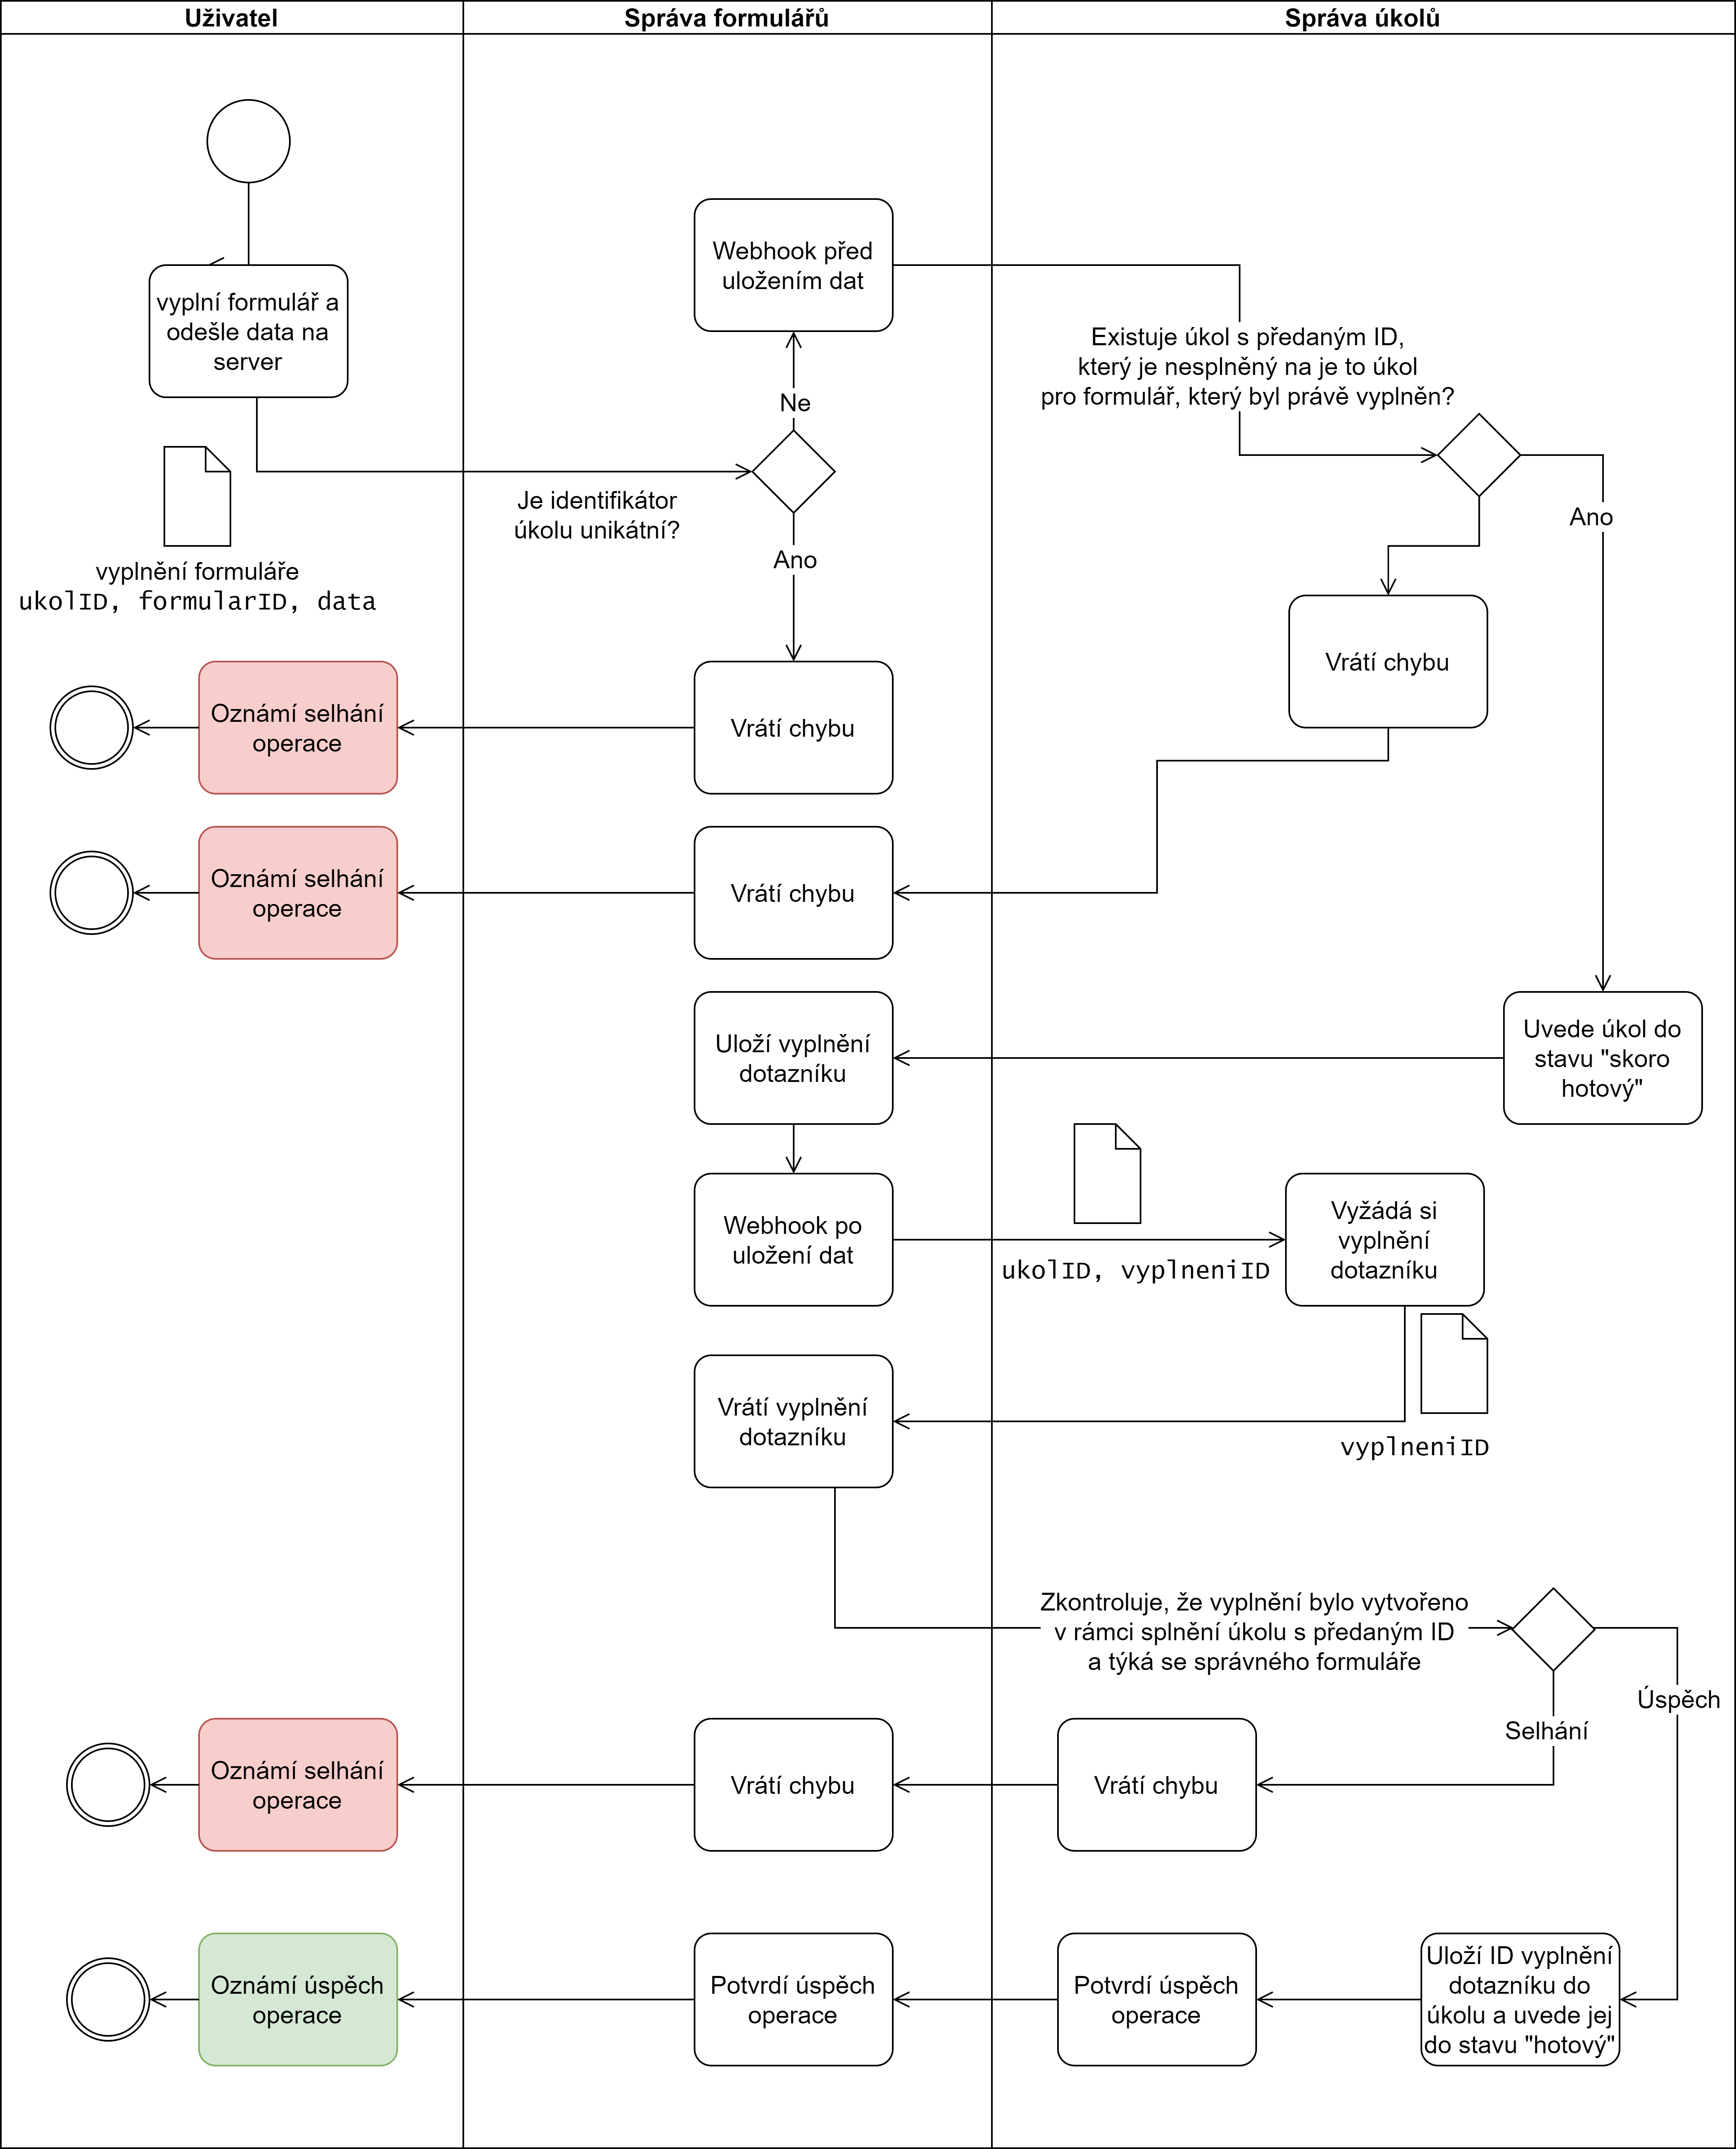
\includegraphics[width=\textwidth]{diagrams/activity.drawio}
    \caption{Diagram integrace systémů spravující úkoly a systému spravující formuláře}\label{fig:activity-diagram-task-and-form-integration}
\end{figure}

Požadavek na uložení vyplnění dotazníku spustí webhook.
V rámci reakce na tento webhook uvedeme úkol do stavu \texttt{skoro hotový}.
Tento stav slouží k tomu, aby nebylo možné vytvořit další vyplnění dotazníku v rámci stejného úkolu.
Tento mechanismus se nazývá \emph{semantic lock counter-measure}~\cite{semantic-lock-countermeasure-def}.
Stavy úkolu a přechody mezi nimi jsou popsány stavovým diagramem v jazyce UML na obr.~\ref{fig:task-state}.

Nyní popíšeme, jak je tento mechanismus využíván v našem systému.
Pokud požadavek na uložení vyplnění dotazníku spustí webhook, který proběhne před uložením do systému spravující formuláře, a následně selže operace uložení vyplnění dotazníku v systému spravující formuláře, tak úkol navždy zůstane ve stavu \texttt{skoro hotový}.
Pokud bychom se z tohoto stavu chtěli dostat, potřebovali bychom implementaci \href{https://microservices.io/patterns/data/saga.html}{ság}, která by zajistila provedení kompenzačních transakcí.
Popsaná situace je však natolik výjimečná, že se v tuto chvíli problematice věnovat nebudeme.
Vystačíme si s tím, že systém spravující formuláře nikdy nebude obsahovat vyplnění dotazníku, které vzniklo bez zadání úkolu.

\begin{figure}[H]
    \includegraphics[width=0.9\textwidth]{diagrams/taskState}
    \caption{Stavový diagram úkolů}\label{fig:task-state}
\end{figure}

Po uložení vyplnění dotazníku se zavolá druhý webhook, který zařídí uložení informace o identifikátoru vyplnění do úkolu.
Vzhledem k tomu, že se jedná o veřejně dostupný endpoint, tak je nutné ověřit poskytnutá data.
Musíme si tedy z úkolového systému vyžádat vyplnění dotazníku a zkontrolovat všechny náležitosti.
Pokud by se někdo pokusil spárovat úkol s formulářem, který je ve stavu \texttt{skoro hotový} na jiné vyplnění dotazníku než to, které způsobilo přechod úkolu do stavu \texttt{skoro hotový}, tak se mu to jistě nepovede.
Kdyby se někdo pokusil spárovat úkol s vyplněním dotazníku, který neodpovídá dotazníku zadaný úkolem, tak operace jistě selže.
V případě, že by se někdo pokusil spárovat jiné vyplnění stejného dotazníku, tak se mu to také nepovede.
Ono jiné vyplnění dotazníku by muselo mít jiný identifikátor úkolu v skrytém poli, protože systém spravující formuláře zajišťuje unikátnost těchto hodnot.
Jelikož víme, že již existuje vyplnění dotazníku, které má identifikátor úkolu v skrytém poli stejné jako identifikátor úkolu, který se právě snažíme napárovat, tak víme, že jakékoliv jiné vyplnění stejného dotazníku bude mít jiný identifikátor úkolu v skrytém poli.

\paragraph{Autentizace webhooků}

HTTP požadavky, které dělá systém spravující formuláře při tvorbě odevzdání formuláře na systém spravující úkoly, musí obsahovat autentizační hlavičky.
První možností je poskytnout systému spravující formuláře speciální přístupový token.
Toto však nelze provést pouze pro některé webhooky bez většího zásahu do zdrojového kódu systému spravující formuláře, ale pouze pro všechny webhooky najednou.
Navíc to situaci zbytečně komplikuje.

Druhá možnost je využití JWT tokenu z požadavku na vytvoření odevzdání formuláře, který je přijat systémem spravující formuláře.
Toto je dobrá možnost, ale open-source verze systému spravující formuláře tuto funkci nemá.
Nicméně není těžké ji do něj přidat.

Třetí možností je vyhnout se autentizaci webhooku pomocí přihlášení.
Místo toho bychom mohli vytvořit endpoint komponenty spravující úkoly, který je přístupný pouze z komponenty spravující formuláře.
Toto však znamená netriviální úpravy síťové infrastruktury.
Tyto úpravy jsou poměrně špatně udržovatelné.

Použijeme druhou možnost, jelikož má jednoduchou implementaci.
Provedené úpravy systému spravující formuláře jsou popsány v sekci~\ref{sec:konfigurace-a-modifikace-form.io}.


\chapter{Zhodnocení testování aplikace}\label{ch:zhodnoceni-testovani-aplikace}

Serverová část aplikace je testována pomocí unit testů.
Testujeme pouze veřejné rozhraní všech modulů.
Objekt fungující jako proxy databáze byl nahrazen mock objekty.
V testech kontrolujeme, zda-li se volají konkrétní metody na mock objektech s očekávanými parametry.
Toto je doporučený přístup object-relational mapping knihovny Prisma, který je popsán v \href{https://www.prisma.io/docs/guides/testing/unit-testing}{dokumentaci}.
Tento přístup se mi vůbec neosvědčil.
Kontrola volání konkrétních metod vytváří obrovskou závislost na vnitřní implementaci testovaných metod.
Testy jsou velmi těžko udržovatelné a navíc poměrně dlouhé a složité.
Kdybych začínal znovu, tak bych se snažil primárně testovat privátní metody, které obsahují veškerou logiku mimo databázové operace.
Přestože tento způsob je také silně závislý na vnitřní implementaci testovaného modulu, tak je udržitelnější a jednodušší na implementaci.
Pro testování metod obsahující databázové operace bych zvážil použití in-memory databáze\footnote{In-memory databáze je databáze spoléhající primárně na vnitřní paměť pro ukládání dat~\cite{in-memory-db-definition}}.

\chapter{Administrátorská příručka}\label{ch:administratorska-prirucka}

Tato kapitola popisuje, jak spravovat aplikaci z pohledu administrátora.
První jsou popsány kroky pro instalaci a konfiguraci aplikace v sekci~\ref{sec:instalace}.
Následně je popsáno spuštění aplikace v sekci~\ref{sec:spusteni-aplikace}.
V sekci~\ref{sec:tvorba-uzivatelskych-uctu} jsou popsány kroky pro tvorbu uživatelských účtů.
Nakonec jsou popsány přístupy k správcovským rozhraním jednotlivých částí aplikace v sekci~\ref{sec:sprava-aplikace}.


\section{Instalace a konfigurace}\label{sec:instalace}

Pro instalaci aplikace je potřeba mít nainstalovaný \href{https://www.docker.com/}{Docker} a \href{https://git-scm.com/}{Git}.

Celý projekt je zastřešen git repozitářem \href{https://github.com/PatrikTrefil/mental-health-monitoring-platform.git}{mental-health-monitoring-platform}.
Tento repozitář používá \href{https://git-scm.com/book/en/v2/Git-Tools-Submodules}{git submoduly}, jelikož zdrojový kód platformy Form.io je v jiném repozitáři.
Jedná se o repozitář \href{https://github.com/PatrikTrefil/mental-health-monitoring-platform-formio}{mental-health-monitoring-platform-formio}, což je fork repozitáře \href{https://github.com/formio/formio}{formio}, který obsahuje oficiální zdrojový kód platformy Form.io.
Pro instalaci aplikace je potřeba naklonovat repozitář \href{https://github.com/PatrikTrefil/mental-health-monitoring-platform.git}{mental-health-monitoring-platform} včetně submodulů, což lze provést následujícím příkazem:

\begin{verbatim}
git clone --recurse-submodules \
  https://github.com/PatrikTrefil/mental-health-monitoring-platform.git
\end{verbatim}

Klonování a inicializaci submodulů lze provést i pomocí následující sekvence příkazů:

\begin{verbatim}
git clone \
  https://github.com/PatrikTrefil/mental-health-monitoring-platform.git
cd mental-health-monitoring-platform
git submodule init # initialize configuration file
git submodule update # fetch submodule data
\end{verbatim}

Před spuštěním aplikace je potřeba dodat \texttt{.env} soubor do kořenu repozitáře pro konfiguraci prostředí.
Syntax konfiguračního souboru je popsána v \href{https://docs.docker.com/compose/environment-variables/env-file/}{dokumentaci Docker compose}.
Ukázkovou konfiguraci najdete v \texttt{.env.example}.
Zde je seznam proměnných prostředí, které je potřeba nastavit, a jejich význam:

\begin{description}
    \item[MONGO\_INITDB\_ROOT\_USERNAME] obsahuje uživatelské jméno pro přihlášení do MongoDB jako superuživatel (root).
    \item[MONGO\_INITDB\_ROOT\_PASSWORD] obsahuje heslo pro do MongoDB jako superuživatel (root).
    \item[FORMIO\_NODE\_CONFIG] obsahuje konfigurace Form.io aplikace.
    Hodnota by měla být ve formátu JSON\@.
    Výchozí hodnoty konfigurace jsou dostupné \href{https://github.com/formio/formio/blob/3.5.x/config/default.json}{zde}.
    Není potřeba nastavit všechny atributy konfiguračního objektu, ale pouze ty, které chceme přepsat.
    \item[FORMIO\_ROOT\_EMAIL] obsahuje e\babelhyphen{nobreak}mail pro přihlášení do Form.io aplikace jako superuživatel (root).
    \item[FORMIO\_ROOT\_PASSWORD] obsahuje heslo pro přihlášení do Form.io aplikace jako superuživatel (root).
    \item[FORMIO\_MONGO\_USER] obsahuje uživatelské jméno pro přístup Form.io apliakace do MongoDB\@.
    \item[FORMIO\_MONGO\_PASSWORD] obsahuje heslo pro přihlášení uživatele \texttt{FORMIO\_MONGO\_USER} do MongoDB\@.
    \item[DOMAIN\_NAME] obsahuje doménové jméno, na kterém bude aplikace dostupná (např.\ domena.cz, localhost).
    \item[NEXTAUTH\_SECRET] obsahuje klíč pro šifrování autentizačních tokenů.
\end{description}

Také je potřeba nainstalovat závislosti pro Form.io aplikaci:

\begin{verbatim}
cd src/formio && npm install
\end{verbatim}

Nyní aplikaci můžeme spustit pomocí návodu v sekci~\ref{sec:spusteni-aplikace}.
Poté je potřeba vytvořit první uživatelský účet, jak je popsáno v sekci~\ref{sec:tvorba-uzivatelskych-uctu}.


\section{Spuštění aplikace}\label{sec:spusteni-aplikace}

Předpokládáme, že aplikace byla nainstalována a konfigurována podle návodu v sekci~\ref{sec:instalace}.
Pro spuštění aplikace v produkčním módu spusťte následující příkaz z kořenového adresáře repozitáře:

\begin{verbatim}
docker compose up
\end{verbatim}

Po spuštění příkazu bude aplikace dostupná na \texttt{\href{http://localhost}{http://localhost}}.

Pokud se jedná o první spuštění aplikace, vytvořte prvního uživatele dle návodu v sekci~\ref{sec:tvorba-uzivatelskych-uctu}.

Pro spuštění aplikace ve vývojovém módu použijte následující příkaz:

\begin{verbatim}
docker compose --file ./docker-compose.yml \
  --file ./docker-compose.dev.yml \
  up
\end{verbatim}

Po spuštění příkazu bude aplikace dostupná na \texttt{\href{http://localhost:8080}{http://localhost:8080}}.
Na jednotlivé služby aplikace se lze připojit i přímo.
Mapování portů je definováno v \texttt{docker-compose.dev.yml}.


\section{Tvorba uživatelských účtů}\label{sec:tvorba-uzivatelskych-uctu}

Tato sekce popisuje kroky pro vytvoření uživatelských účtů.
Účty uživatelů libovolné role lze vytvořit pomocí webového rozhraní Form.io aplikace.
Po prvním spuštění aplikace je doporučeno vytvořit uživatele s rolí správce dotazníků.
Pro jednoduchost tvorby tohoto uživatele je připraven shell skript, jehož užití je popsáno v sekci~\ref{subsec:tvorba-uctu-pomoci-shell-skriptu}.

\subsection{Tvorba účtu pomocí webového rozhraní}\label{subsec:tvorba-uctu-pomoci-weboveho-rozhrani}

Účet lze vytvořit pomocí webového rozhraní Form.io aplikace, která je dostupná na \texttt{/formio/} po spuštění aplikace.
Po otevření rozhraní se zobrazí přihlašovací formulář.
Do formuláře vyplníme přihlašovací údaje adminisrátorského účtu, které jsme definovali v konfiguračním souboru při instalaci aplikace (viz sekce~\ref{sec:instalace}).
Po přihlášení je potřeba vyplnit formulář \textit{Správce dotazníků registrace}.
Uživatele \textit{nevytvářejte} skrze modul \textit{Resources}.

\subsection{Tvorba účtu pomocí shell skriptu}\label{subsec:tvorba-uctu-pomoci-shell-skriptu}

Pokud máte k dispozici příkaz \href{https://curl.se/}{\texttt{curl}}, tak uživatele \textit{s rolí správce dotazníků} můžete vytvořit pomocí shell skriptu \texttt{./create\_form\_manager.sh}.
Skript se spustí v interaktivním módu, pokud uživatel neposkytne všechny parametry programu.
Parametry programu lze take předat pomocí argumentů programu.
Parametry programu se odvíjí od konfigurace definované při instalaci aplikace (viz sekce~\ref{sec:instalace}).
Dokumentaci nástroje lze získat pomocí příkazu:

\begin{verbatim}
./create_form_manager.sh --help
\end{verbatim}


\section{Správa aplikace}\label{sec:sprava-aplikace}

Aplikace se skládá z několika částí, které je potřeba spravovat.
Zde je seznam částí aplikace a možné způsoby správy:

\begin{description}
    \item[Reverse proxy] Status stránka je dostupná na \texttt{/nginx\_status}.
    Když chceme zjistit zda-li reverse proxy běží, můžeme udělat HTTP GET požadavek na \texttt{/health}.
    Pokud je návratový kód 200, tak reverse proxy běží.
    \item[Monitoring] Monitoring služeb aplikace je dostupný na \texttt{/monitoring/}.
    Oficiální dokumentace k webovému rozhraní je dostupná online v anglickém jazyce \href{https://github.com/google/cadvisor/blob/master/docs/web.md}{zde}.
    Monitorovací aplikace poskytuje i API, které je dostupné na \texttt{/monitoring/api}.
    Oficiální dokumentace k API je dostupná online v anglickém jazyce \href{https://github.com/google/cadvisor/blob/master/docs/api.md}{zde}.
    \item[Form.io] Webové rozhraní a API aplikace Form.io je dostupné na \texttt{/formio/} po spuštění aplikace.
    Oficiální dokumentace k webovému rozhraní je dostupná online v anglickém jazyce \href{https://help.form.io/}{zde}.
    Oficiální dokumentace k API je dostupná online v anglickém jazyce \href{https://apidocs.form.io/}{zde}.
\end{description}


\chapter{Uživatelská dokumentace}\label{ch:uzivatelska-dokumentace}

V této kapitole popíšeme užívání aplikace z pohledu zaměstnance a plnitele.
Tyto role byly definovány v požadavku~\ref{itm:r-nr-1}.
První se podíváme na krok přihlášení, který je společný pro obě role, a následně na užívání aplikace.
Zaměstnanci a plnitelé přistupují na odlišné části aplikace, které jsou přístupné pouze pro jejich roli.
Z tohoto důvodu je popis uživání aplikace rozdělen do dvou sekcí dle role uživatele.


\section{Přihlášení}\label{sec:prihlaseni}

Proces přihlášení začíná na přihlašovací obrazovce (Obr.~\ref{fig:login-screenshot}), na kterou je uživatel přesměrován při vstupu do aplikace.
Před samotným přihlášením je nutno schválit používání cookies (Detaily jsou popsány v sekci~\ref{subsec:gdpr}).
Pro přihlášení uživatel zadá své přihlašovací údaje a stiskne tlačítko \uv{Přihlásit se}.
Následně je automaticky přesměrován na výchozí obrazovku pro svou roli.
Pokud zaměstnanec nemá účet, musí si požádat o vytvoření účtu u jiného zaměstnance s již existujícím účtem a dostatečným oprávněním, či u administrátora aplikace.
Pokud plnitel nemá účet, musí si požádat o vytvoření účtu u zaměstnance s již existujícím účtem a dostatečným oprávněním, či u administrátora aplikace.
Tvorba účtu zaměstnancem je popsána v sekci~\ref{subsec:sprava-uctu}.

\begin{figure}[H]
    \centering
    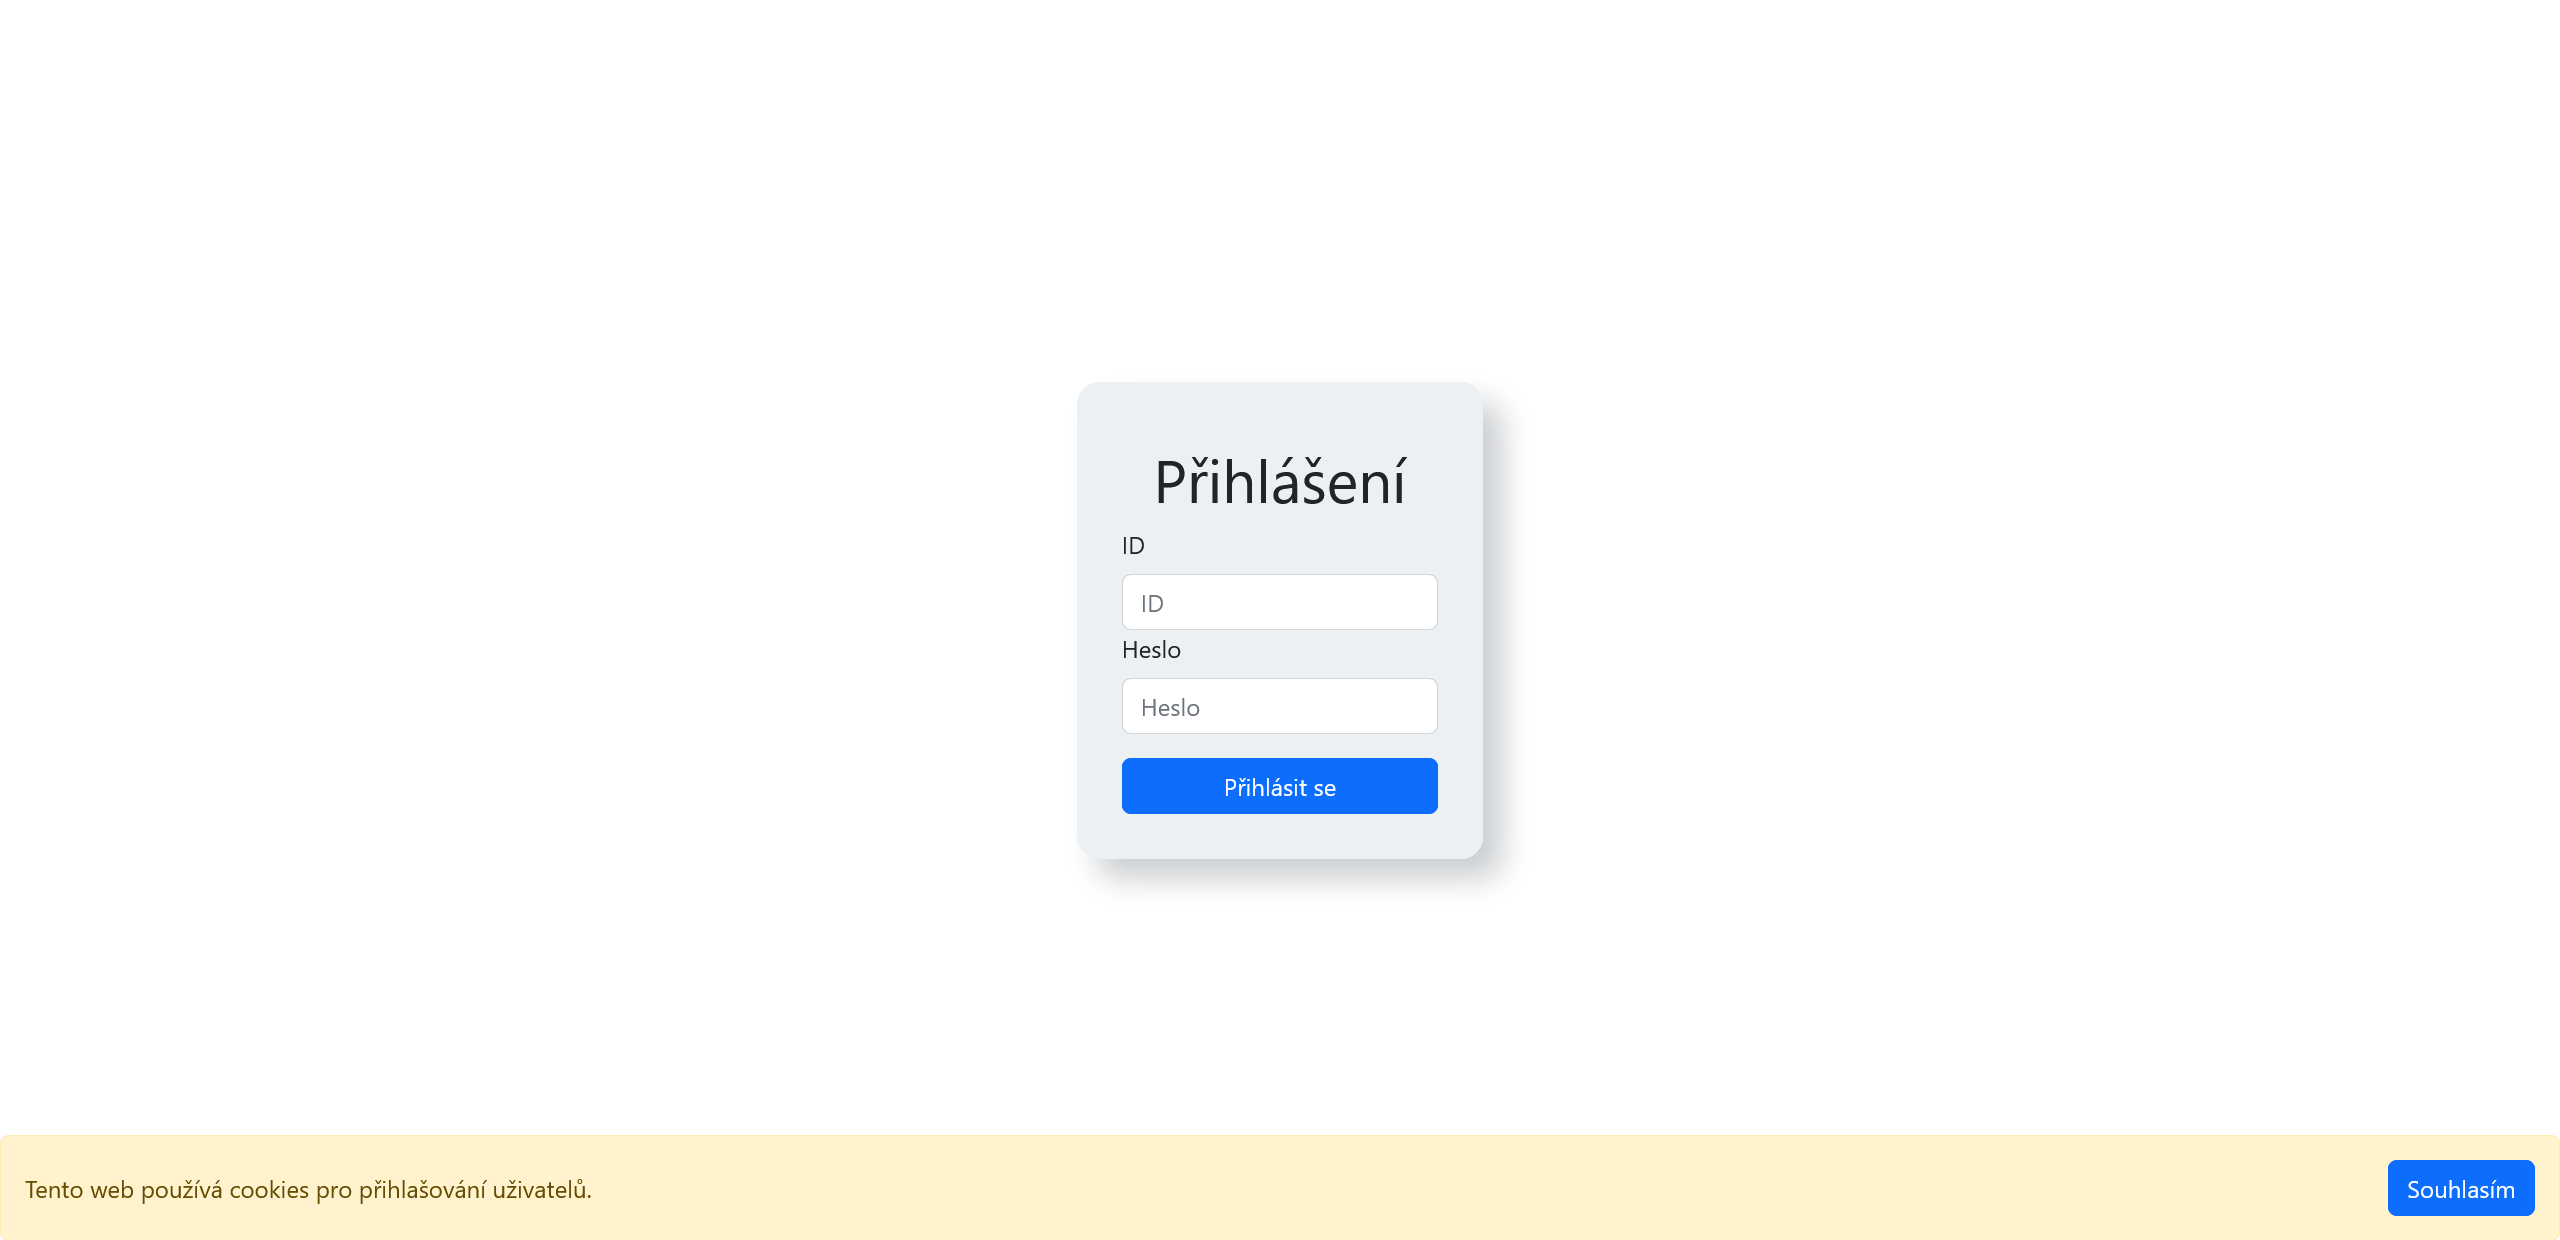
\includegraphics[width=\textwidth]{../img/screenshots/login}
    \caption{Přihlašovací obrazovka}\label{fig:login-screenshot}
\end{figure}


\section{Užívání aplikace z pohledu zaměstnance}\label{sec:uzivani-aplikace-z-pohledu-zamestnance}

Tato sekce popisuje užívání aplikace z pohledu zaměstnance.
Jsou zde popsány veškeré funkce, které byly identifikovány jako požadavky na funkcionalitu dostupnou zaměstnanci v kapitole~\ref{ch:analyza-pozadavku}.
Předpokládáme, že zaměstnanec má již vytvořený účet a přihlásil se do aplikace, jak je popsáno v sekci~\ref{sec:prihlaseni}, která se věnuje přihlášení a tvorbě účtu.
Po přihlášení je zaměstnanec automaticky přesměrován na výchozí obrazovku pro zaměstnance (Obr.~\ref{fig:sprava-formularu-screenshot}).

\subsection{Správa formulářů}\label{subsec:sprava-formularu}

Pro zadání úkolu plniteli je nutno nejprve vytvořit formulář.
Formuláře se vytváří v sekci \uv{Správa formulářů} (Obr.~\ref{fig:sprava-formularu-screenshot}).
Právo na tvorbu formulářů mají pouze zaměstnanci s rolí \uv{Správce dotazníků}.
Formuláře se vytváří pomocí tlačítka \uv{Nový formulář}.
Stisknutí tohoto tlačítka se dostaneme na stránku pro tvorbu formuláře (Obr.~\ref{fig:tvorba-formulare-screenshot}).
Pro vytvoření je potřeba zadat název formuláře do pole Název a přidat jednotlivé otázky taháním prvků z levého panelu do prostoru pro tvorbu formuláře.
Pole Identifikátor a Cesta se vyplní automaticky při zadání názvu a obvykle není třeba je měnit.
Jak vypočítat odvozené hodnoty v rámci vyhodnocení formuláře je popsáno v podsekci~\ref{subsubsec:vypocet-odvozenych-hodnot}.
Detailní dokumentace k tvorbě formulářů je dostupná online v anglickém jazyce na \href{https://help.form.io/userguide/form-building}{tomto odkazu}.
Formulář uložíme do systému pomocí tlačítka \uv{Vytvořit formulář}.
Obrazovka pro správu formulářů (Obr.~\ref{fig:sprava-formularu-screenshot}) nám nabízí několik dalších funkcí.
Již existující formuláře můžeme upravovat pomocí tlačítka \uv{Upravit} nebo mazat pomocí tlačítka \uv{Smazat}.
Úpravy formulářů mohou ovlivnit již existující odevzdání formulářů a proto se doporučuje tuto funkci používat pouze pro drobné opravy.

\begin{figure}[H]
    \centering
    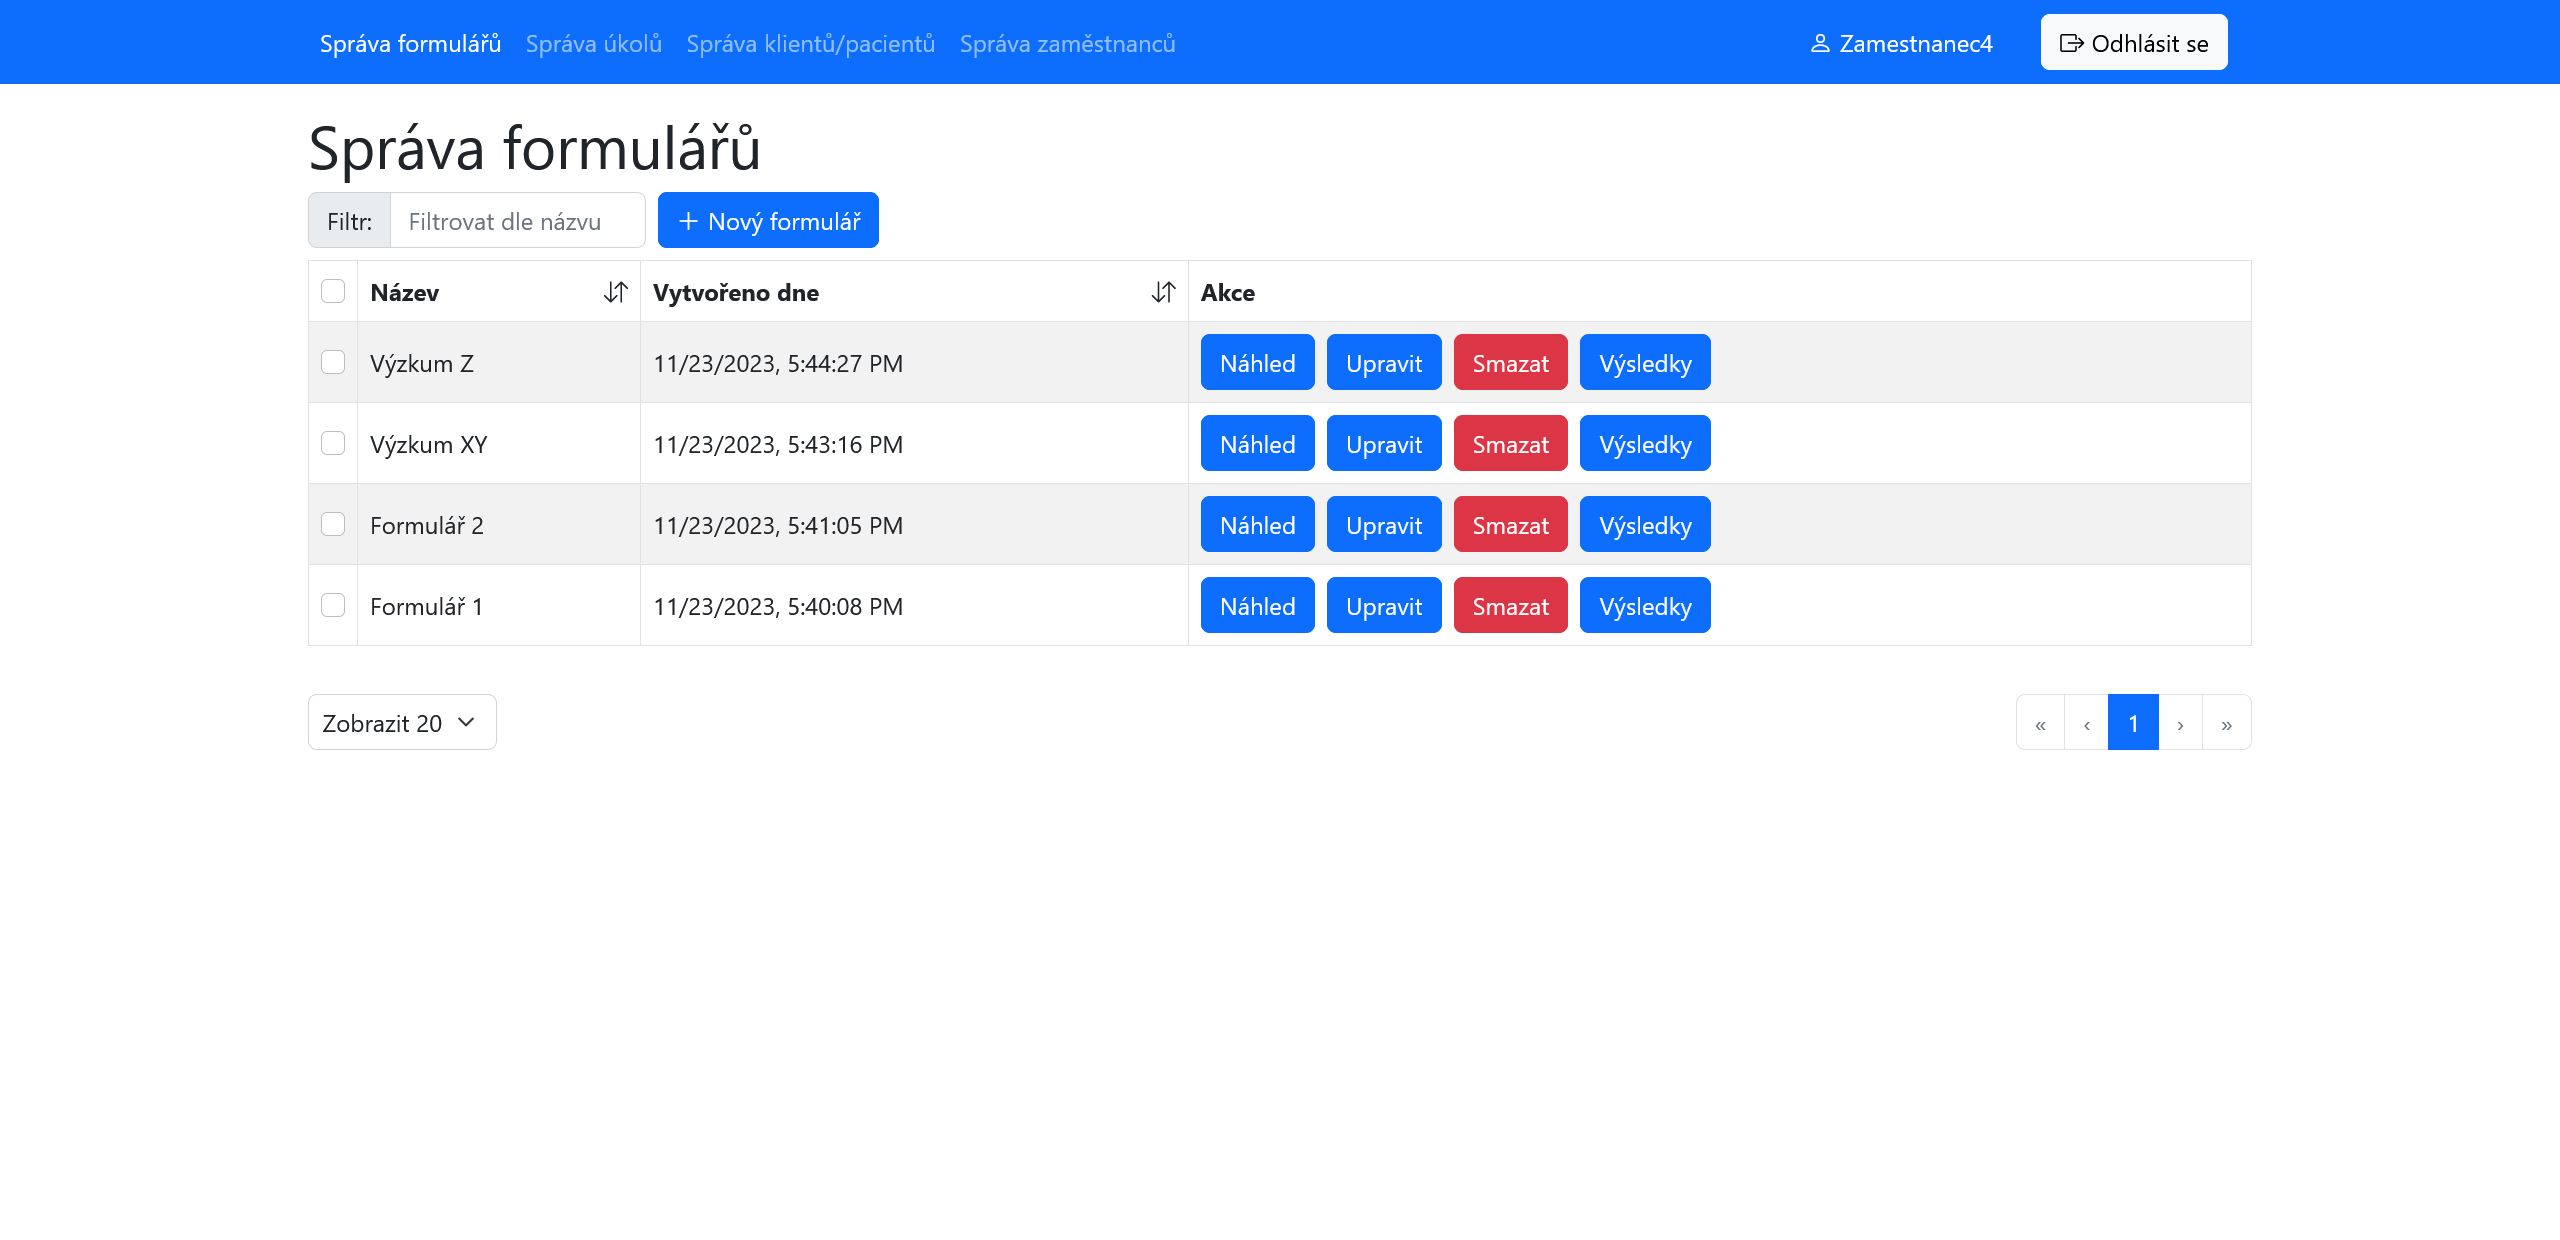
\includegraphics[width=\textwidth]{../img/screenshots/sprava-formularu}
    \caption{Správa formulářů aplikace}\label{fig:sprava-formularu-screenshot}
\end{figure}

\begin{figure}[H]
    \centering
    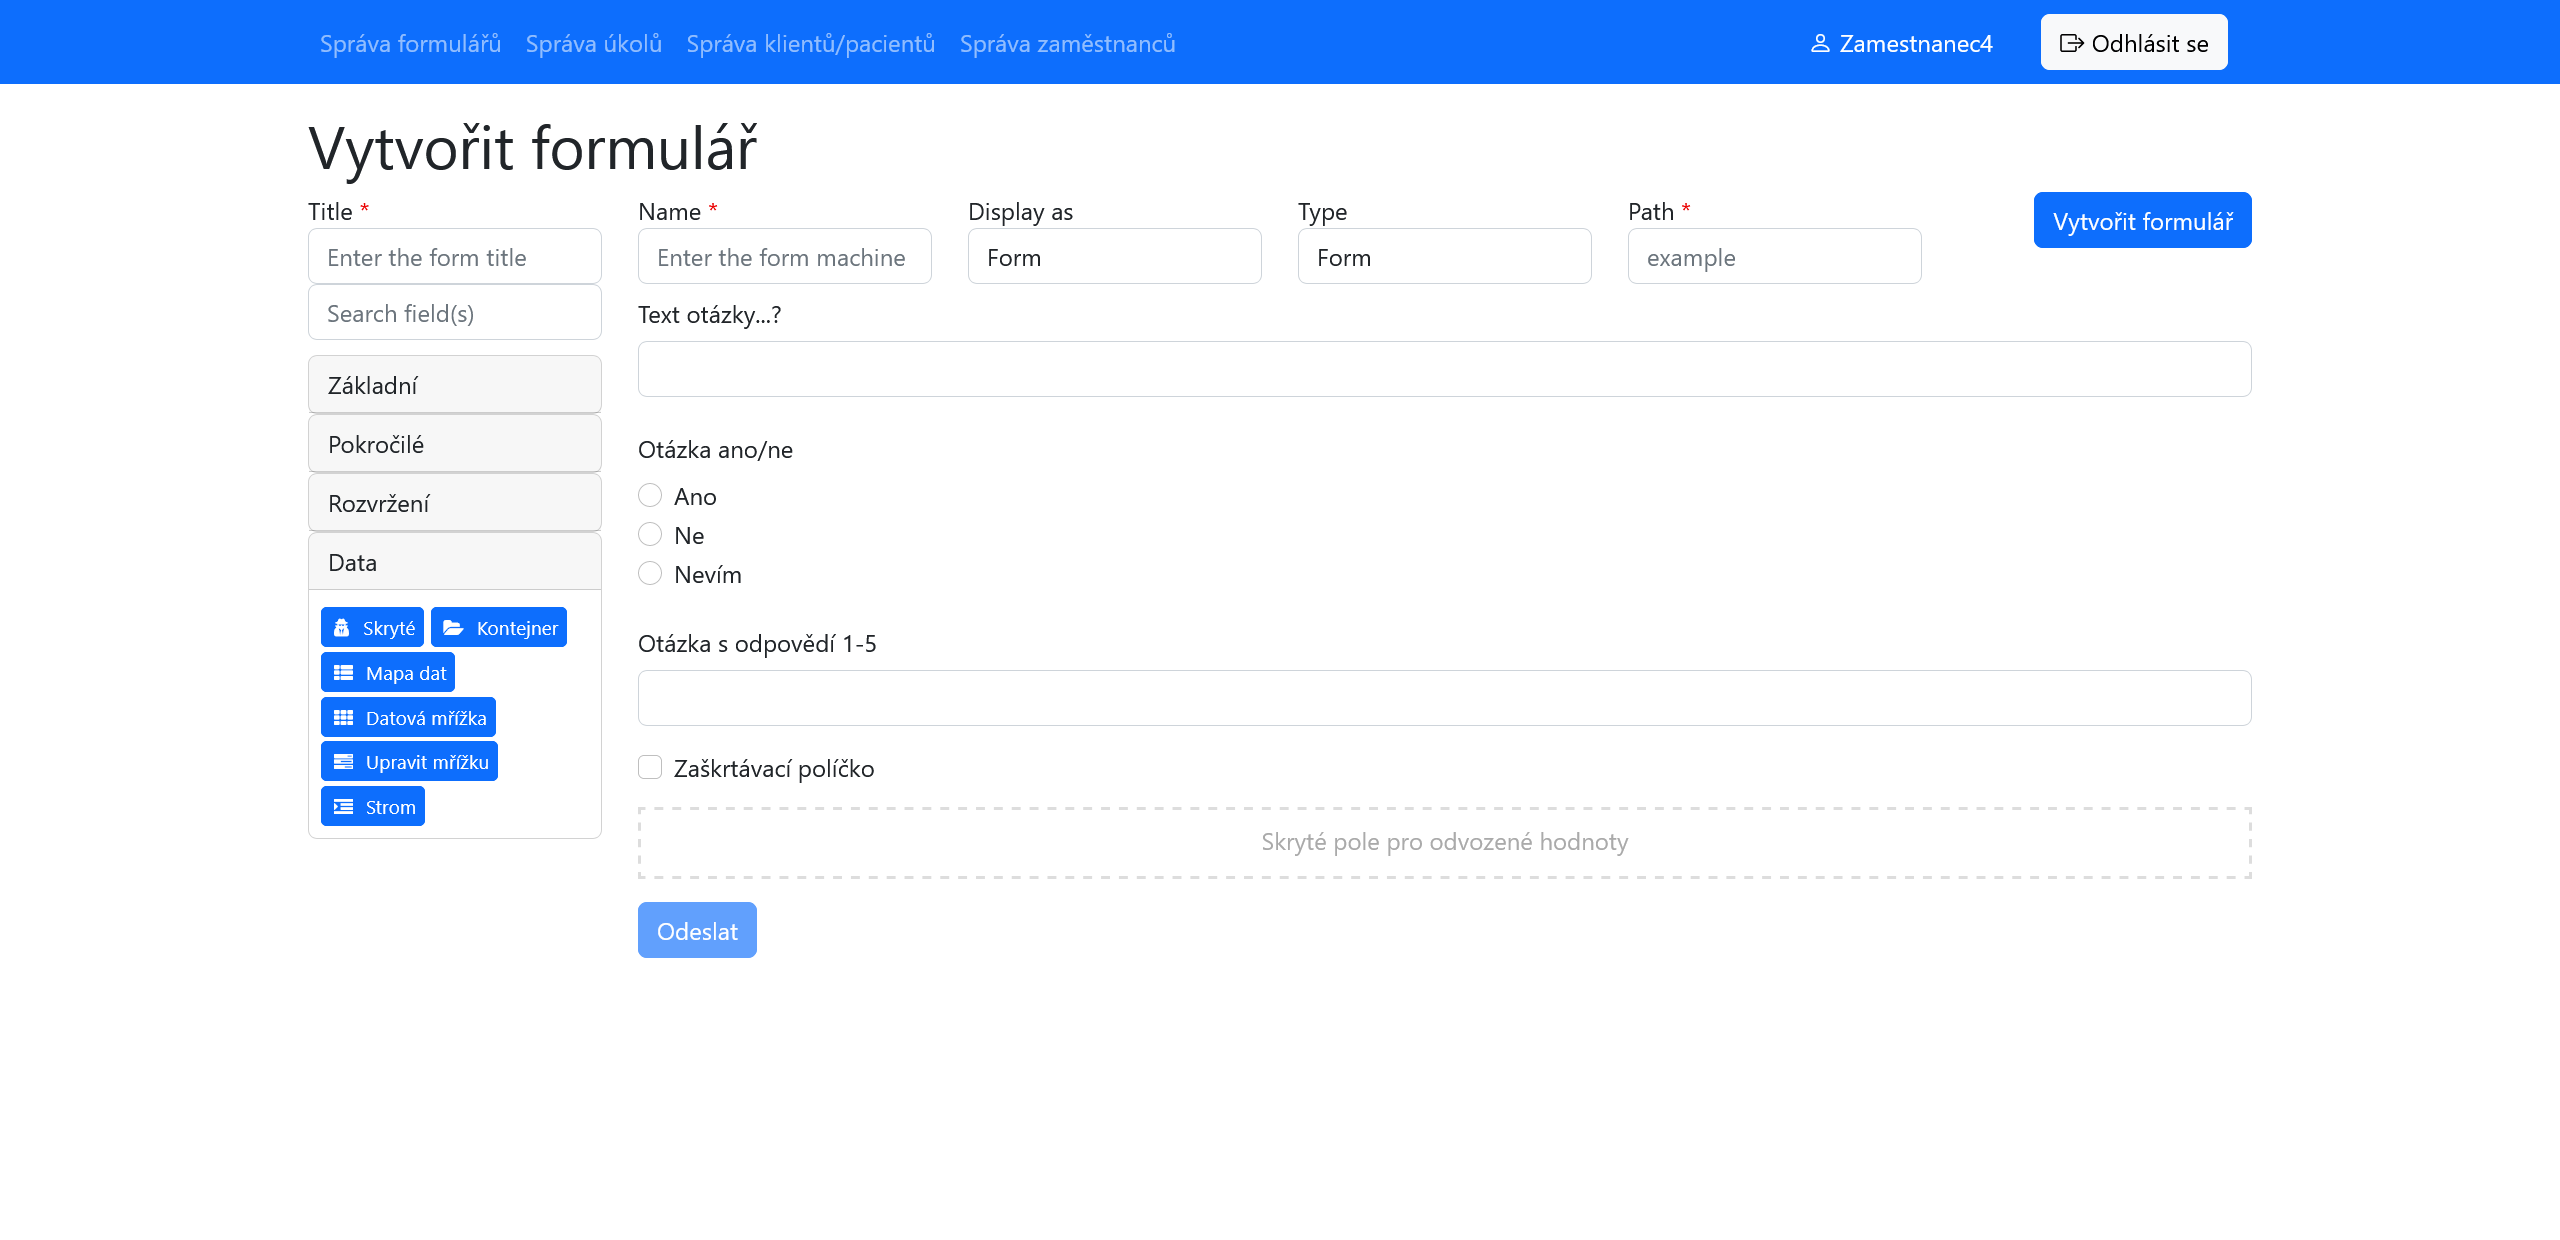
\includegraphics[width=\textwidth]{../img/screenshots/tvorba-formulare}
    \caption{Správa formulářů aplikace}\label{fig:tvorba-formulare-screenshot}
\end{figure}

\subsubsection{Výpočet odvozených hodnot}\label{subsubsec:vypocet-odvozenych-hodnot}

Pokud chceme formulář automaticky vyhodnotit na základě odpovědí plnitele, použijeme prvek \uv{Skryté} z kategorie \uv{Data} z levého panelu.
Po přidání prvku se zobrazí jeho nastavení (Obr.~\ref{fig:odvozena-hodnota-nastaveni}).
Vzorec pro výpočet hodnoty můžeme zadat do sekce \uv{Vypočtená hodnota} v kartě \uv{Data} (Obr.~\ref{fig:odvozena-hodnota-vzorec-a-server}).
Vzorec se zapisuje v programovacím jazyce \href{https://developer.mozilla.org/en-US/docs/Web/JavaScript}{JavaScript}.
Všechny hodnoty odpovědí jsou dostupné na objektu \texttt{data}.
Vzorec používá názvy vlastností jako klíče na tomto objektu.
Pro použití konkrétní můžeme použít tečkovou notaci \texttt{data.nazevVlastnosti} nebo notaci s hranatými závorkami \texttt{data["nazevVlastnosti"]}.
Název vlastnosti lze pro každý prvek nastavit v menu nastavení v poli \uv{Název vlastnosti} v kartě \uv{API} (Obr.~\ref{fig:odvozena-hodnota-nastaveni-nazev}).
Výsledek vzorce uložíme do proměnné \texttt{value}.
Např.\ pro součet hodnoty odpovědí s názvy \uv{a} a \uv{b} bychom použili vzorec \texttt{value = data.a + data.b}.
Pokud je nevhodné, aby uživatel viděl způsob výpočtu odvozené hodnoty nebo mohl získat vypočtenou hodnotu, tak je nutné v nastavení prvku zvolit možnost \uv{Vypočítat hodnotu na serveru} (Obr.~\ref{fig:odvozena-hodnota-vzorec-a-server}).
Nastavení prvku uložíme stisknutím tlačítka \uv{Uložit}.
Kdybychom chtěli nastavení prvku znovu upravit, tak se na obrazovku nastavení dostaneme stisknutím tlačítka s ozubeným kolečkem v pravém horním rohu prvku (Obr.~\ref{fig:odvozena-hodnota-ozubene-kolo}).

\begin{figure}[H]
    \centering
    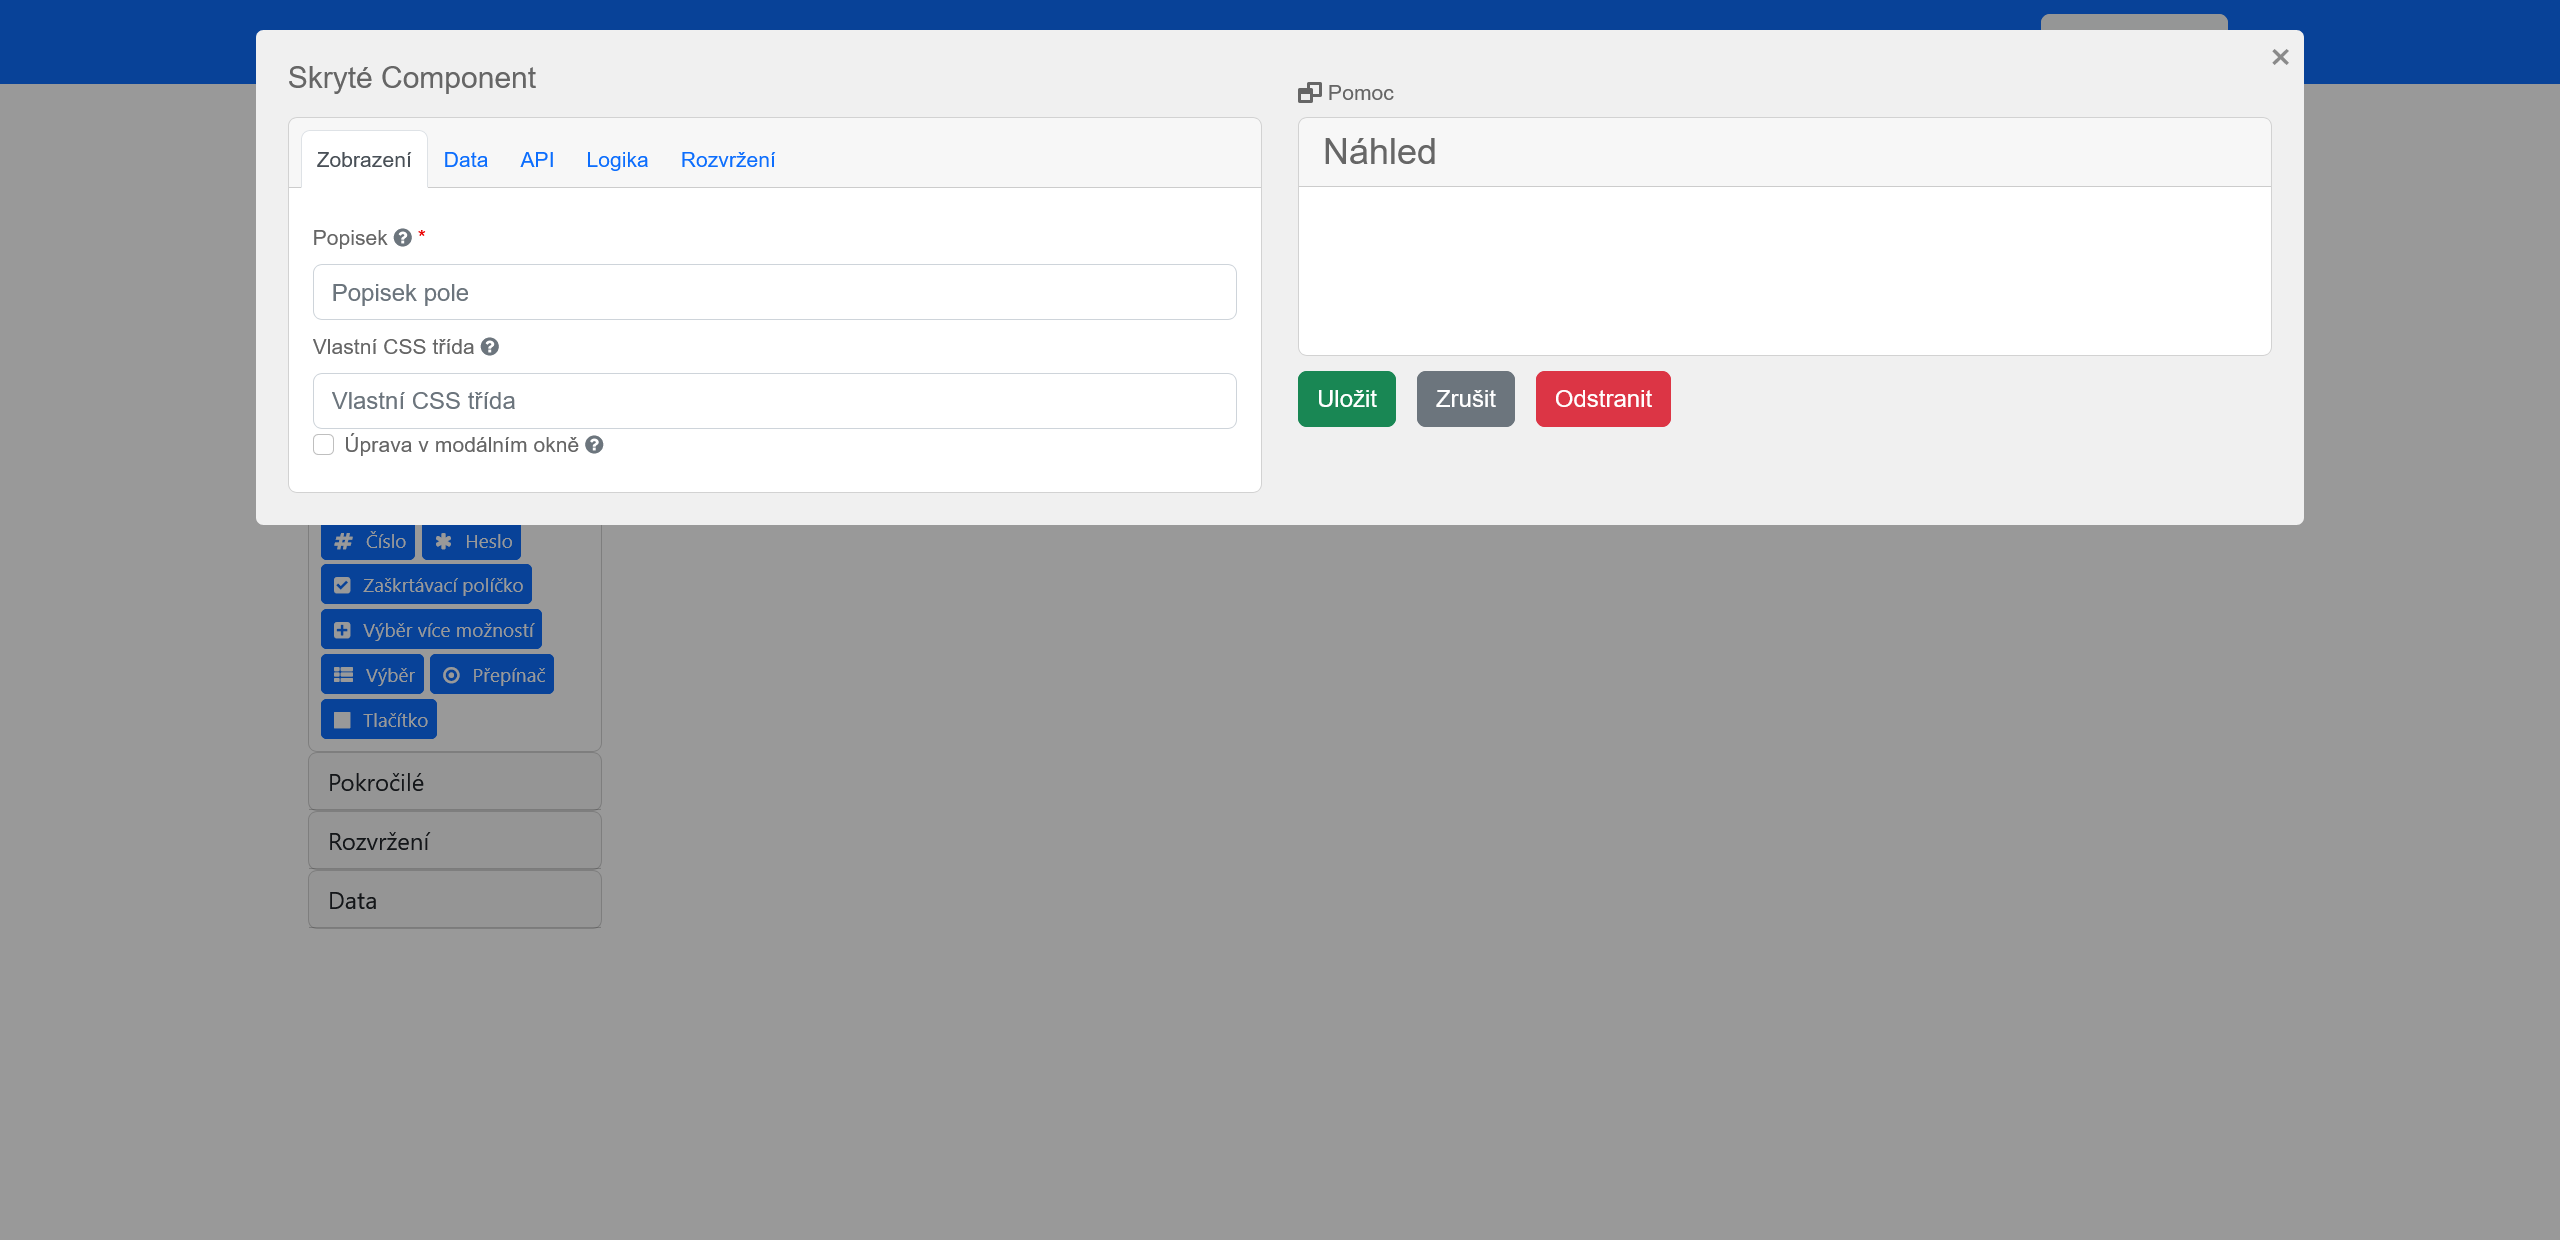
\includegraphics[width=\textwidth]{../img/screenshots/odvozena-hodnota-nastaveni}
    \caption{Karta Zobrazení v nastavení prvku Skryté}\label{fig:odvozena-hodnota-nastaveni}
\end{figure}

\begin{figure}[H]
    \centering
    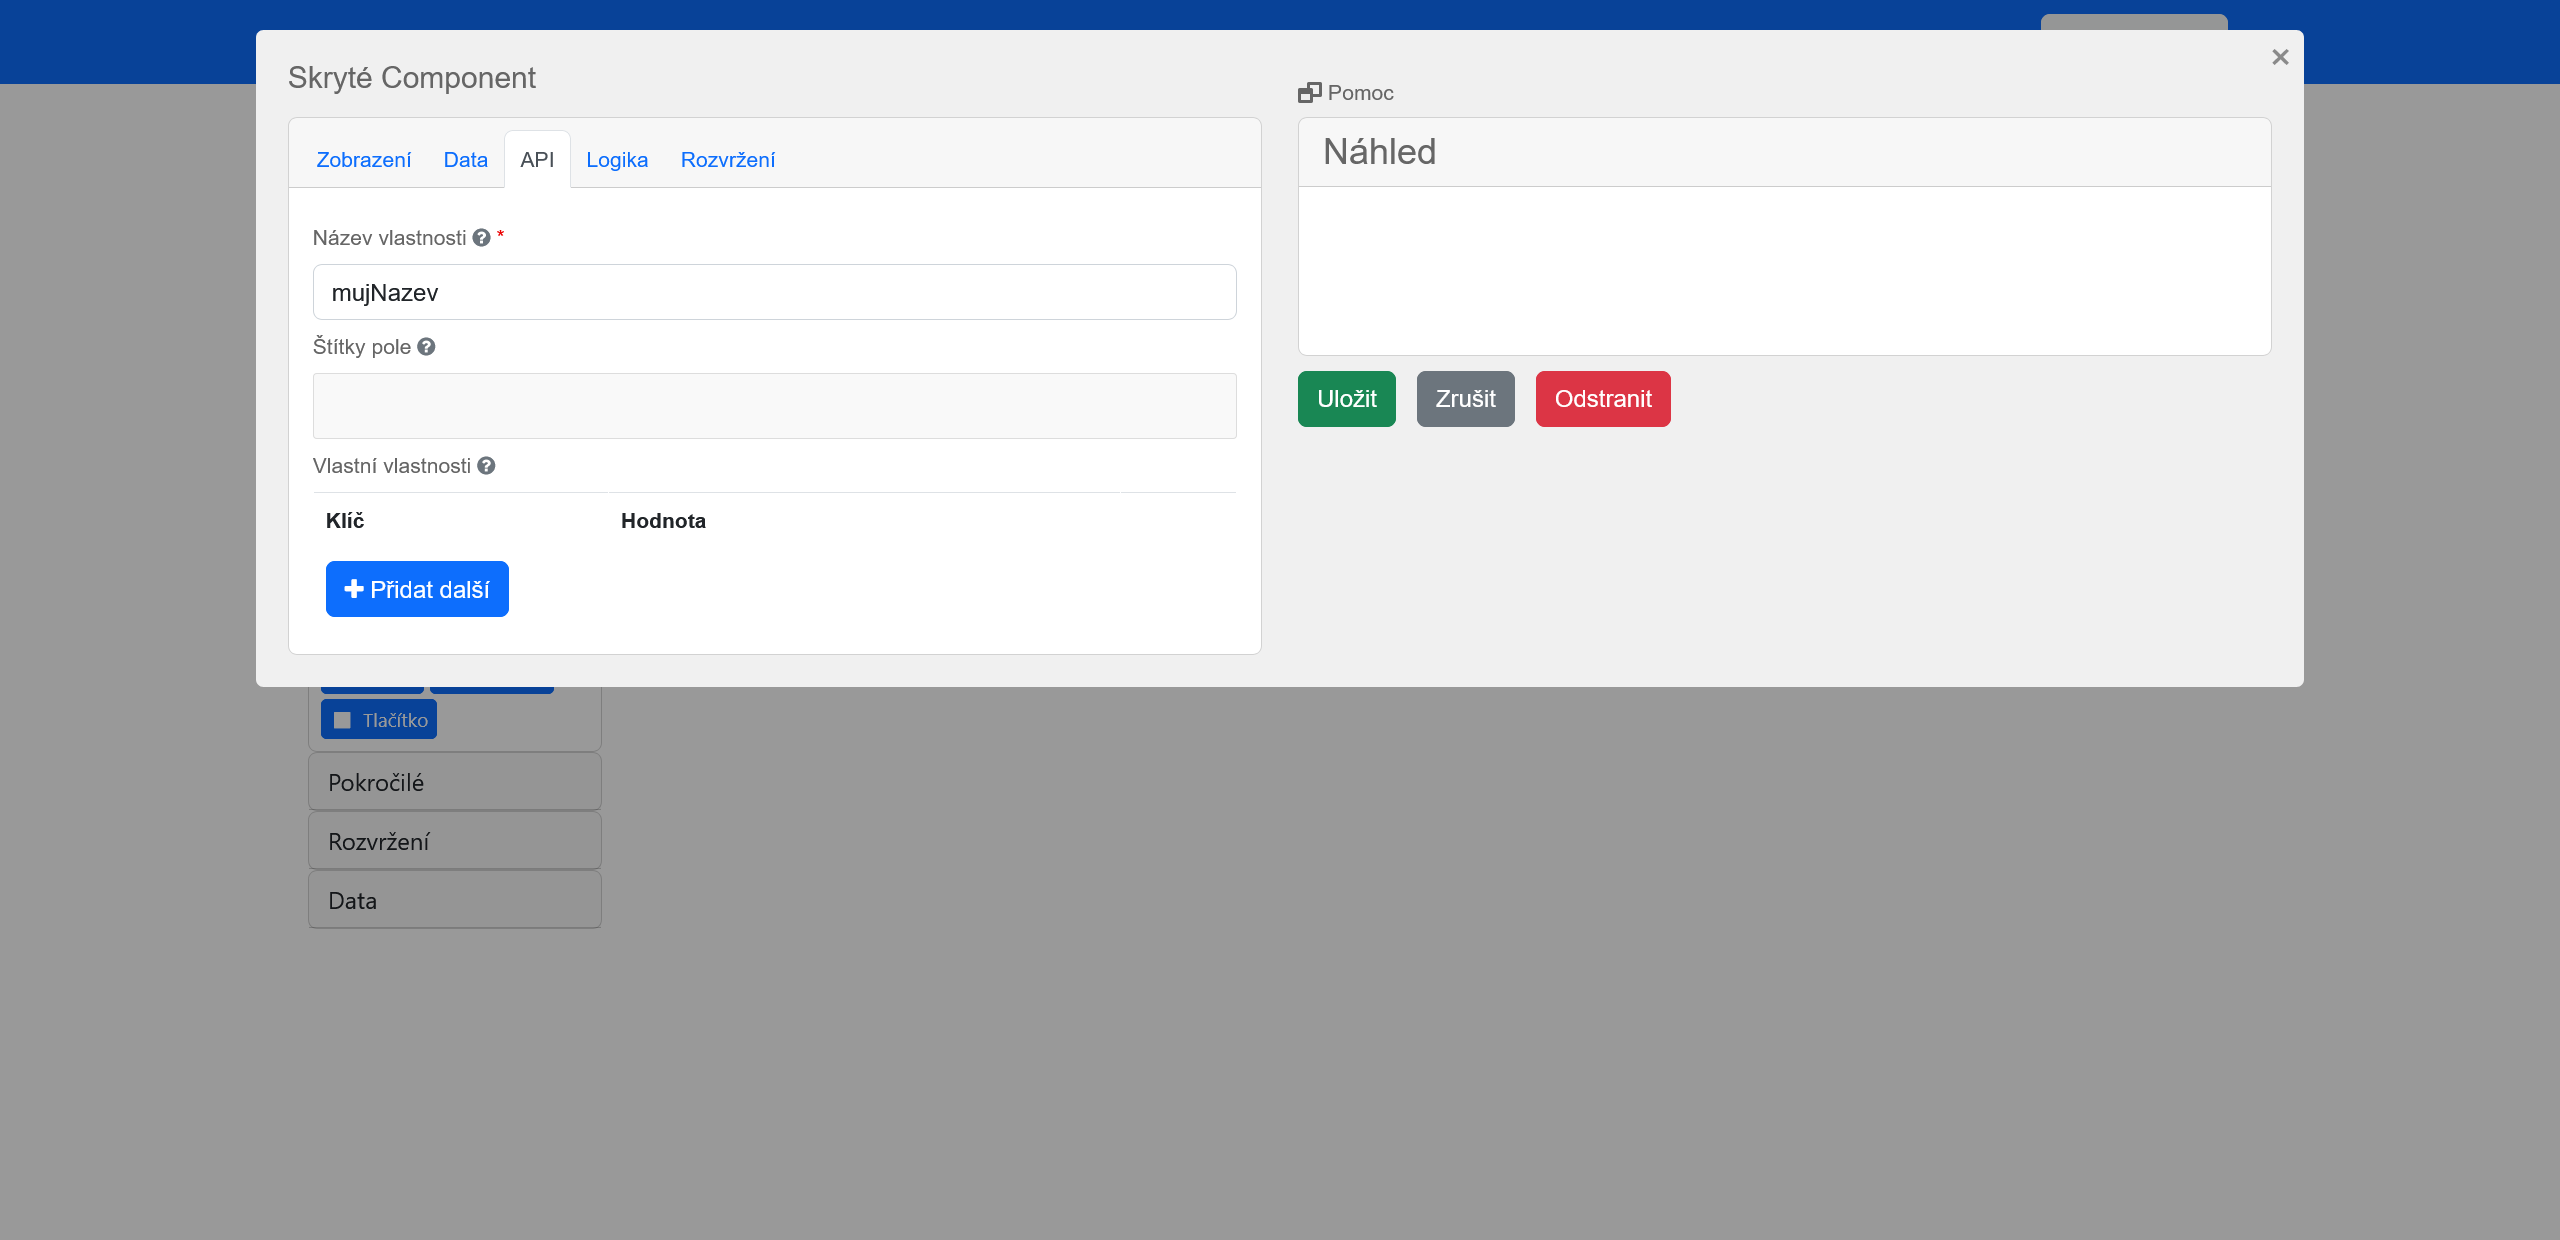
\includegraphics[width=\textwidth]{../img/screenshots/odvozena-hodnota-nastaveni-nazvu}
    \caption{Karta API v nastavení prvku Skryté}\label{fig:odvozena-hodnota-nastaveni-nazev}
\end{figure}

\begin{figure}[H]
    \centering
    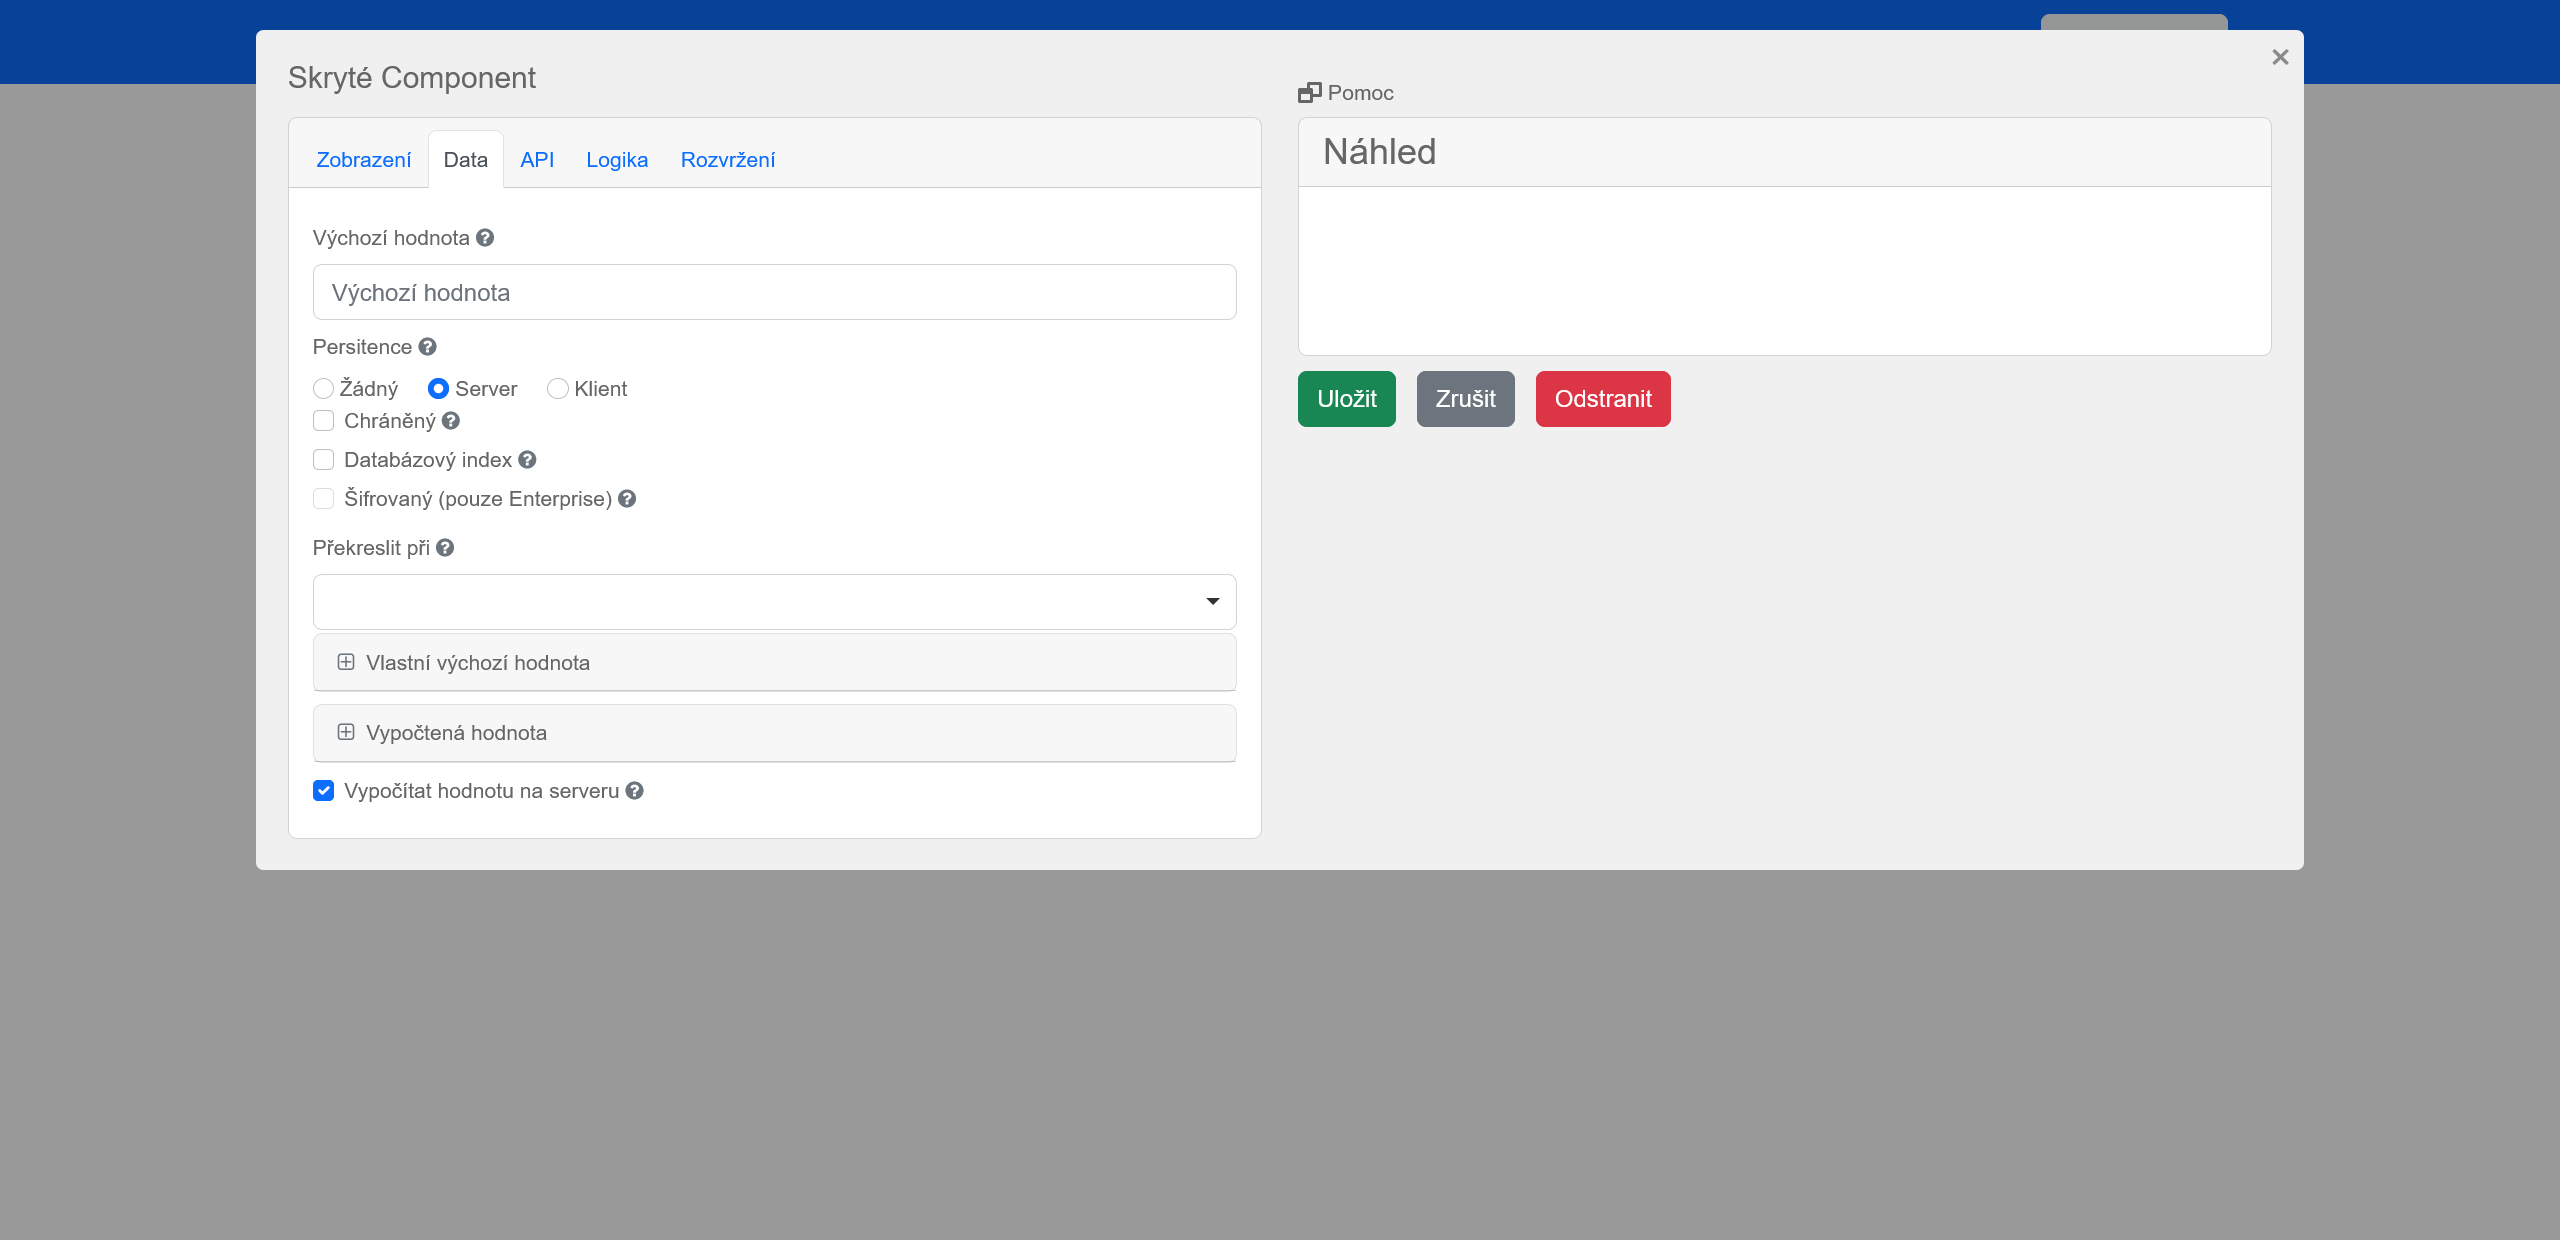
\includegraphics[width=\textwidth]{../img/screenshots/odvozena-hodnota-vzorec-a-server}
    \caption{Karta Data v nastavení prvku Skryté}\label{fig:odvozena-hodnota-vzorec-a-server}
\end{figure}

\begin{figure}[H]
    \centering
    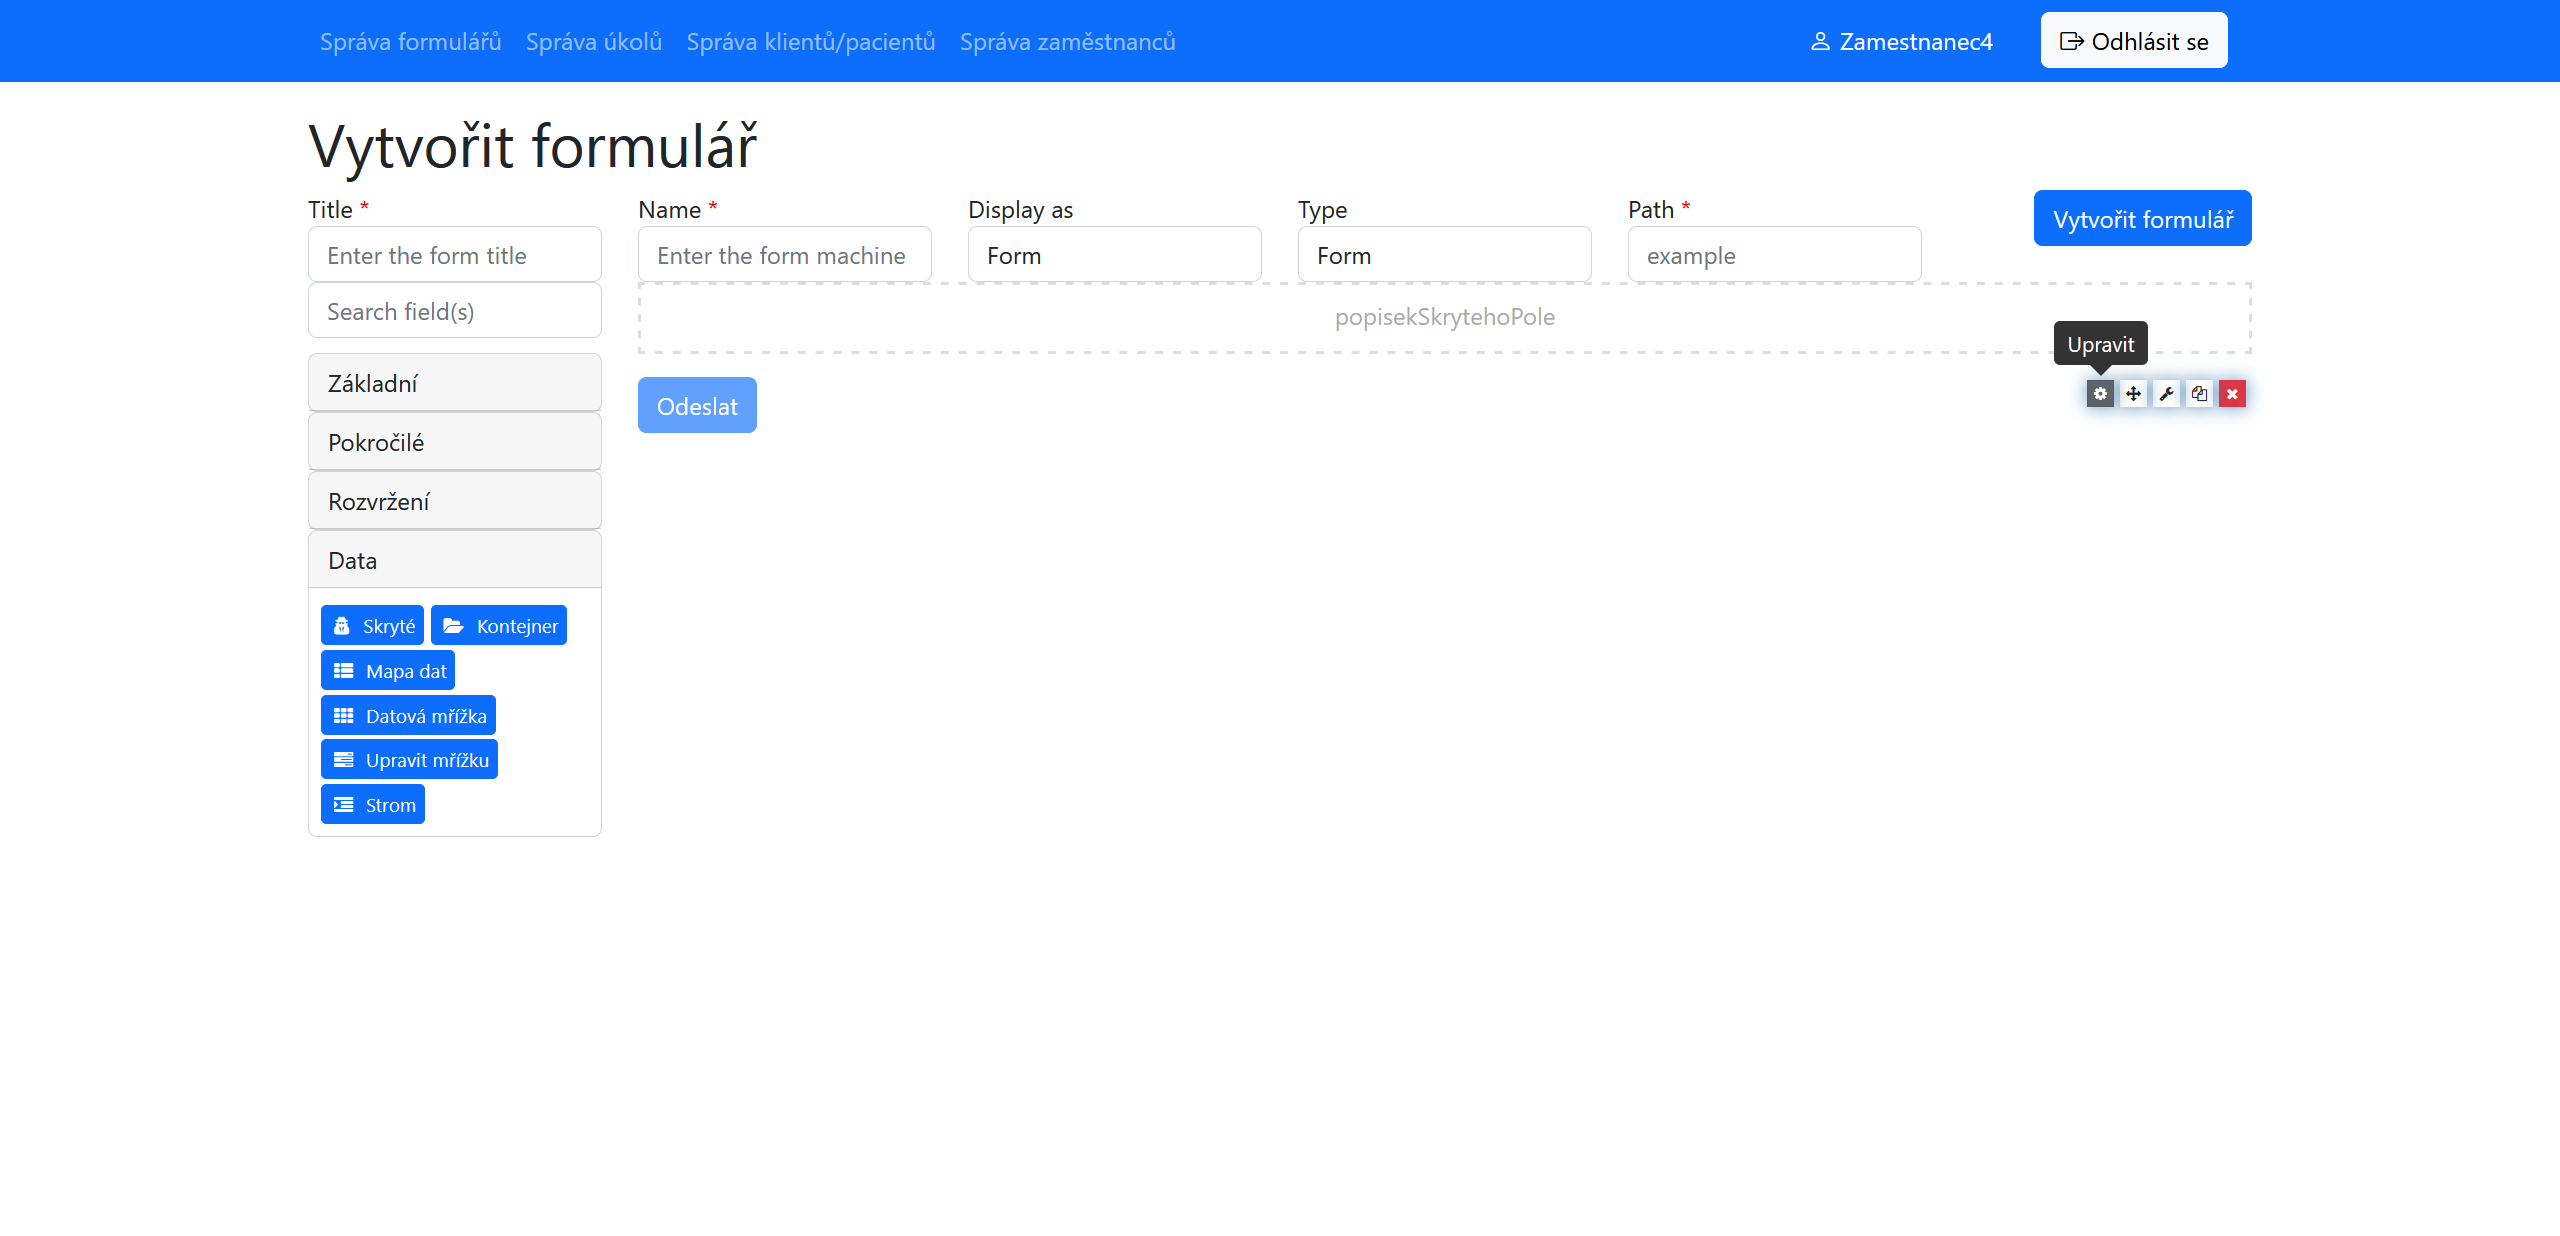
\includegraphics[width=\textwidth]{../img/screenshots/odvozena-hodnota-ozubene-kolo}
    \caption{Zobrazení menu nastavení prvku}\label{fig:odvozena-hodnota-ozubene-kolo}
\end{figure}

\subsection{Správa plnitelů}\label{subsec:sprava-plnitelu}

Pro zadání úkolu plniteli je nutno nejprve vytvořit uživatelský účet pro plnitele.
Účty plnitelů se vytváří v sekci \uv{Správa plnitelů} (Obr.~\ref{fig:sprava-plnitelu-screenshot}).
Nový účet vytvoříme pomocí tlačítka \uv{Založit účet nového klienta/pacienta}.
Pro vytvoření účtu je potřeba zadat identifikátor plnitele, který je unikátní v rámci celé aplikace, a heslo.
Plnitel si může heslo změnit po přihlášení do aplikace.

\begin{figure}[H]
    \centering
    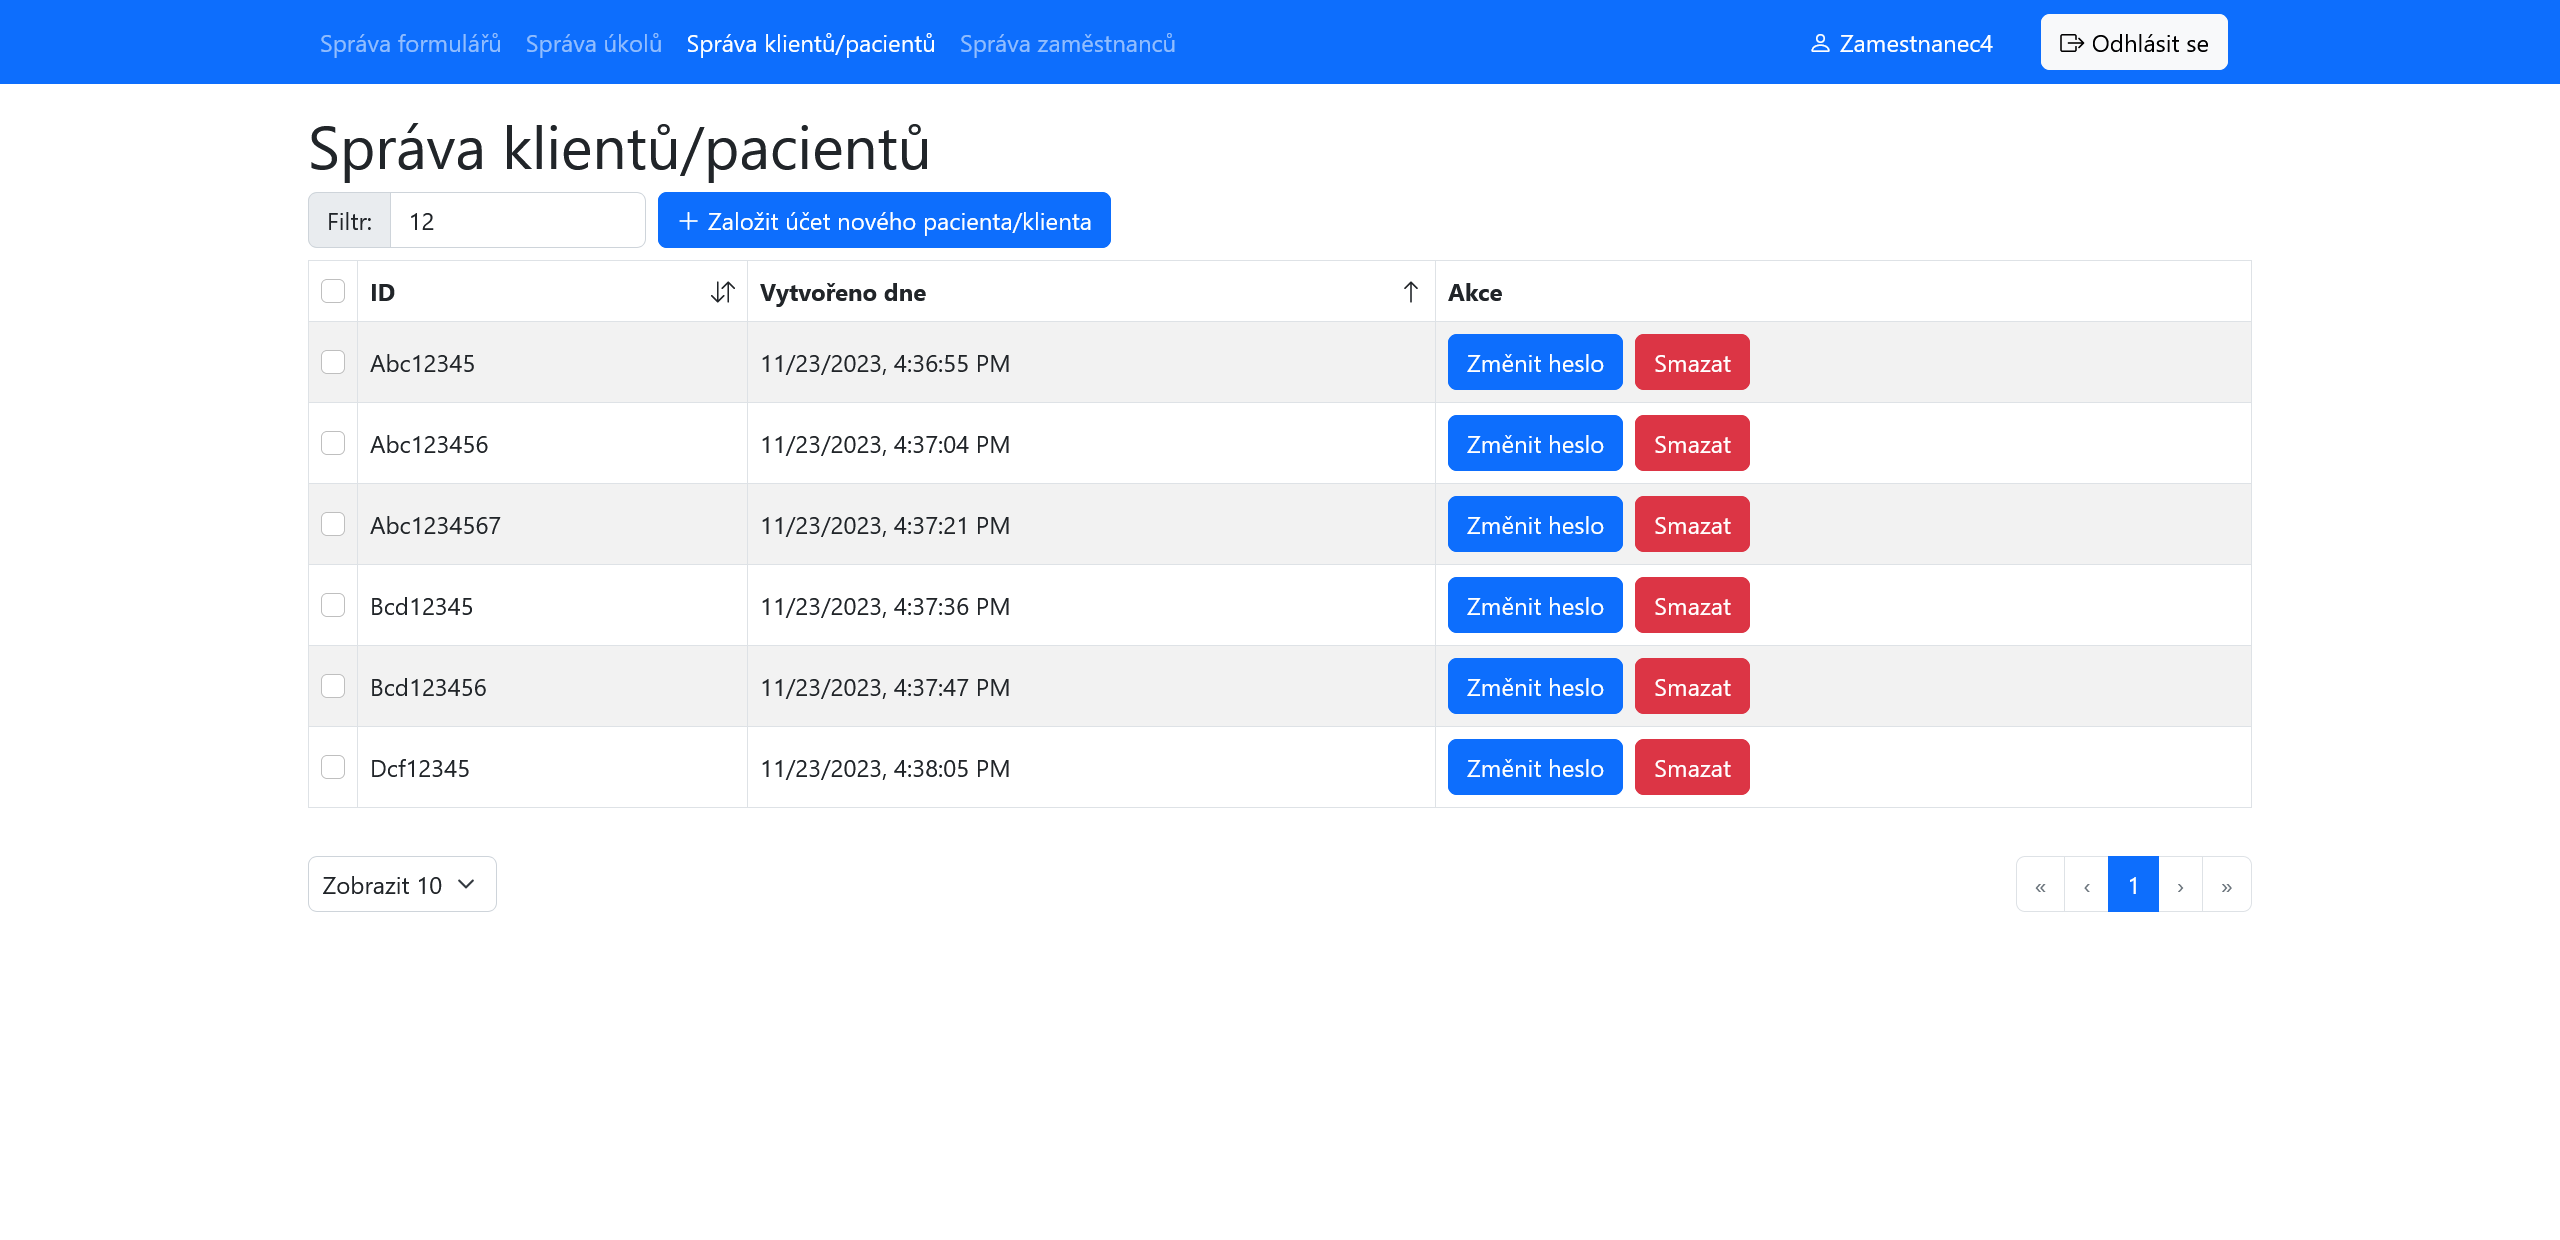
\includegraphics[width=\textwidth]{../img/screenshots/sprava-plnitelu}
    \caption{Správa účtů plnitelů}\label{fig:sprava-plnitelu-screenshot}
\end{figure}

\subsection{Správa úkolů}\label{subsec:sprava-ukolu}

Nyní můžeme vytvořit úkol pro plnitele.
Úkoly se vytváří v sekci \uv{Správa úkolů} (Obr.~\ref{fig:sprava-ukolu-screenshot}).
Nový úkol vytvoříme pomocí tlačítka \uv{Nový úkol}.
Stisknutím tohoto tlačítka se dostaneme na stránku pro tvorbu úkolu (Obr.~\ref{fig:tvorba-ukolu-screenshot}).
Pro vytvoření je potřeba zadat název úkolu, vybrat formulář, který má plnitel vyplnit, a vybrat plnitele.
Při tvorbě je možno zvolit více plnitelů a tím zadat více úkolů najednou.
K úkolu můžeme volitelně přidat popis, start, deadline a opakování.
Start úkolu je datum a čas, od kdy je možné úkol splnit.
Deadline úkolu je datum a čas, do kdy je možné úkol splnit.
Start a deadline byly takto definovány v kapitole~\ref{ch:analyza-pozadavku}.
Můžeme povolit překročení deadline, ale standardně je po deadline úkol uzavřen a nelze jej splnit.
Obrazovka pro konfiguraci deadline je zobrazena na obrázku~\ref{fig:tvorba-ukolu-deadline-screenshot}.
Při nastavení opakování je vytvořeno více úkolu najednou pro jednoho uživatele.
Pokud chceme vytvořit opakující se úkol, tak je nutné také definovat deadline, který je vždy posunut o interval specifikovaný v nastavení opakování.
Obrazovka pro konfiguraci opakování je zobrazena na obrázku~\ref{fig:tvorba-ukolu-opakovani-screenshot}.

\begin{figure}[H]
    \centering
    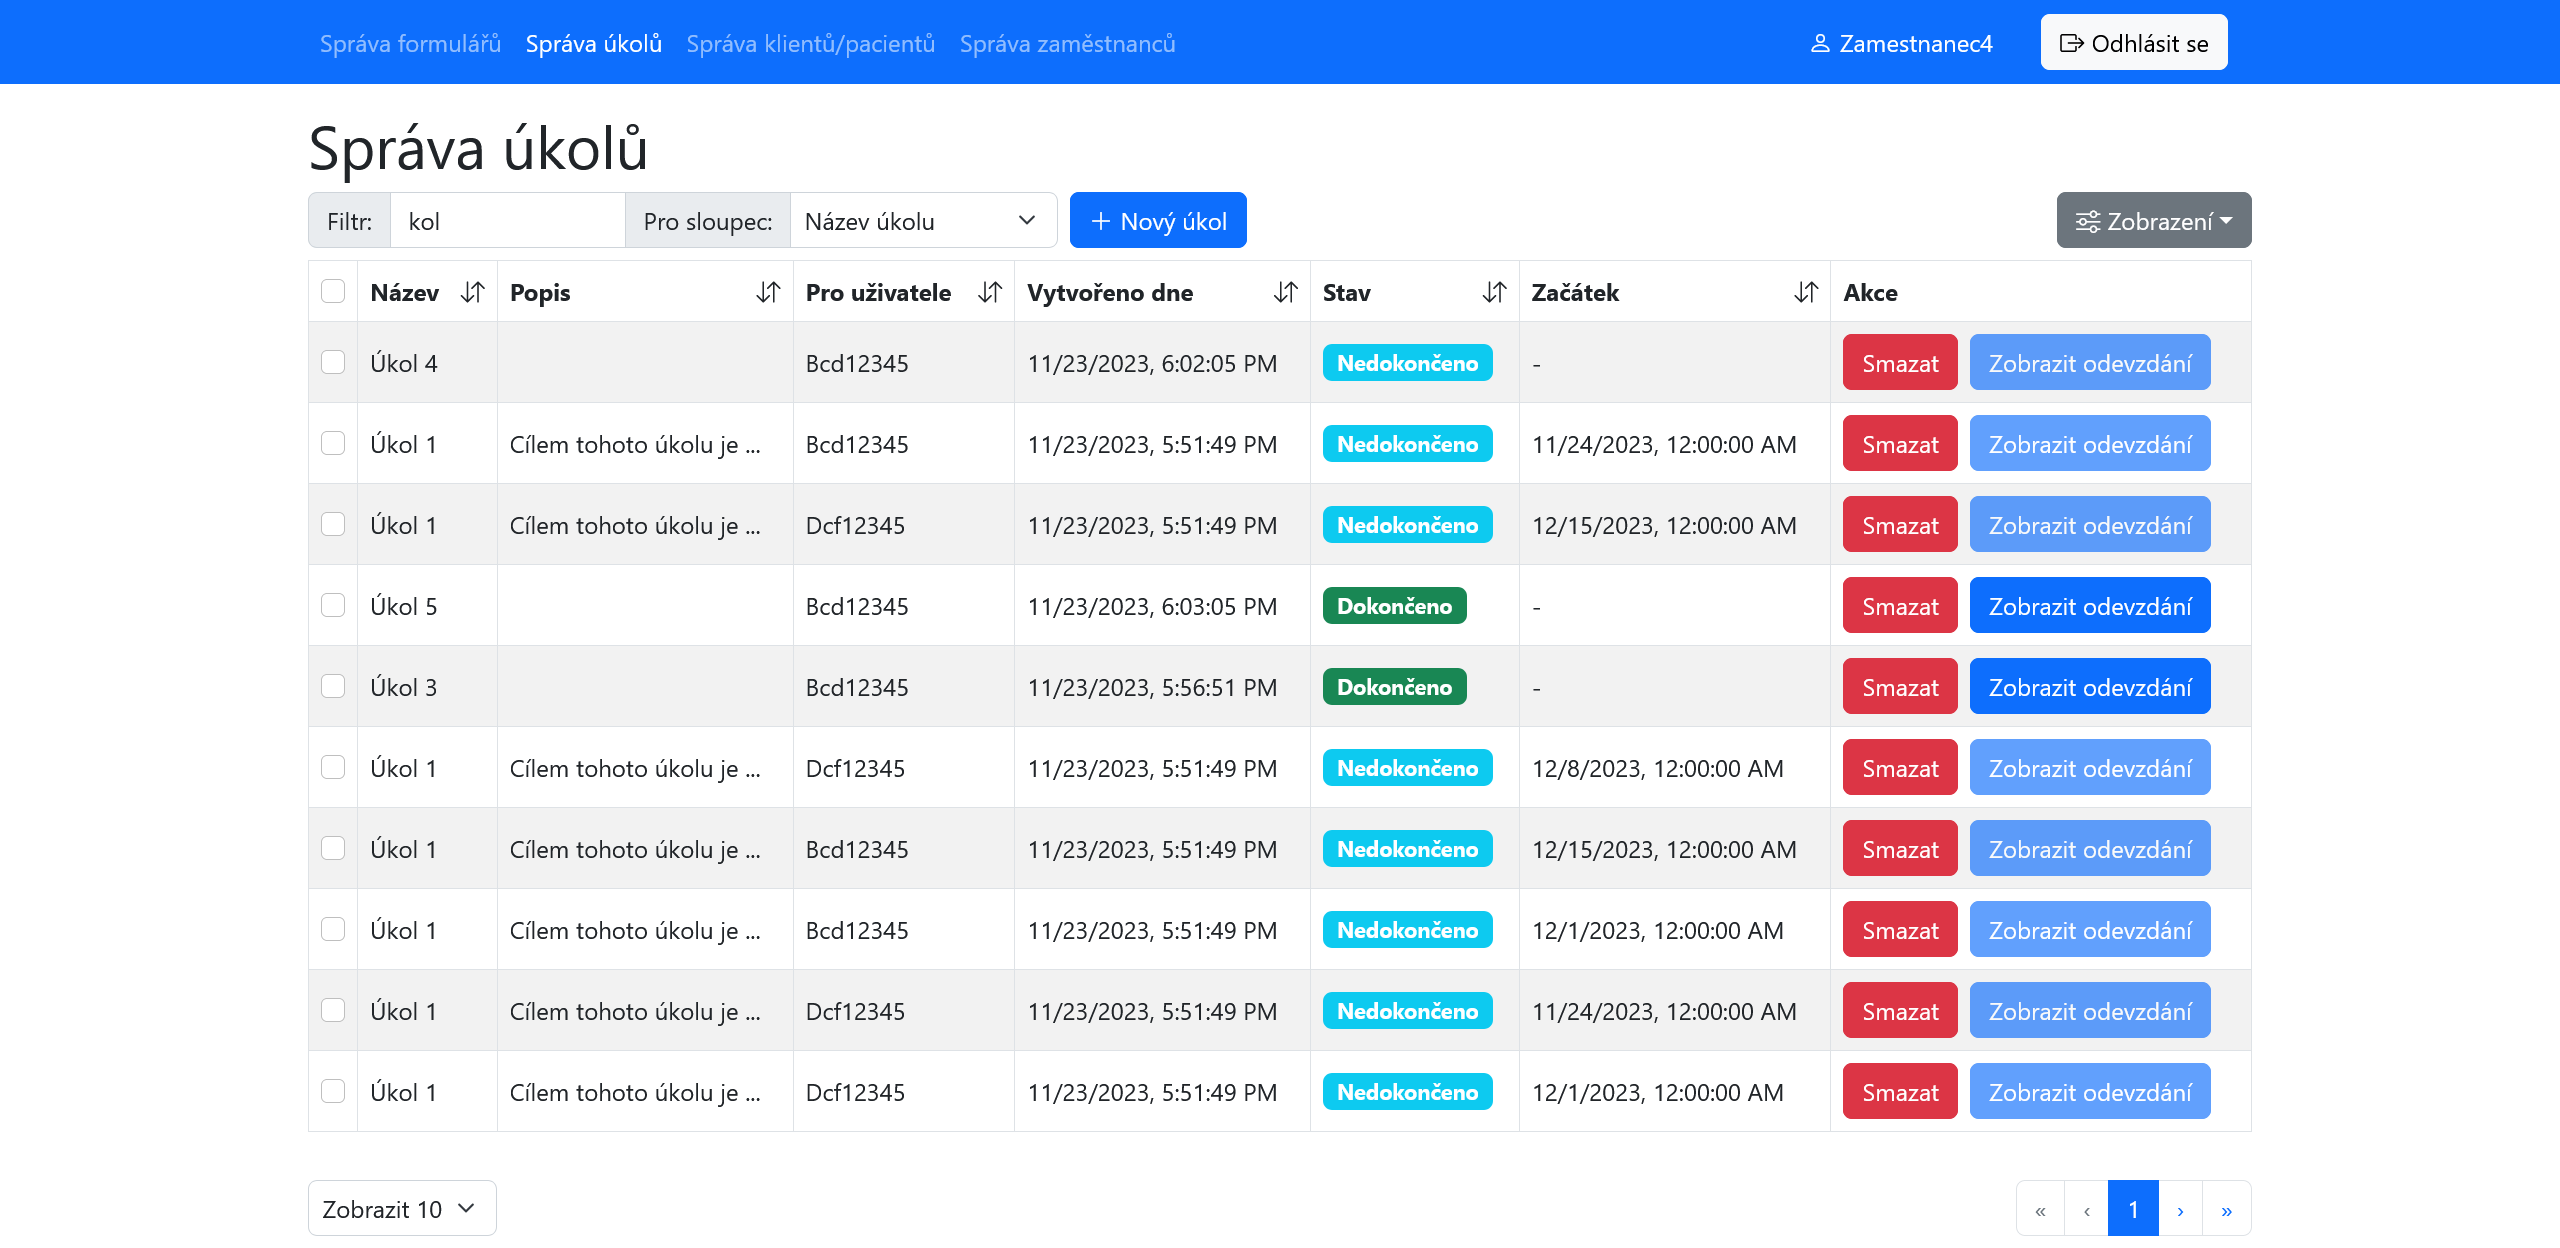
\includegraphics[width=\textwidth]{../img/screenshots/sprava-ukolu}
    \caption{Správa úkolů}\label{fig:sprava-ukolu-screenshot}
\end{figure}

\begin{figure}[H]
    \centering
    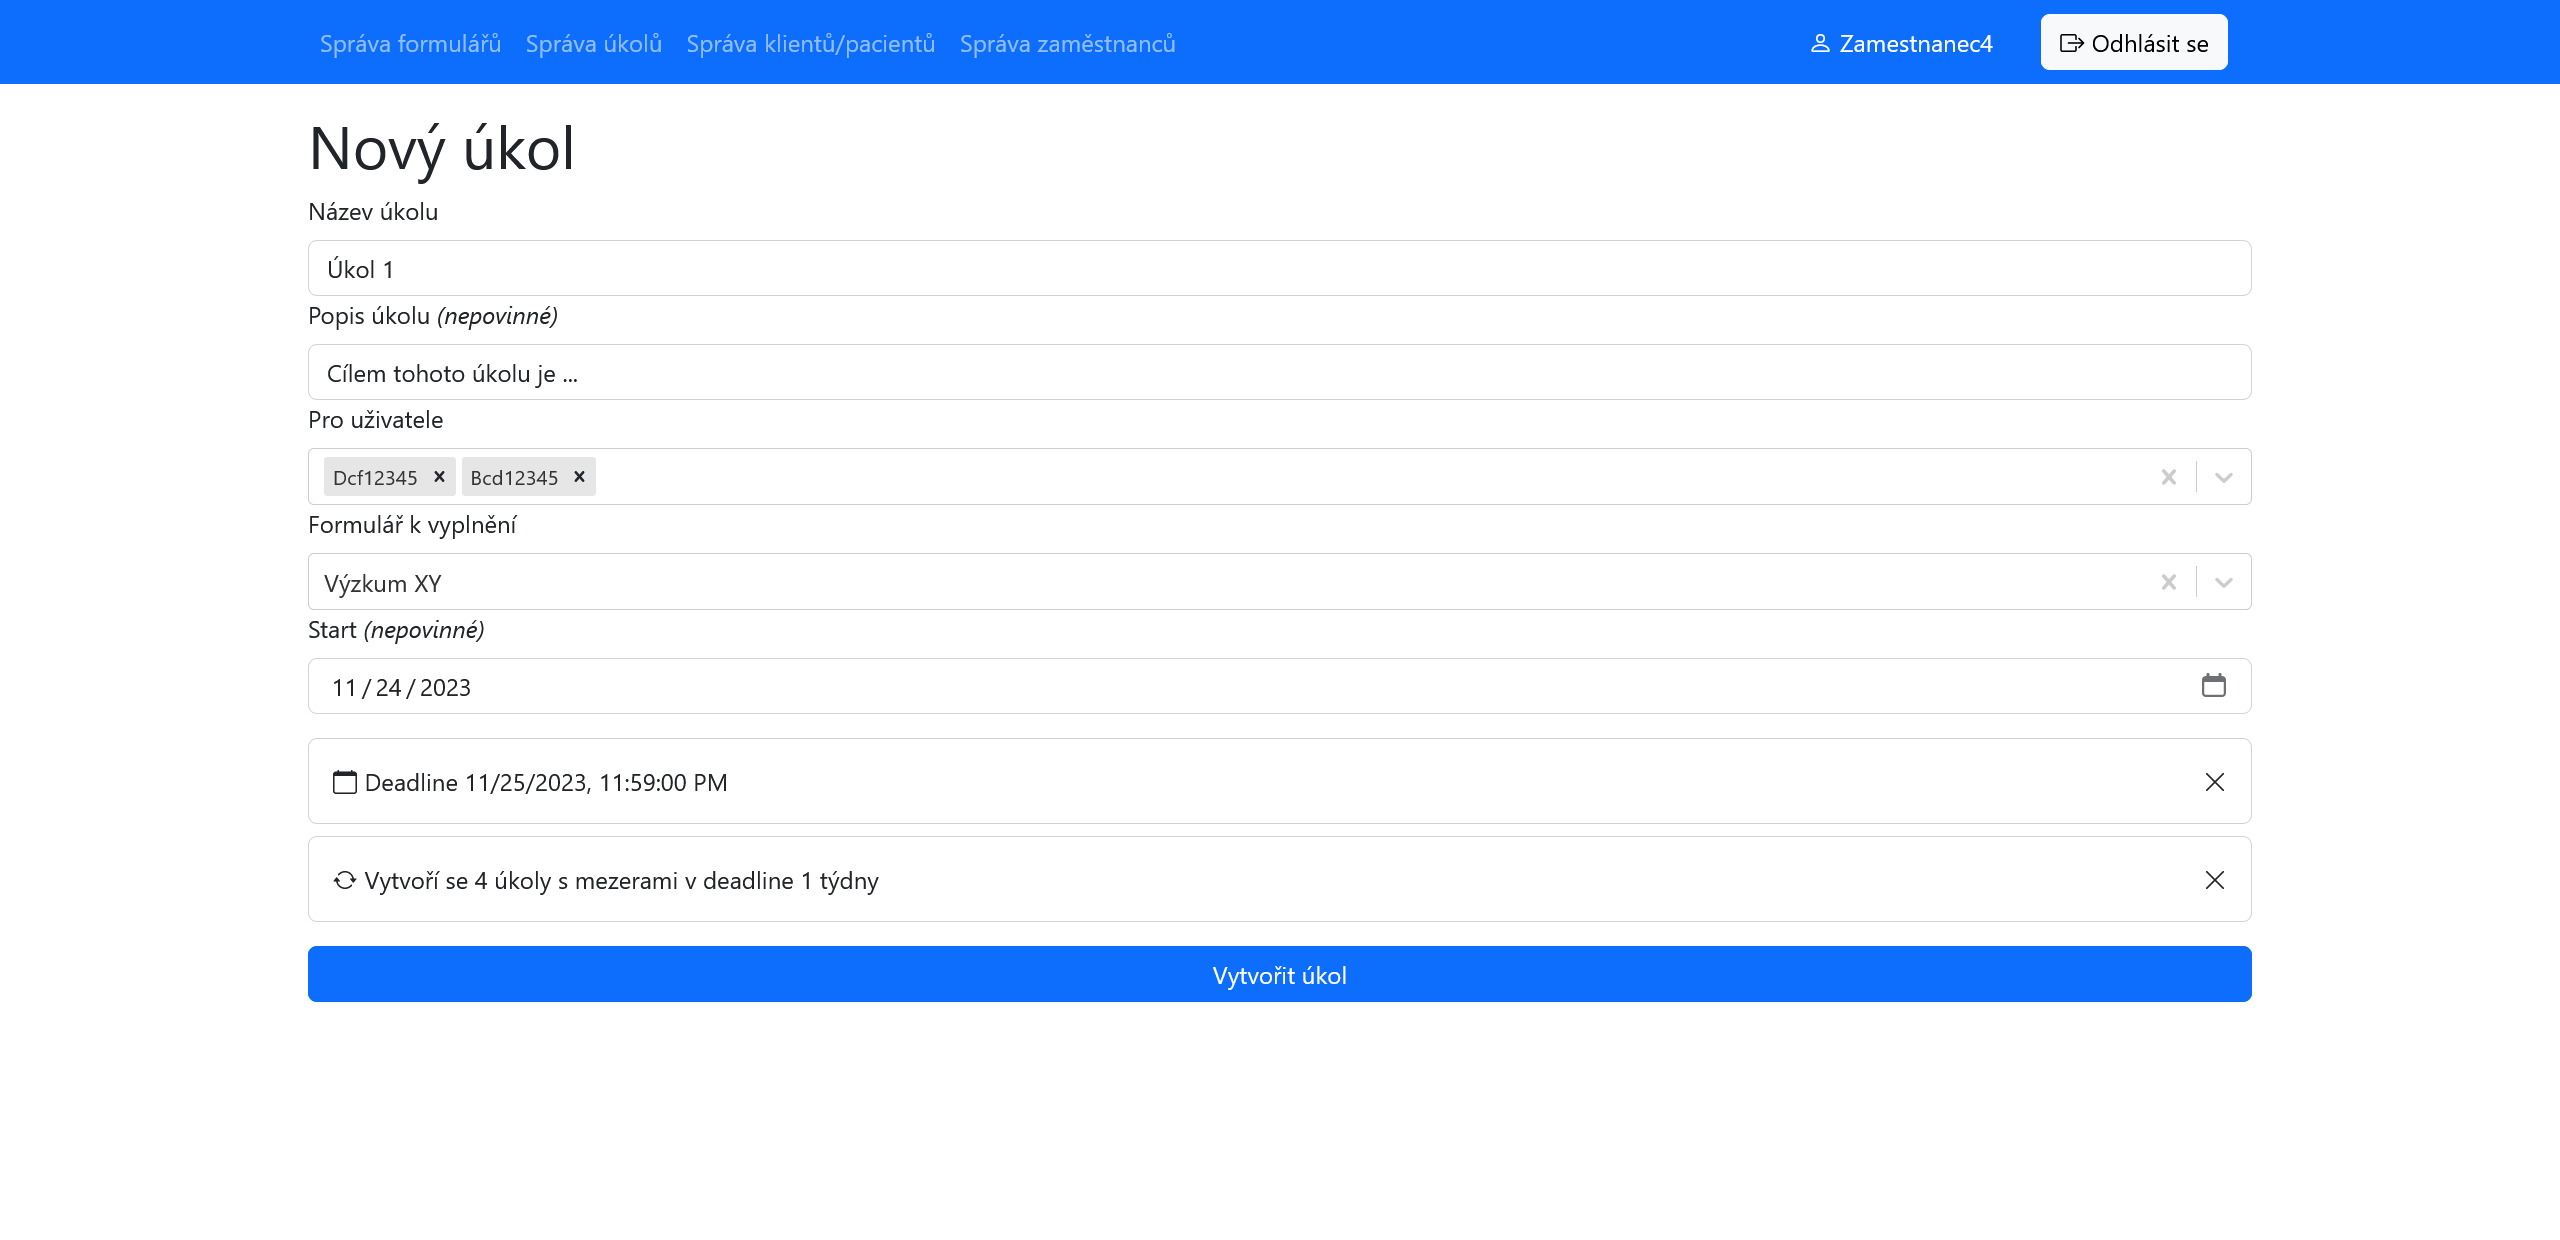
\includegraphics[width=\textwidth]{../img/screenshots/tvorba-ukolu}
    \caption{Tvorba úkolu}\label{fig:tvorba-ukolu-screenshot}
\end{figure}

\begin{figure}[H]
    \centering
    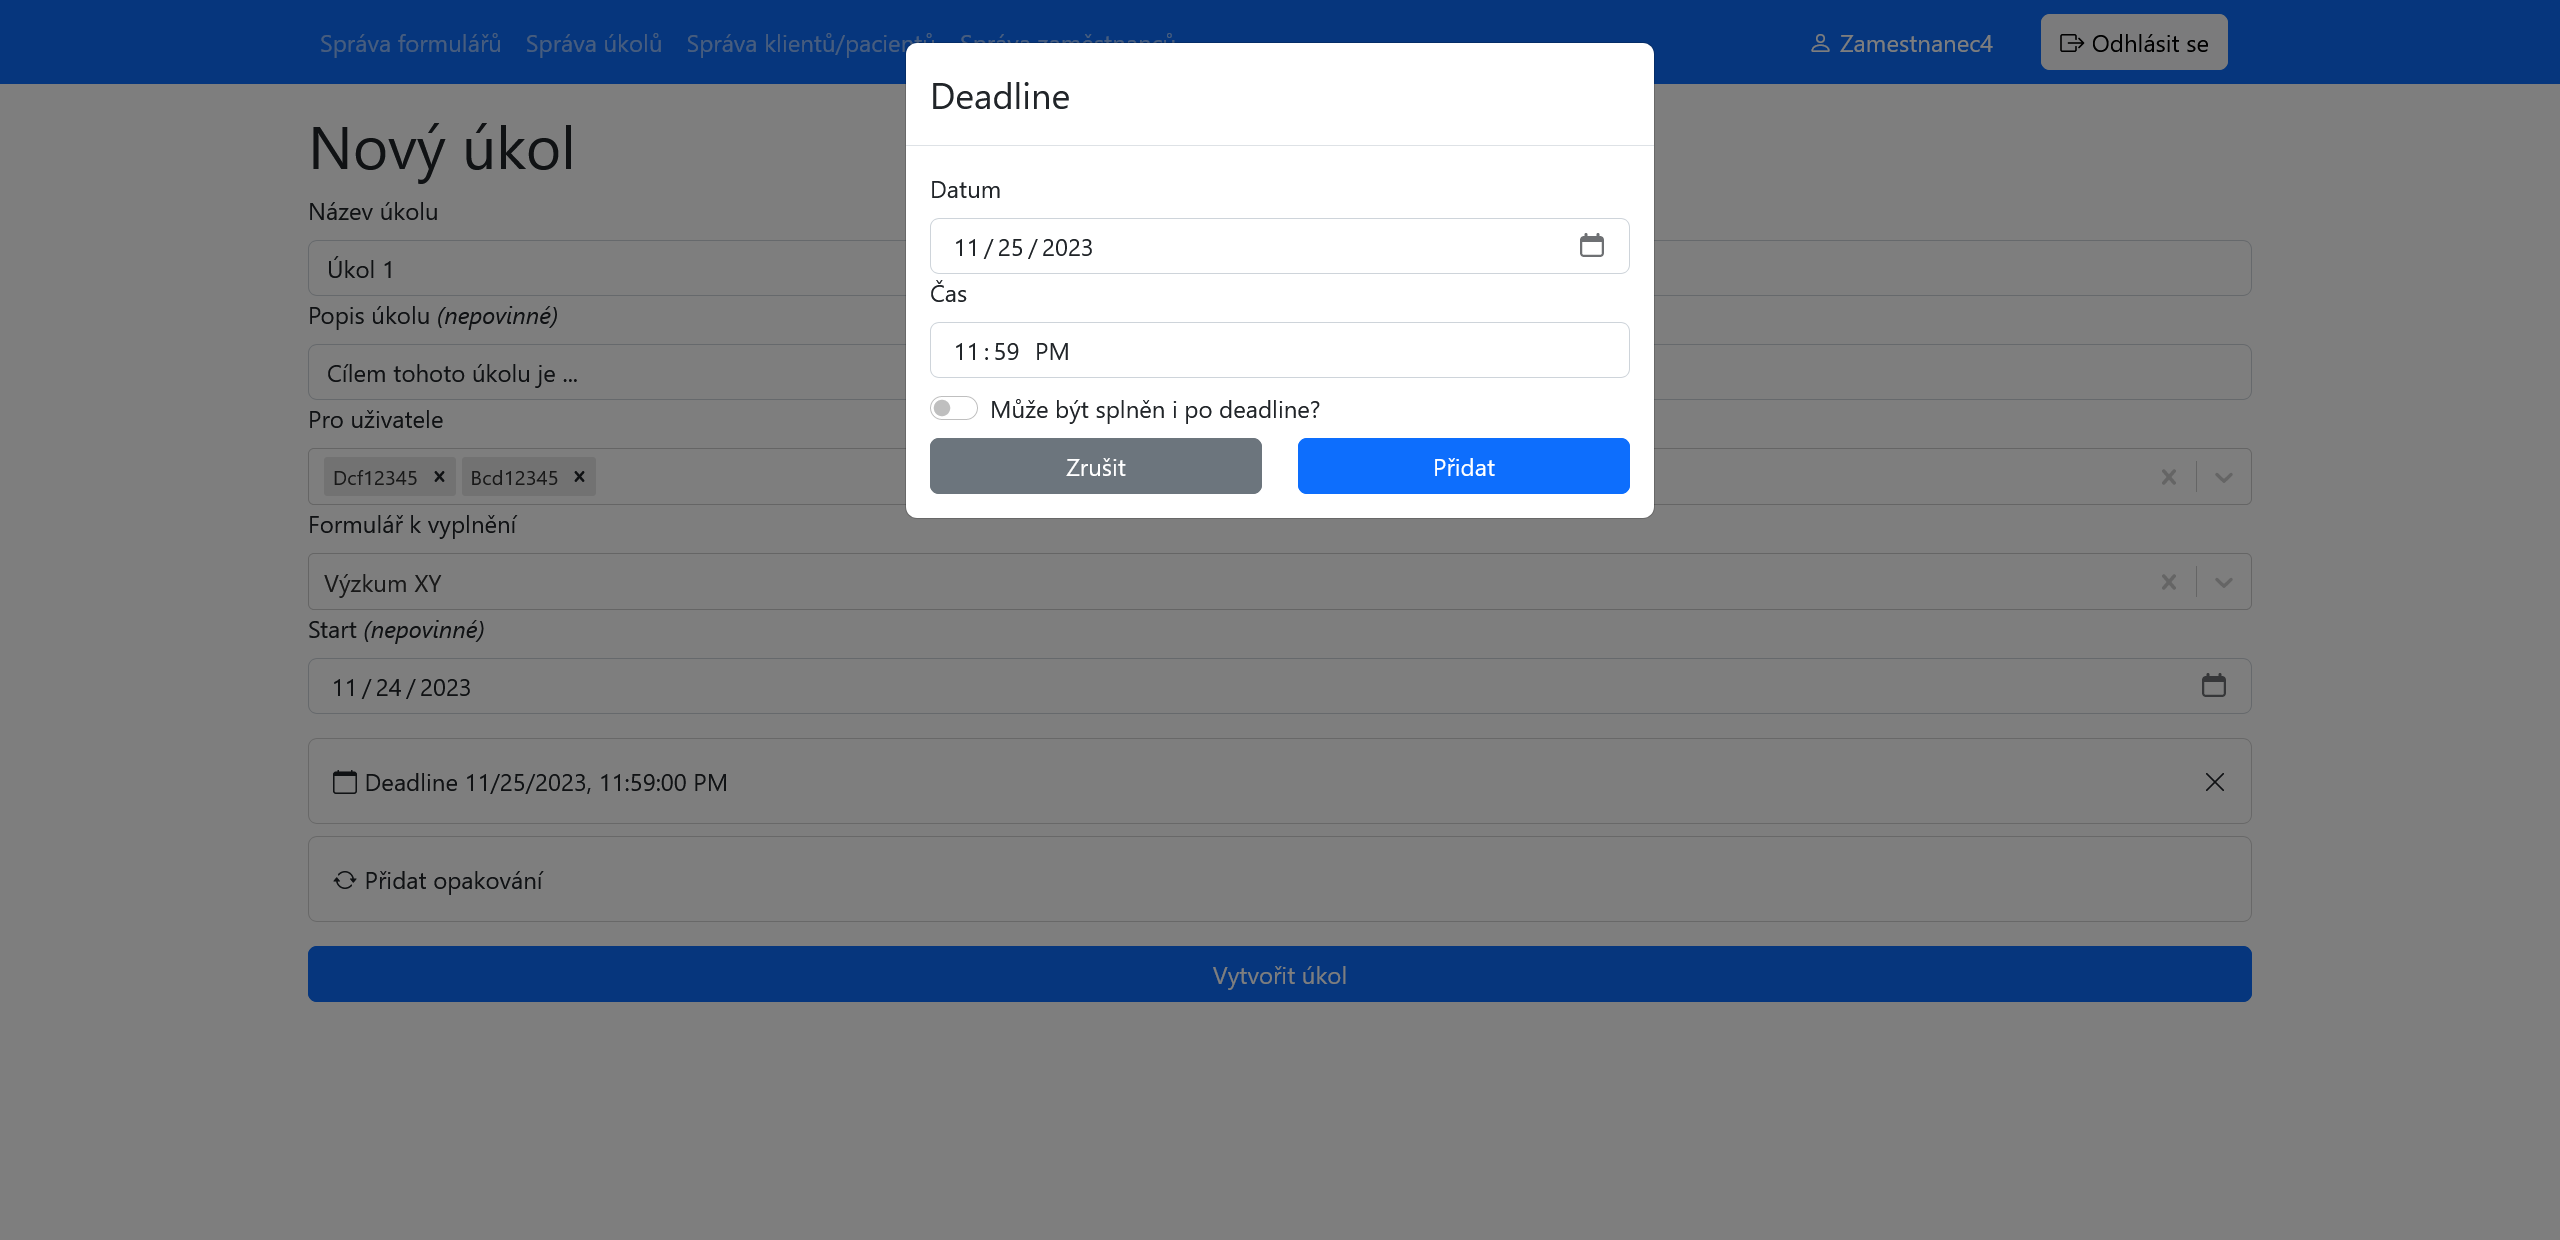
\includegraphics[width=\textwidth]{../img/screenshots/tvorba-ukolu-deadline}
    \caption{Zadávání deadline při tvorbě úkolu}\label{fig:tvorba-ukolu-deadline-screenshot}
\end{figure}

\begin{figure}[H]
    \centering
    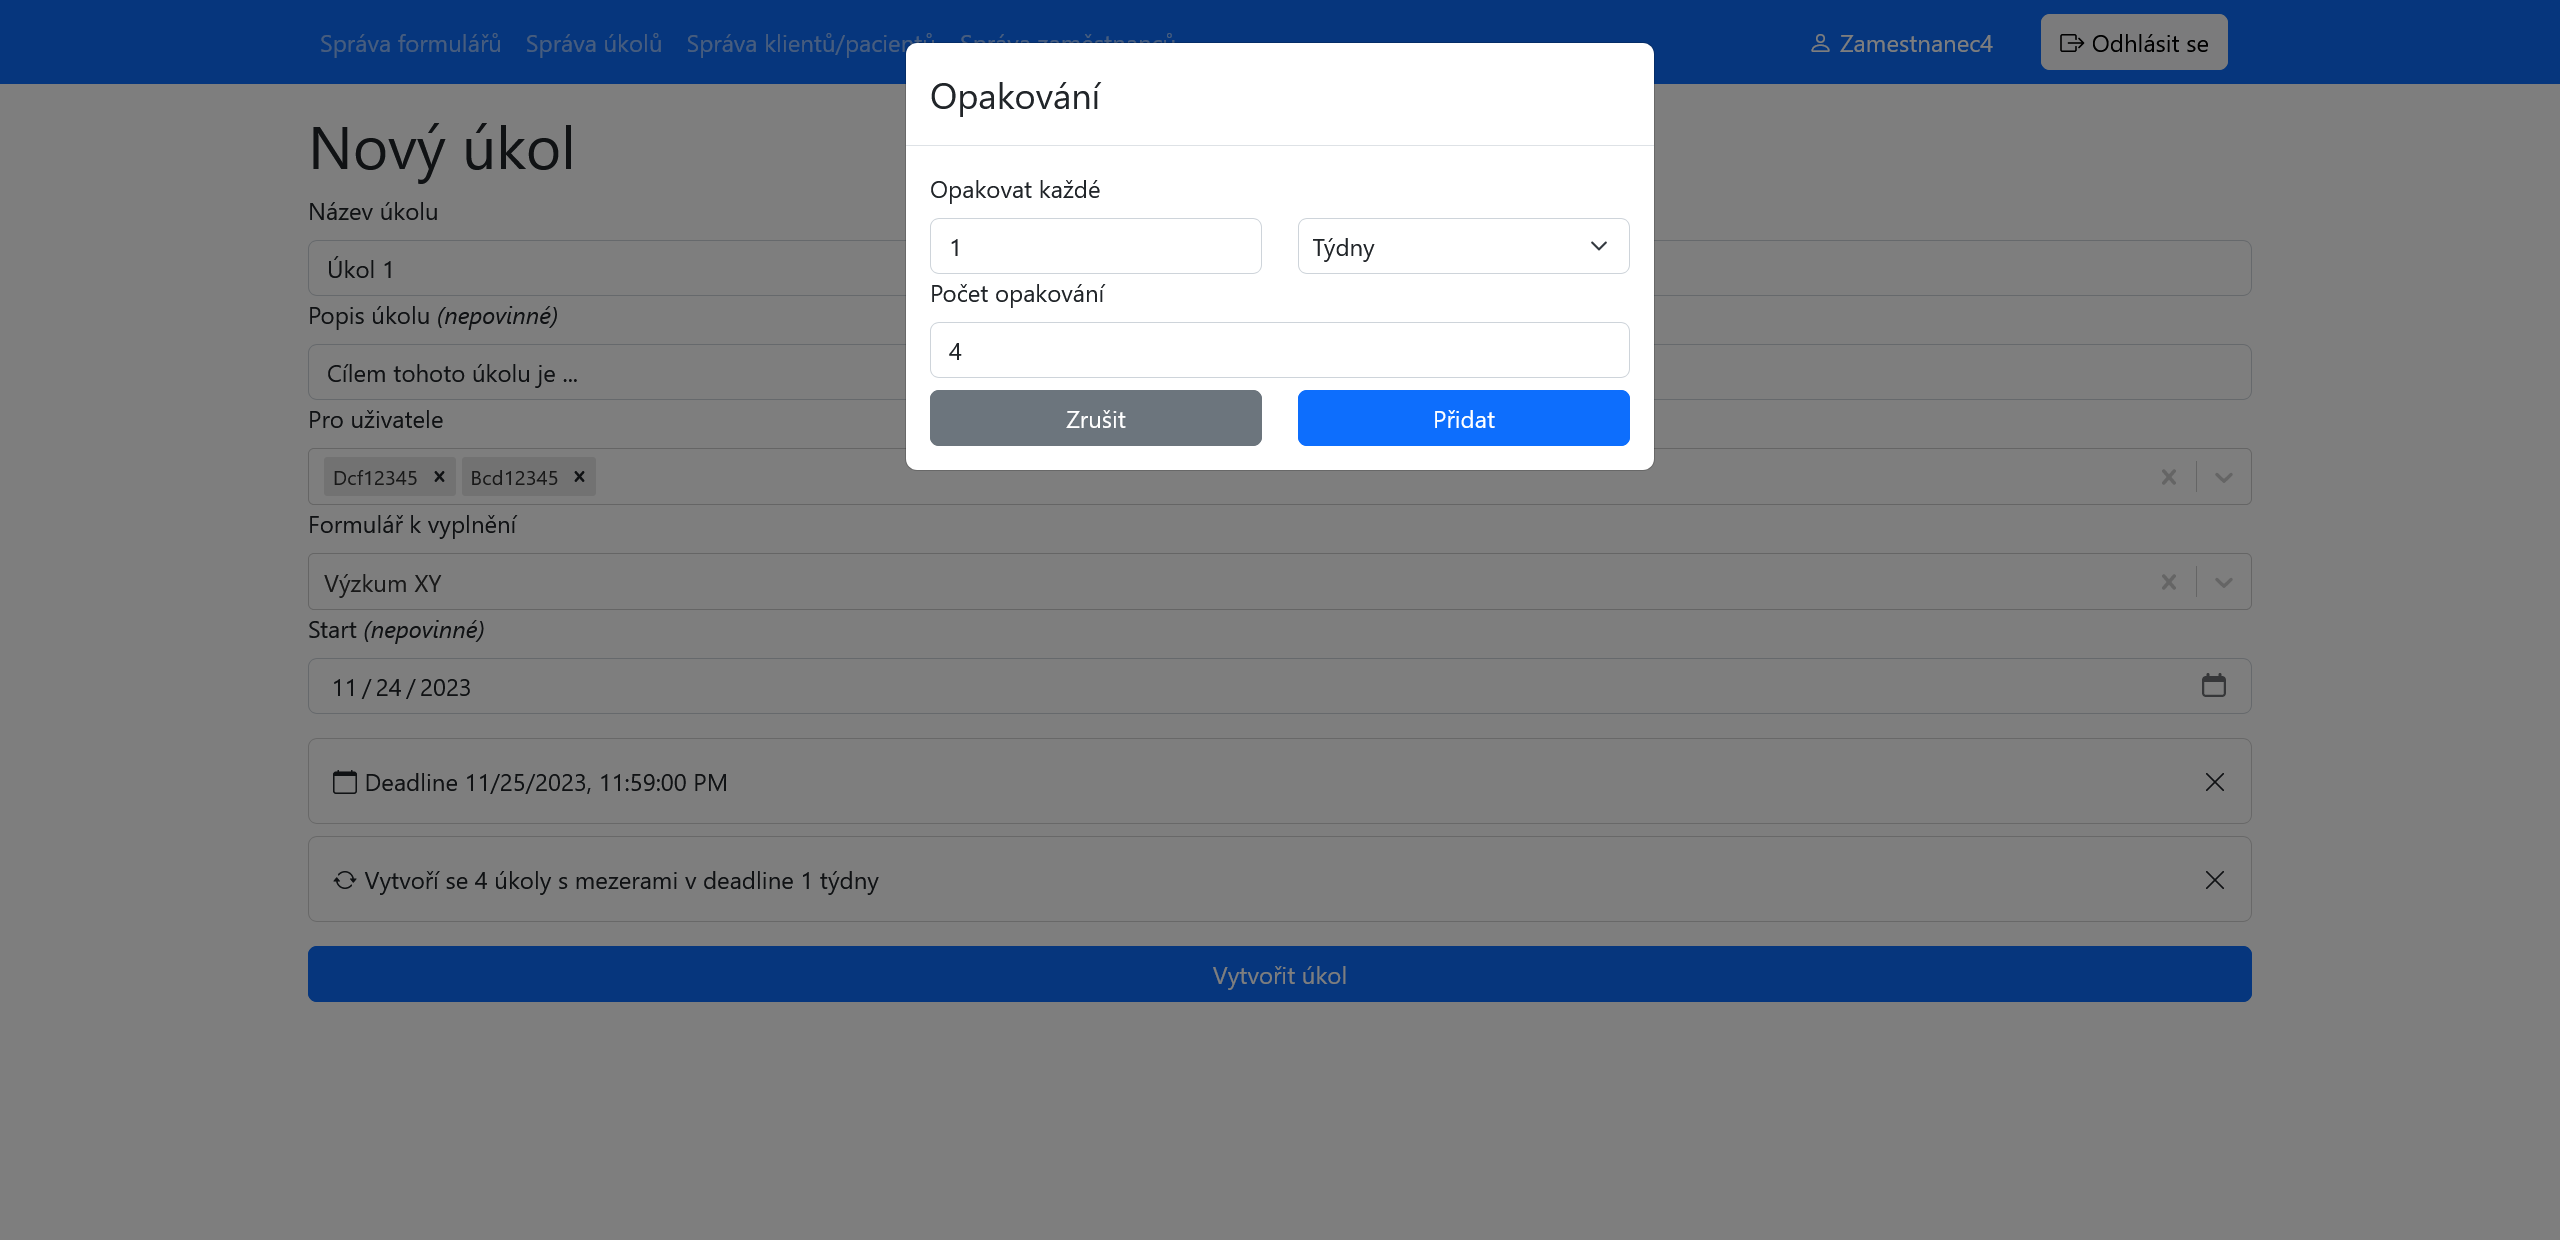
\includegraphics[width=\textwidth]{../img/screenshots/tvorba-ukolu-opakovani}
    \caption{Konfigurace opakování při tvorbě úkolu}\label{fig:tvorba-ukolu-opakovani-screenshot}
\end{figure}

\subsection{Náhled na odevzdání formuláře}\label{subsec:nahled-odevzdani-formulare}

Nyní předpokládejme, že plnitel splnil zadaný úkol.
Zaměstnanec si může zobrazit odevzdání formuláře pomocí tlačítka \uv{Zobrazit odevzdání} v sekci \uv{Správa úkolů} (Obr.~\ref{fig:sprava-ukolu-screenshot}).
Náhled na odevzdání obsahuje metadata vyplnění formuláře a vyplněný formulář (Obr.~\ref{fig:nahled-odevzdani-zamestnanec-screenshot}).
Náhled na odevzdaní zobrazuje i skryté prvky formuláře a jejich hodnoty.

\begin{figure}[H]
    \centering
    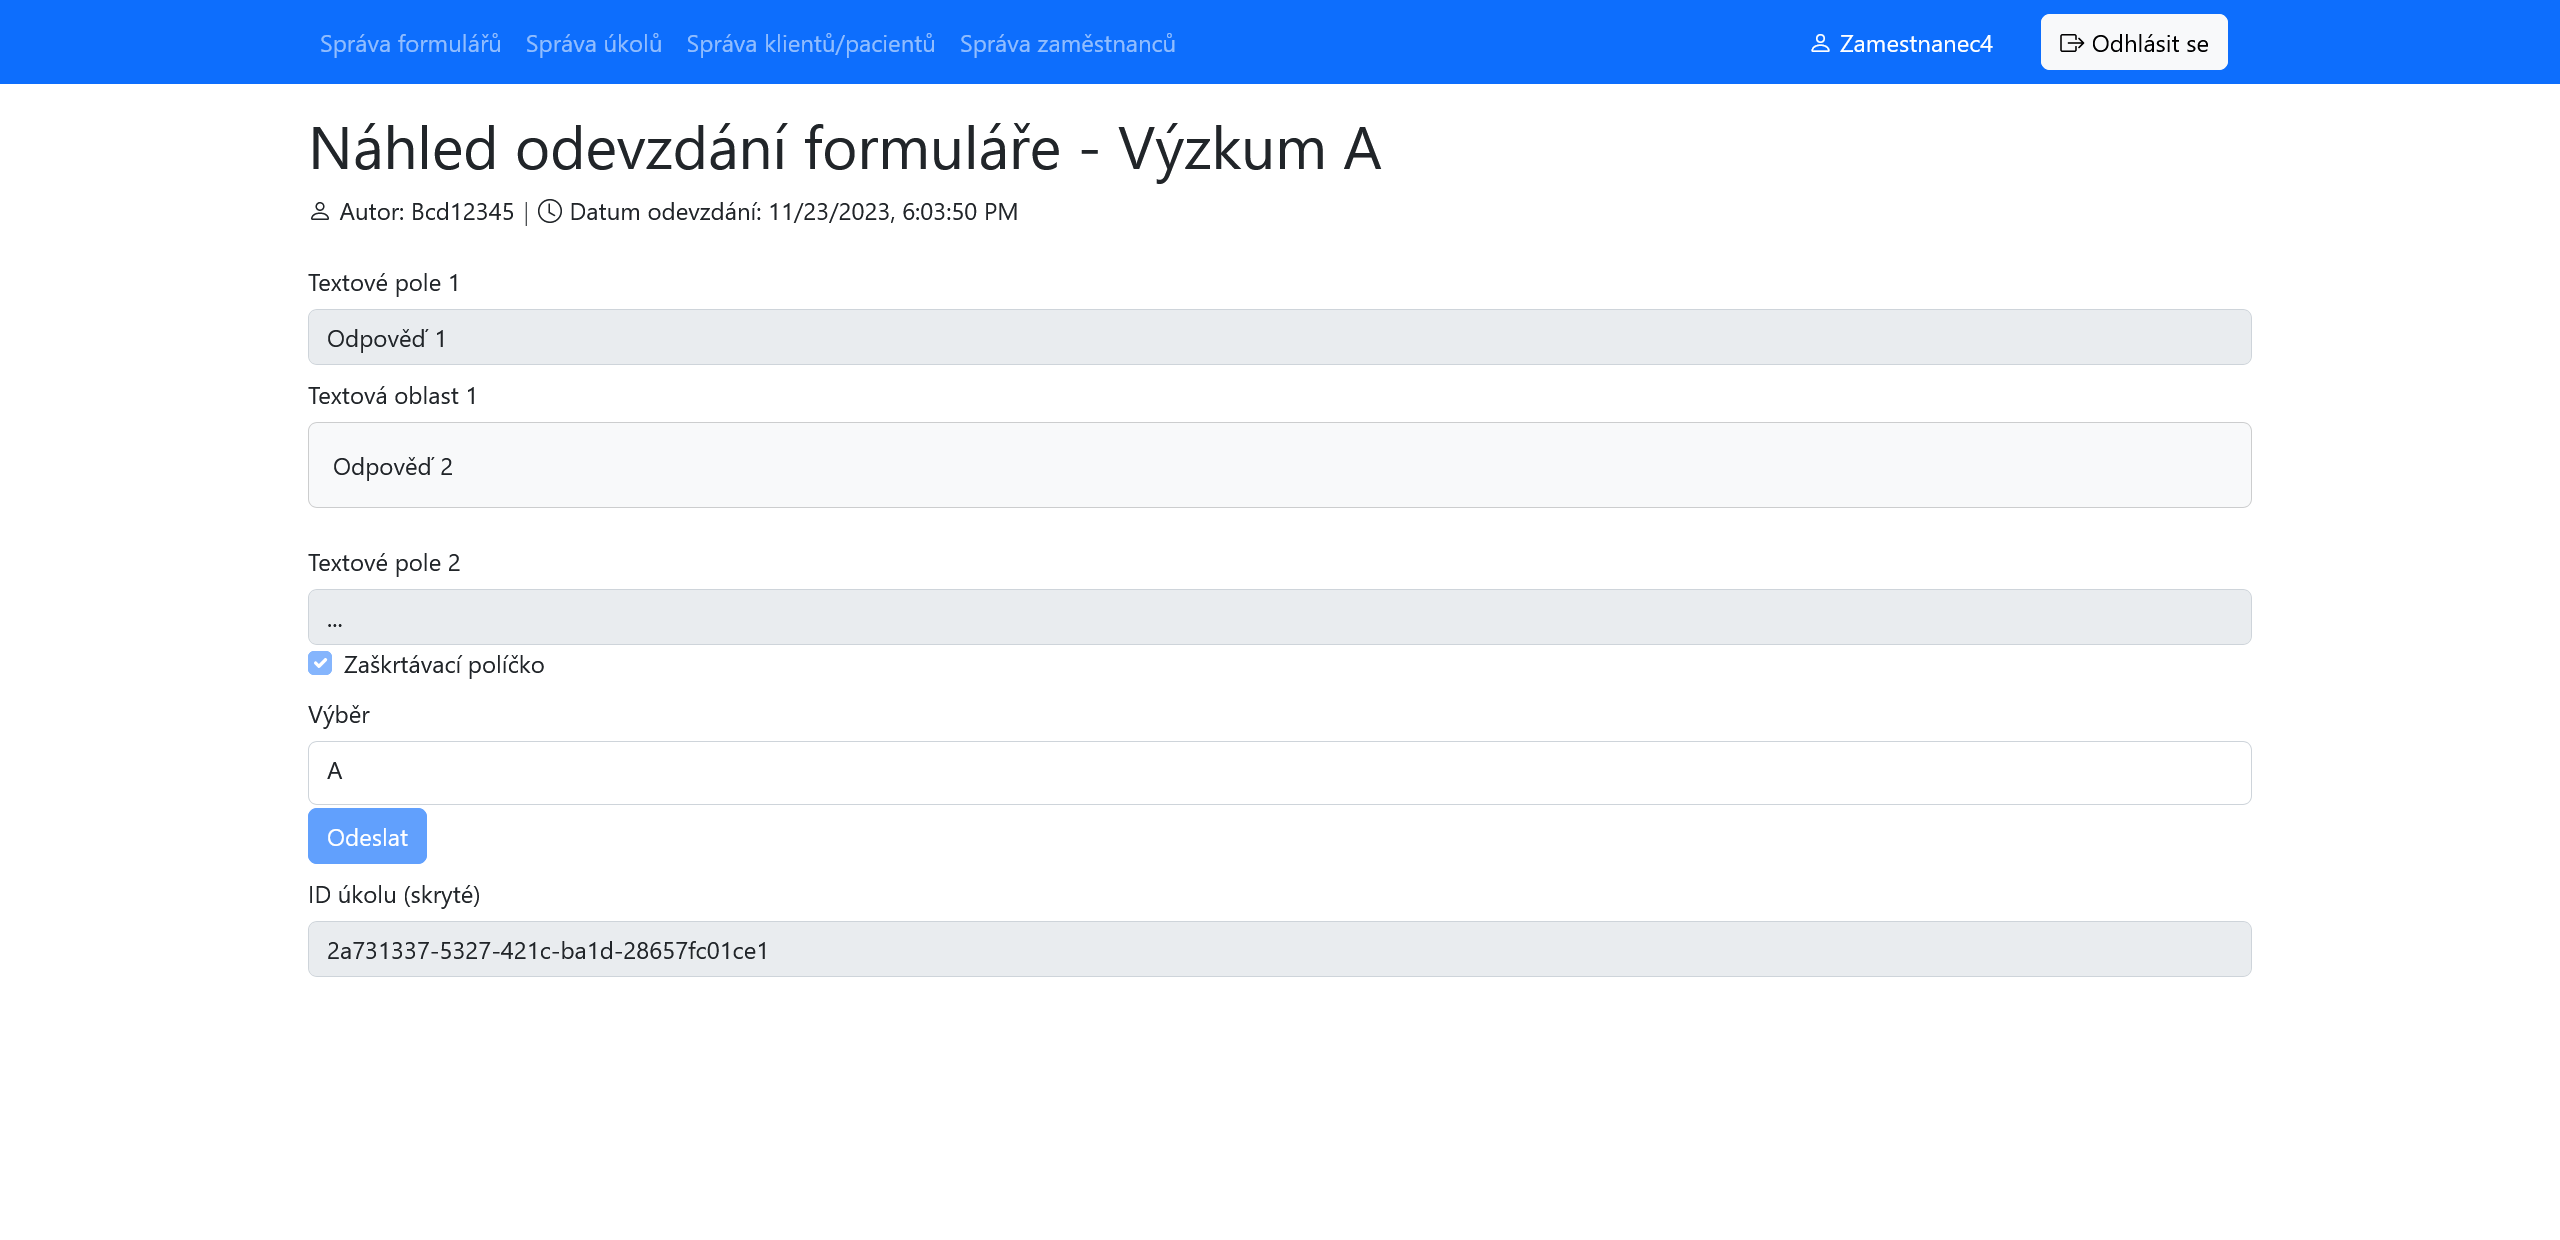
\includegraphics[width=\textwidth]{../img/screenshots/nahled-odevzdani-zamestnanec}
    \caption{Náhled na jednotlivé odevzdání formuláře}\label{fig:nahled-odevzdani-zamestnanec-screenshot}
\end{figure}

Můžeme také zobrazit všechna odevzdání formuláře formou tabulky pomocí tlačítka \uv{Zobrazit všechna odevzdání} v sekci \uv{Správa formulářů} (Obr.~\ref{fig:sprava-formularu-screenshot}).
Tato stránka obsahuje seznam všech odevzdání formuláře (Obr.~\ref{fig:nahled-vsechna-odevzdani-zamestnanec-screenshot}), které lze řadit, filtrovat a následně i exportovat do souboru.
Stránka také umožňuje vytvořit základní vizualizace sesbíraných dat, které lze zobrazit stisknutím tlačítka \uv{Vizualizovat frekvence hodnot} (Obr.~\ref{fig:nahled-vsechna-odevzdani-vizualizace-zamestnanec-screenshot}).
Pokročilejší analýzy a vizualizace dat je možno provádět specializovaným softwarem, který je schopen zpracovat exportovaná data.

\begin{figure}[H]
    \centering
    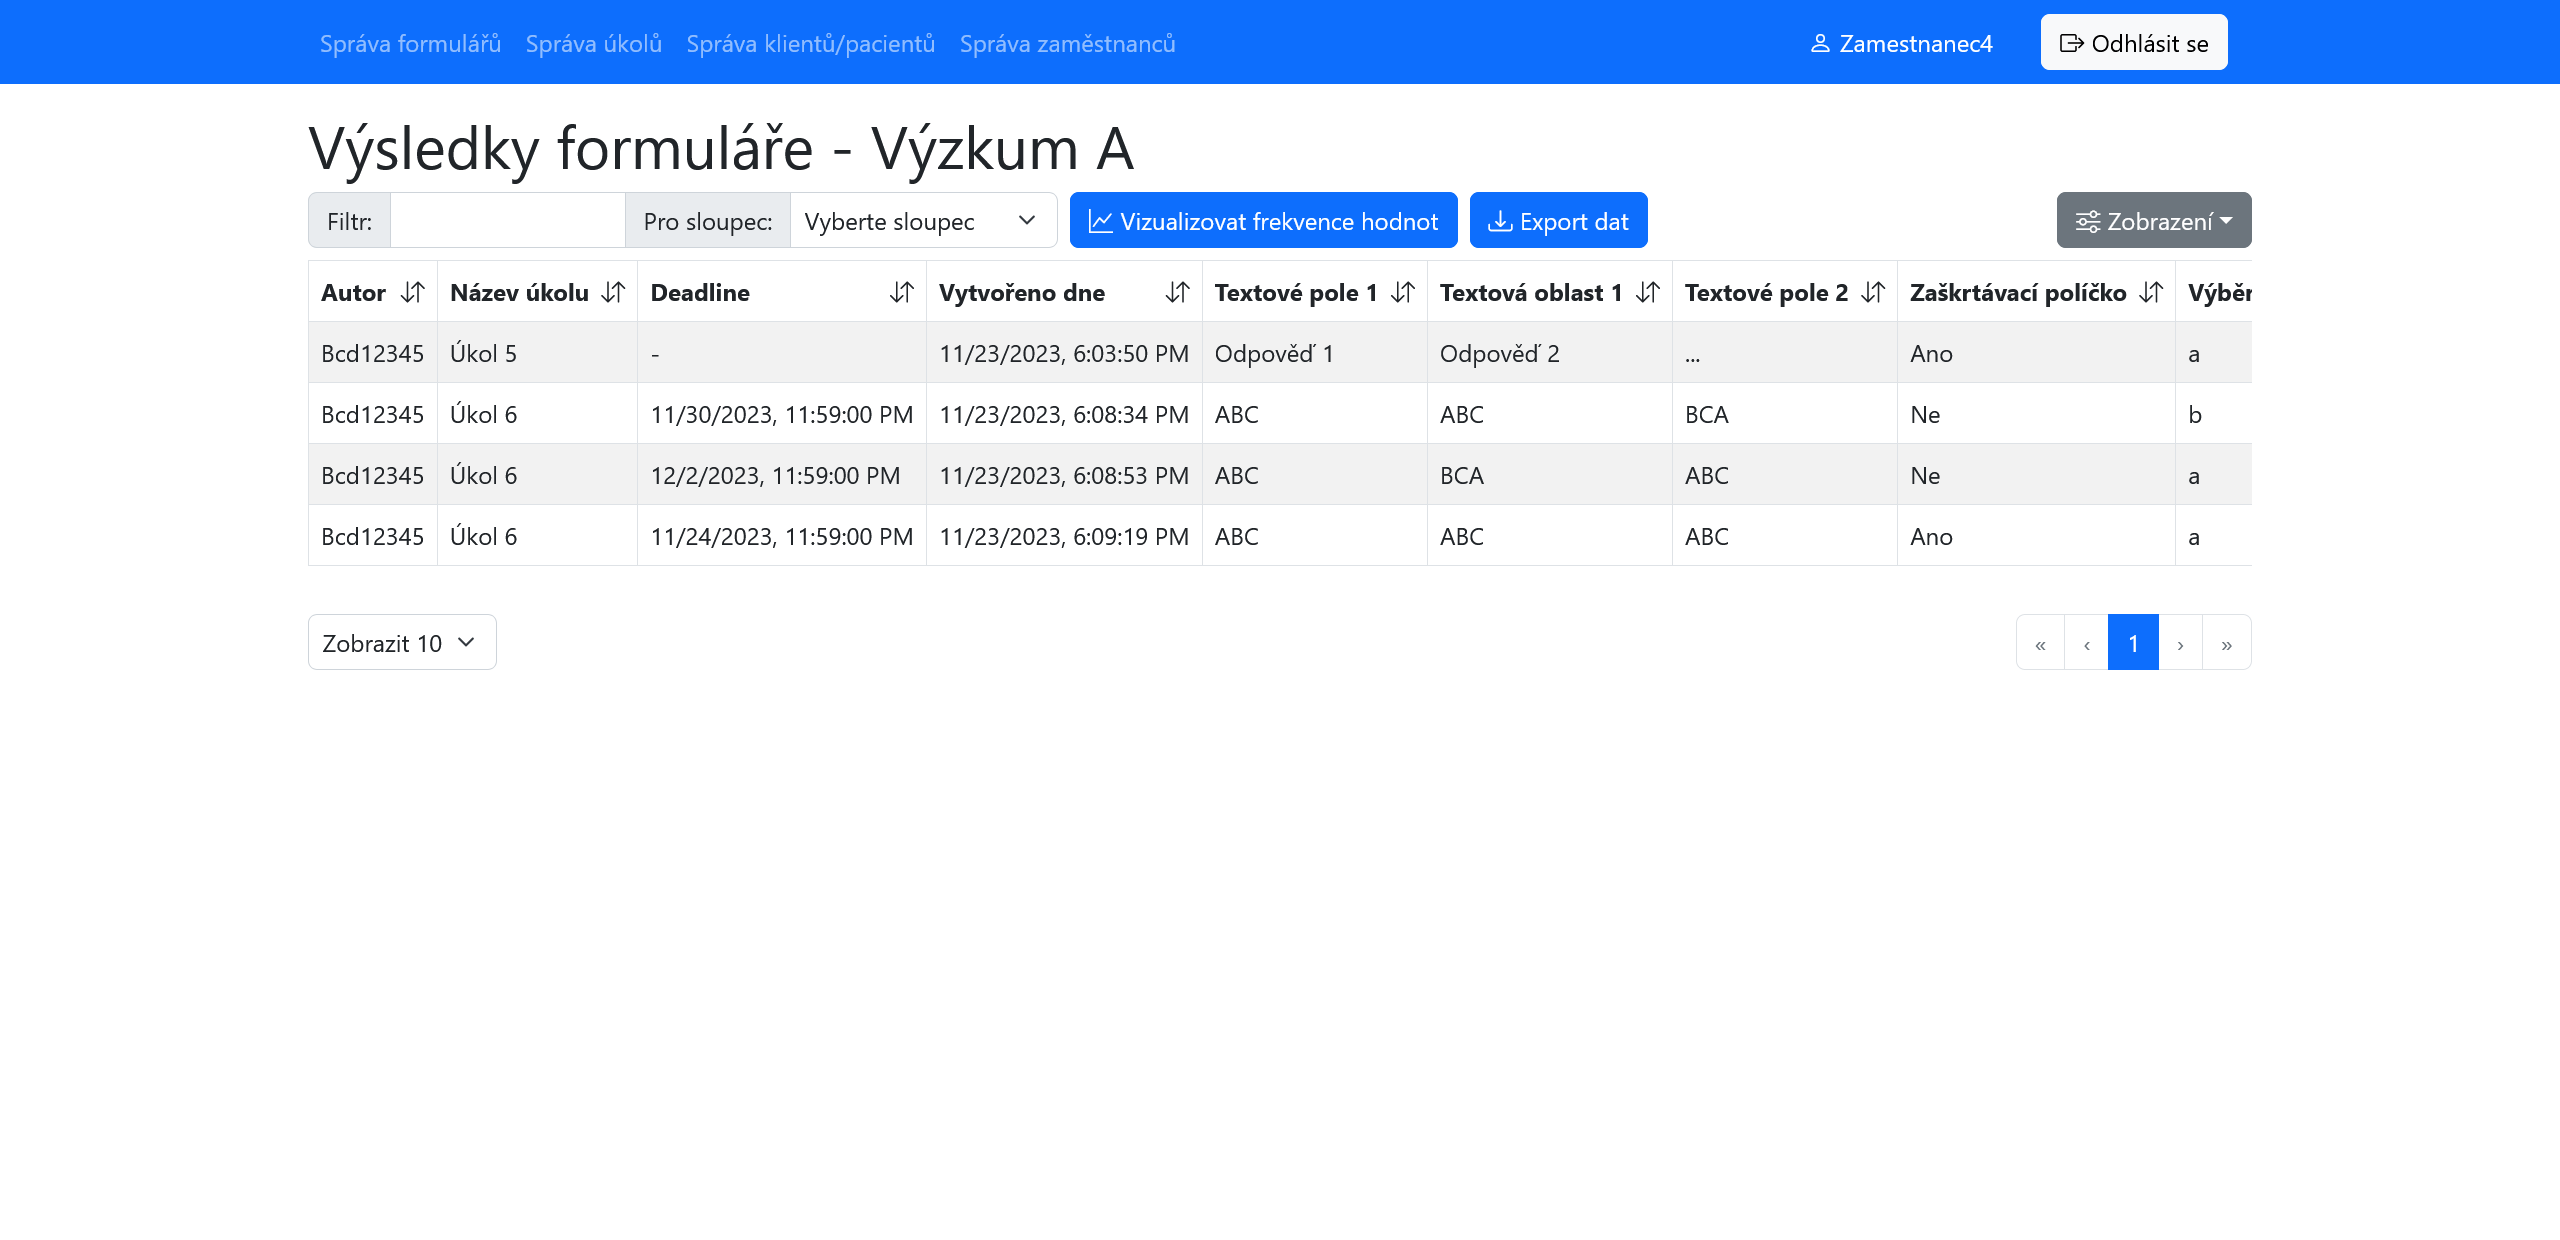
\includegraphics[width=\textwidth]{../img/screenshots/vysledky-formulare}
    \caption{Náhled na všechna odevzdání formuláře}\label{fig:nahled-vsechna-odevzdani-zamestnanec-screenshot}
\end{figure}

\begin{figure}[H]
    \centering
    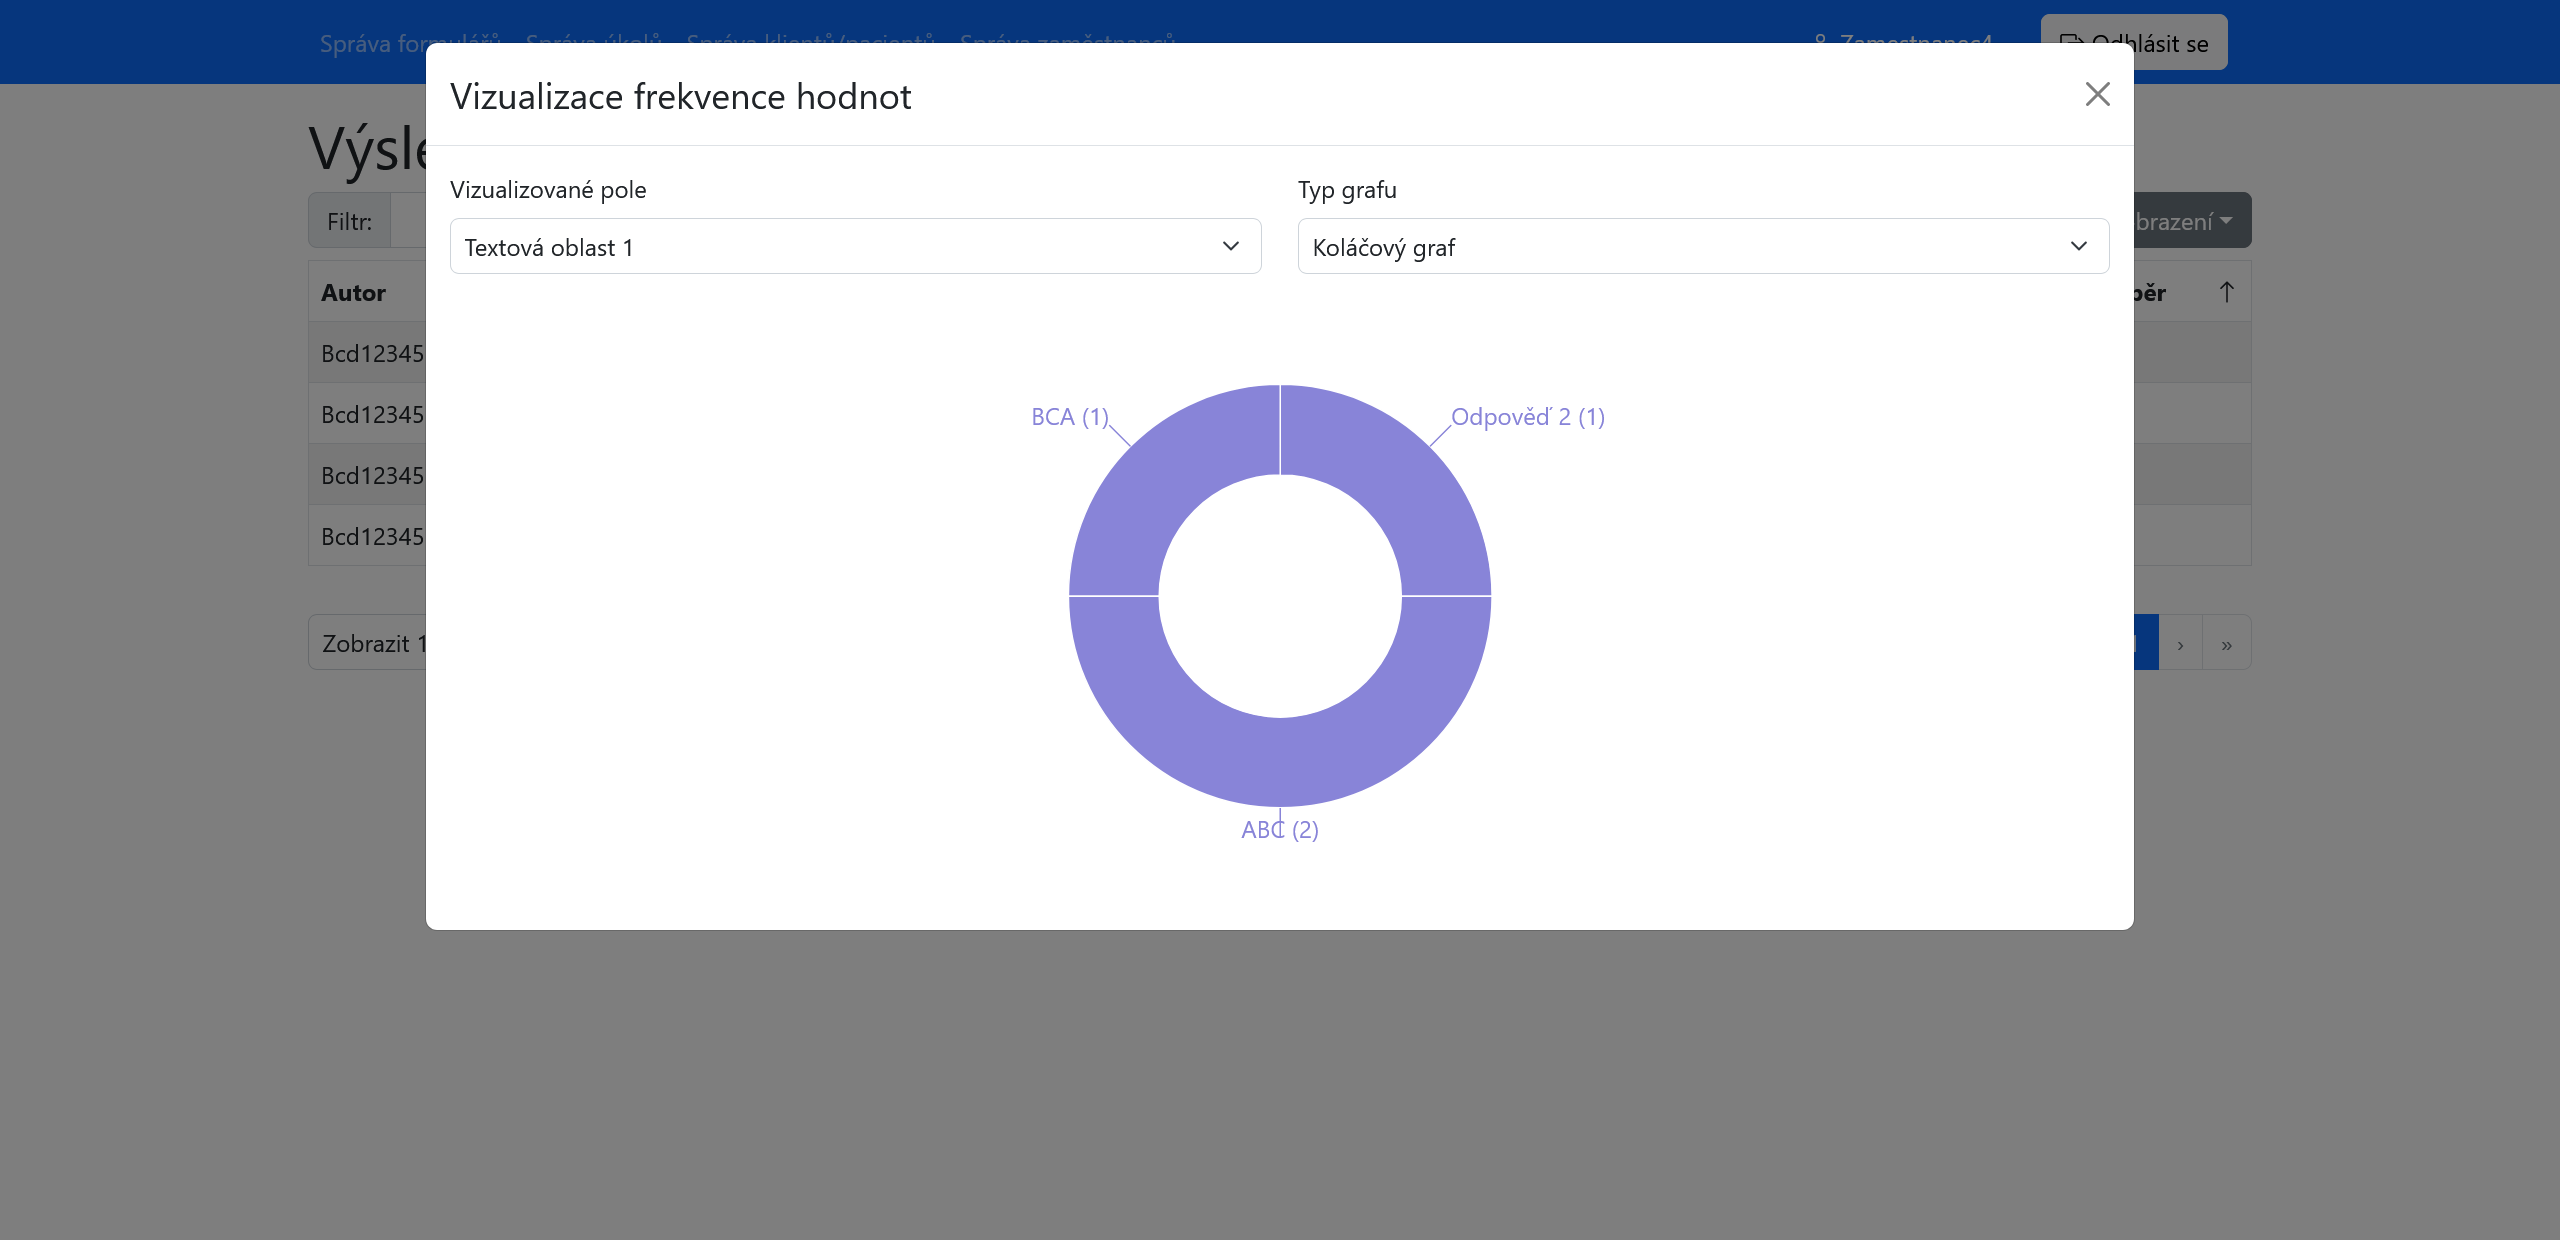
\includegraphics[width=\textwidth]{../img/screenshots/vysledky-formulare-vizualizace}
    \caption{Vizualizace odevzdání formuláře}\label{fig:nahled-vsechna-odevzdani-vizualizace-zamestnanec-screenshot}
\end{figure}

\subsection{Správa účtů}\label{subsec:sprava-uctu}

Zaměstnanec může tvořit účty pro další zaměstnance.
Pokud má zaměstnanec roli \uv{Správce dotazníků}, tak může tvořit účty pro další zaměstnance s rolí \uv{Správce dotazníků} nebo \uv{Zadavatel dotazníků}.
Pokud má zaměstnanec roli \uv{Zadavatel dotazníků}, tak může tvořit účty pro další zaměstnance s rolí \uv{Zadavatel dotazníků}.
Pohled zaměstnance s rolí \uv{Správce dotazníků} je zobrazen na obrázku~\ref{fig:sprava-zamestnancu-screenshot}.

\begin{figure}[H]
    \centering
    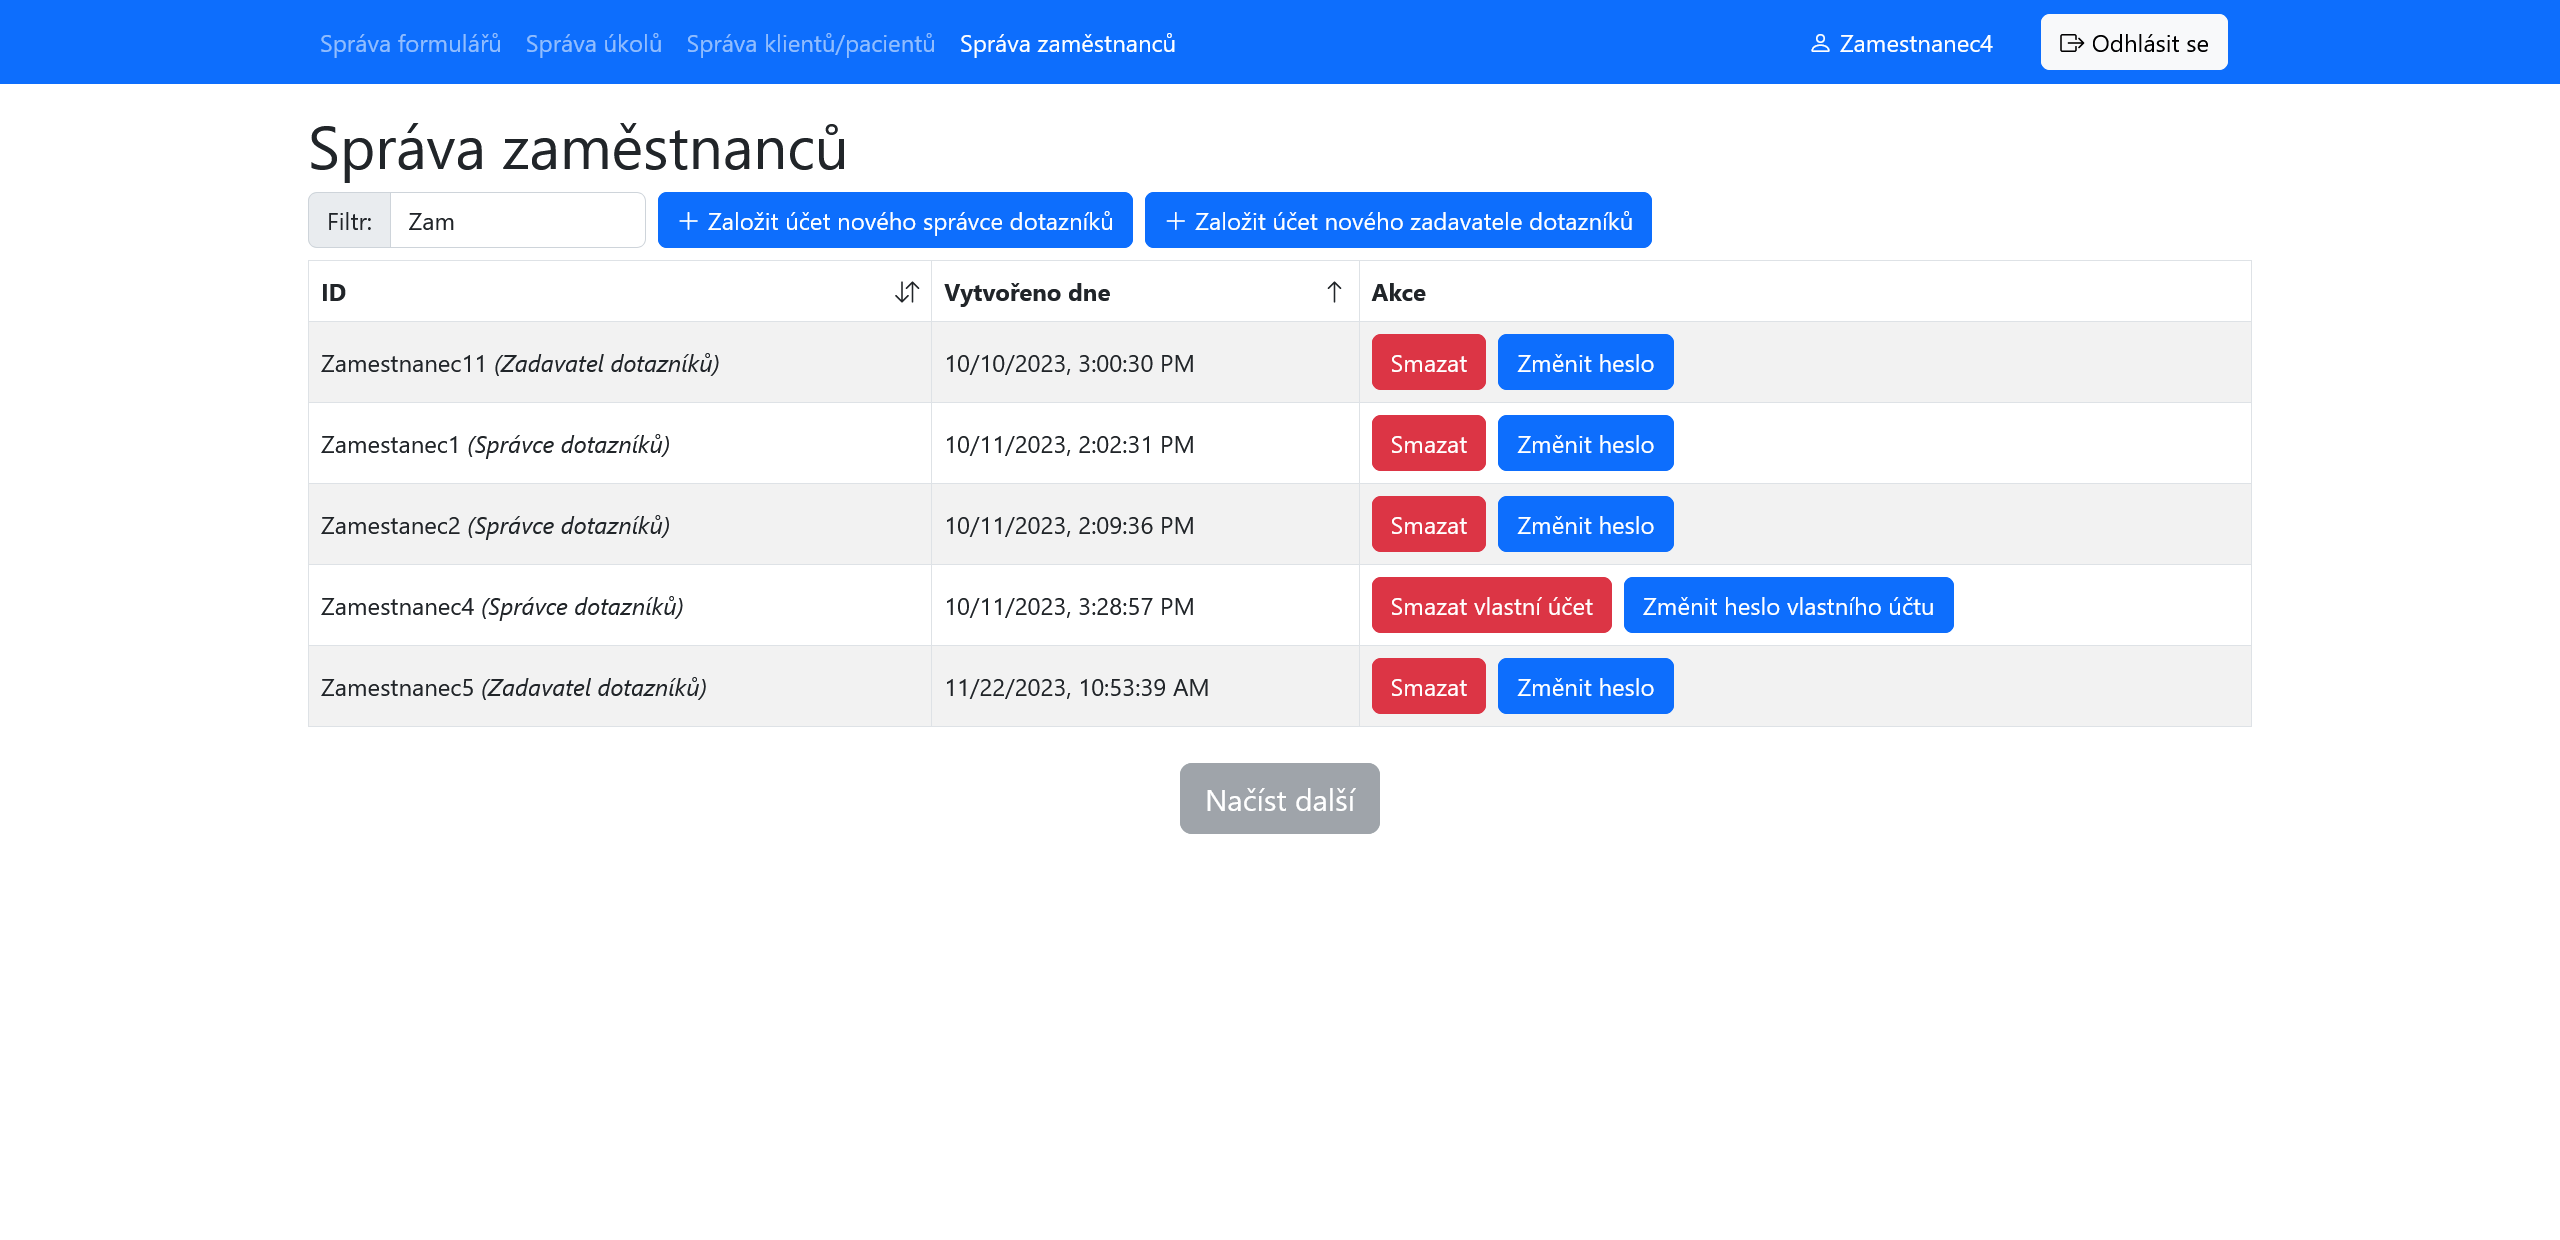
\includegraphics[width=\textwidth]{../img/screenshots/sprava-zamestnancu}
    \caption{Správa zaměstnaneckých účtů}\label{fig:sprava-zamestnancu-screenshot}
\end{figure}

Zaměstnanec si může zobrazit detail svého účtu (Obr.~\ref{fig:zmena-hesla-zamestnanec}) kliknutím na své ID v pravém horním rohu aplikace.
V detailu účtu může zaměstnanec změnit své heslo.

\begin{figure}[H]
    \centering
    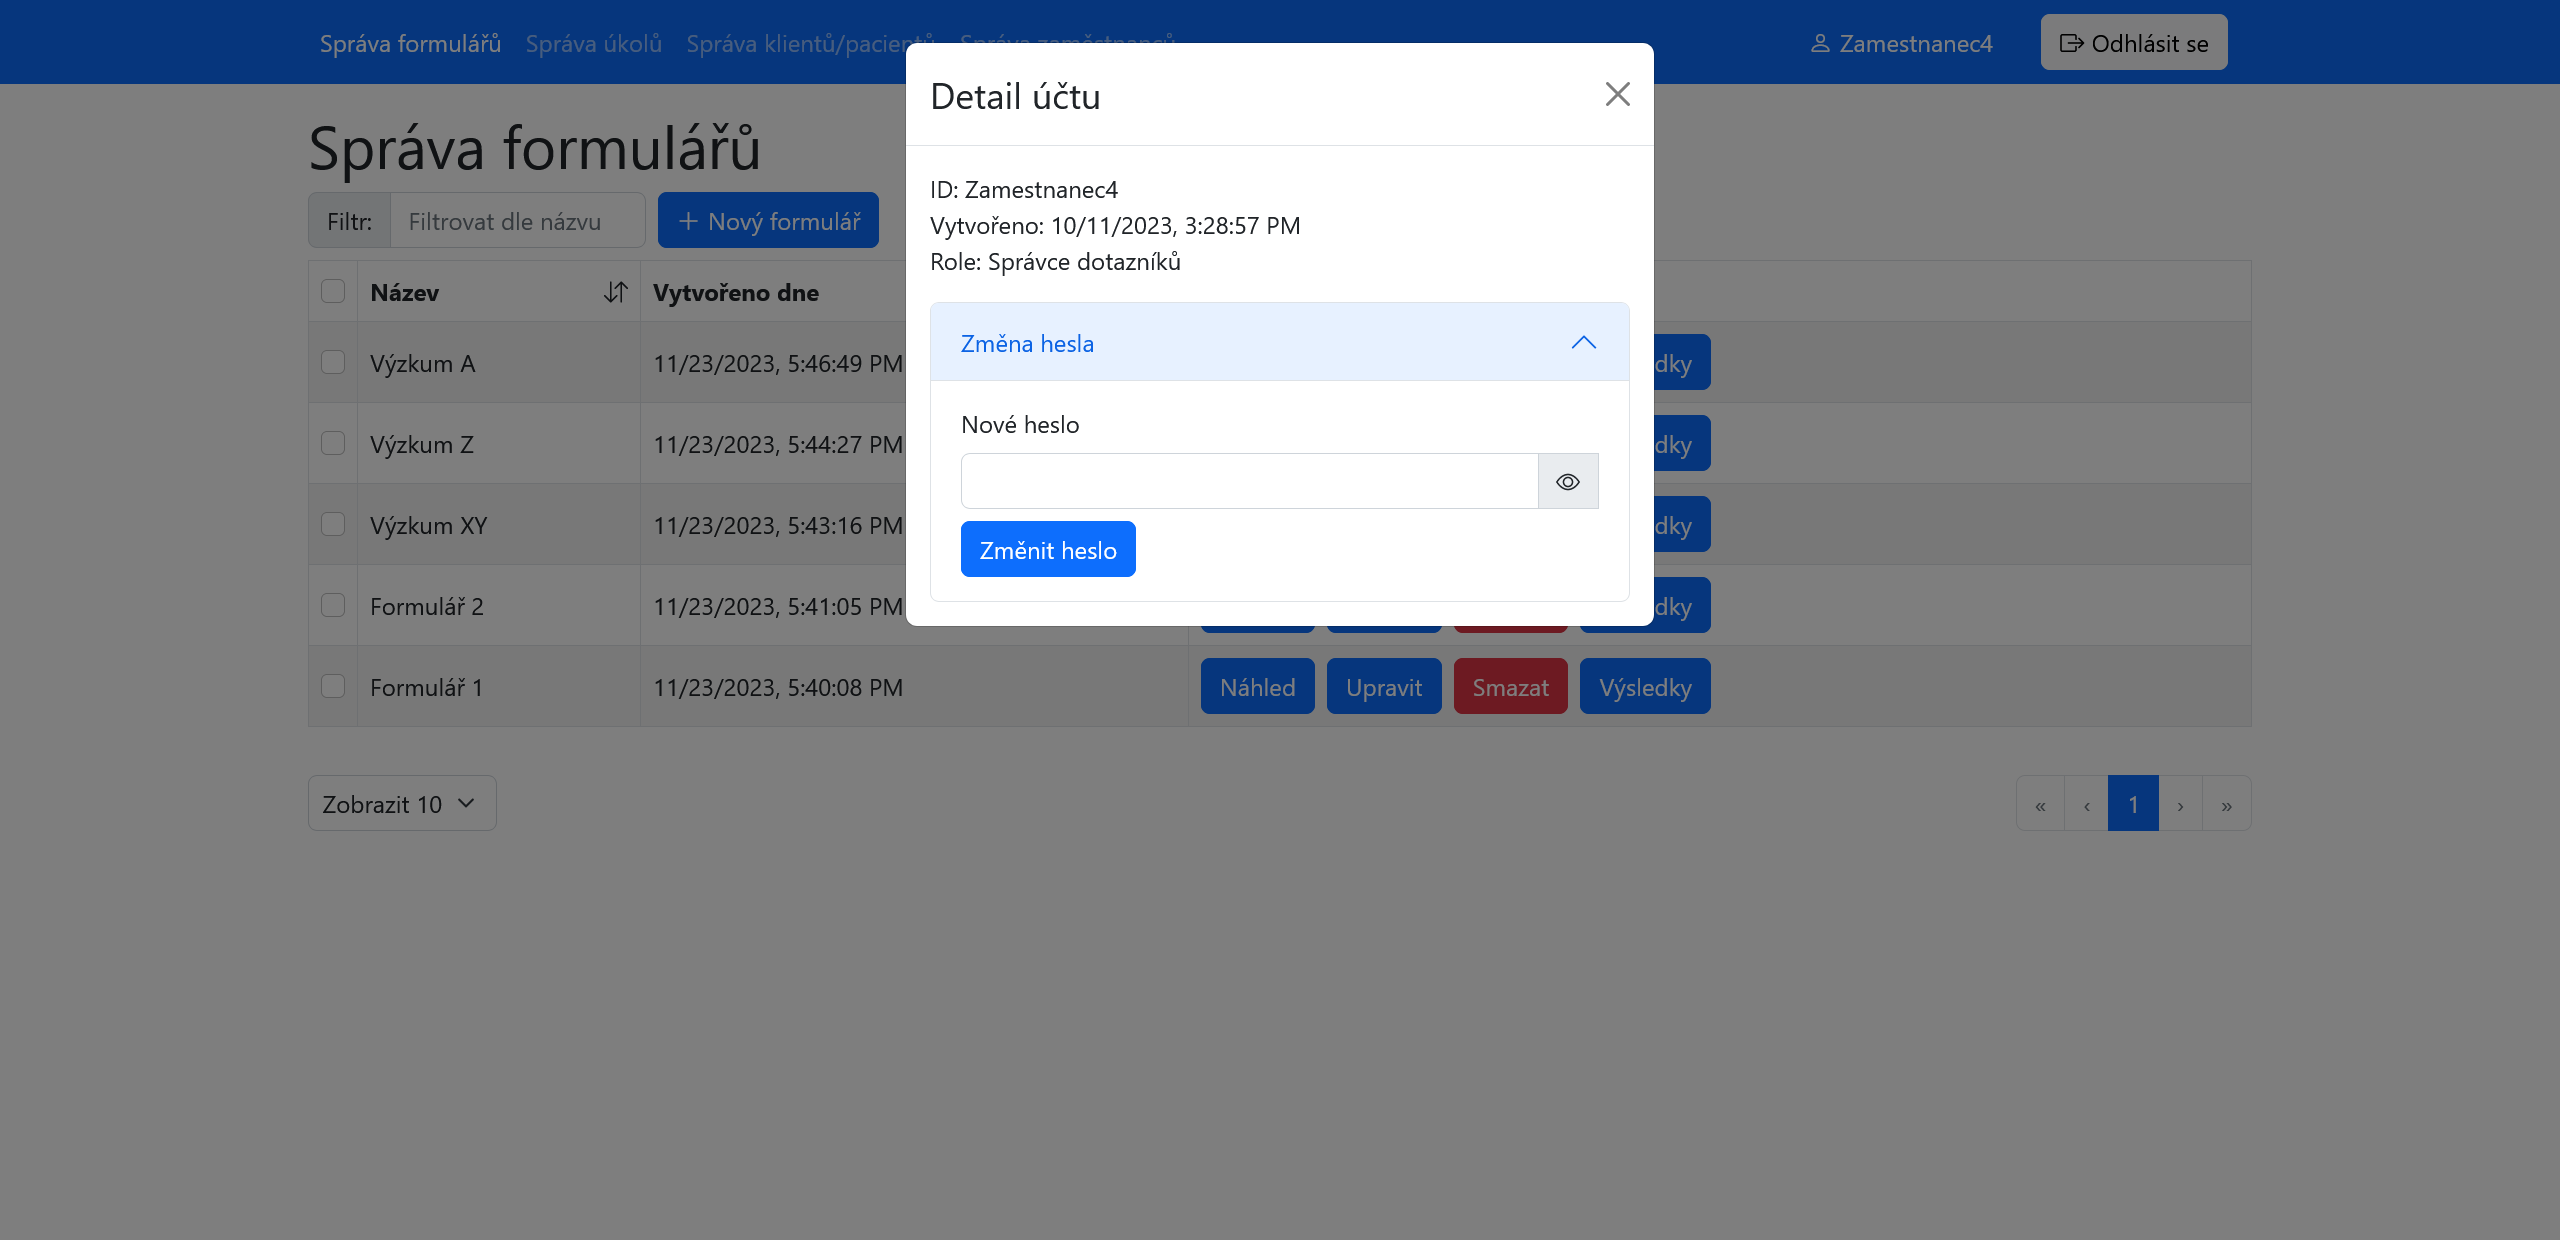
\includegraphics[width=\textwidth]{../img/screenshots/zmena-hesla-zamestnanec}
    \caption{Změna hesla vlastního účtu}\label{fig:zmena-hesla-zamestnanec}
\end{figure}


\section{Užívání aplikace z pohledu plnitele}\label{sec:uzivani-aplikace-z-pohledu-plnitele}

Nyní popišme proces z pohledu plnitele.
Jsou zde popsány veškeré funkce, které byly identifikovány jako požadavky na funkcionalitu dostupnou plniteli v kapitole o analýze požadavků~\ref{ch:analyza-pozadavku}.

Předpokládáme, že plnitel má již vytvořený účet a přihlásil se do aplikace, jak je popsáno v sekci~\ref{sec:prihlaseni}, která se věnuje přihlášení a tvorbě účtu.
Po přihlášení se plnitel dostane na přehled úkolů (Obr.~\ref{fig:prehled-ukolu-uzivatel-screenshot}).
Tato stránka zobrazuje všechny úkoly, které byly plniteli zadány.
Plnitel může úkol splnit stisknutím tlačítka \uv{Splnit}, čímž se dostane na stránku obsahující formulář k vyplnění (Obr.~\ref{fig:vyplneni-formulare-uzivatel-screenshot}).
Plnitel může v průběhu vyplňování formuláře stisknout tlačítko \uv{Uložit koncept}, čímž se formulář uloží do systému, ale neodešle se.
Při návratu na tuto stránku je uložený stav automaticky znovu načten.

\begin{figure}[H]
    \centering
    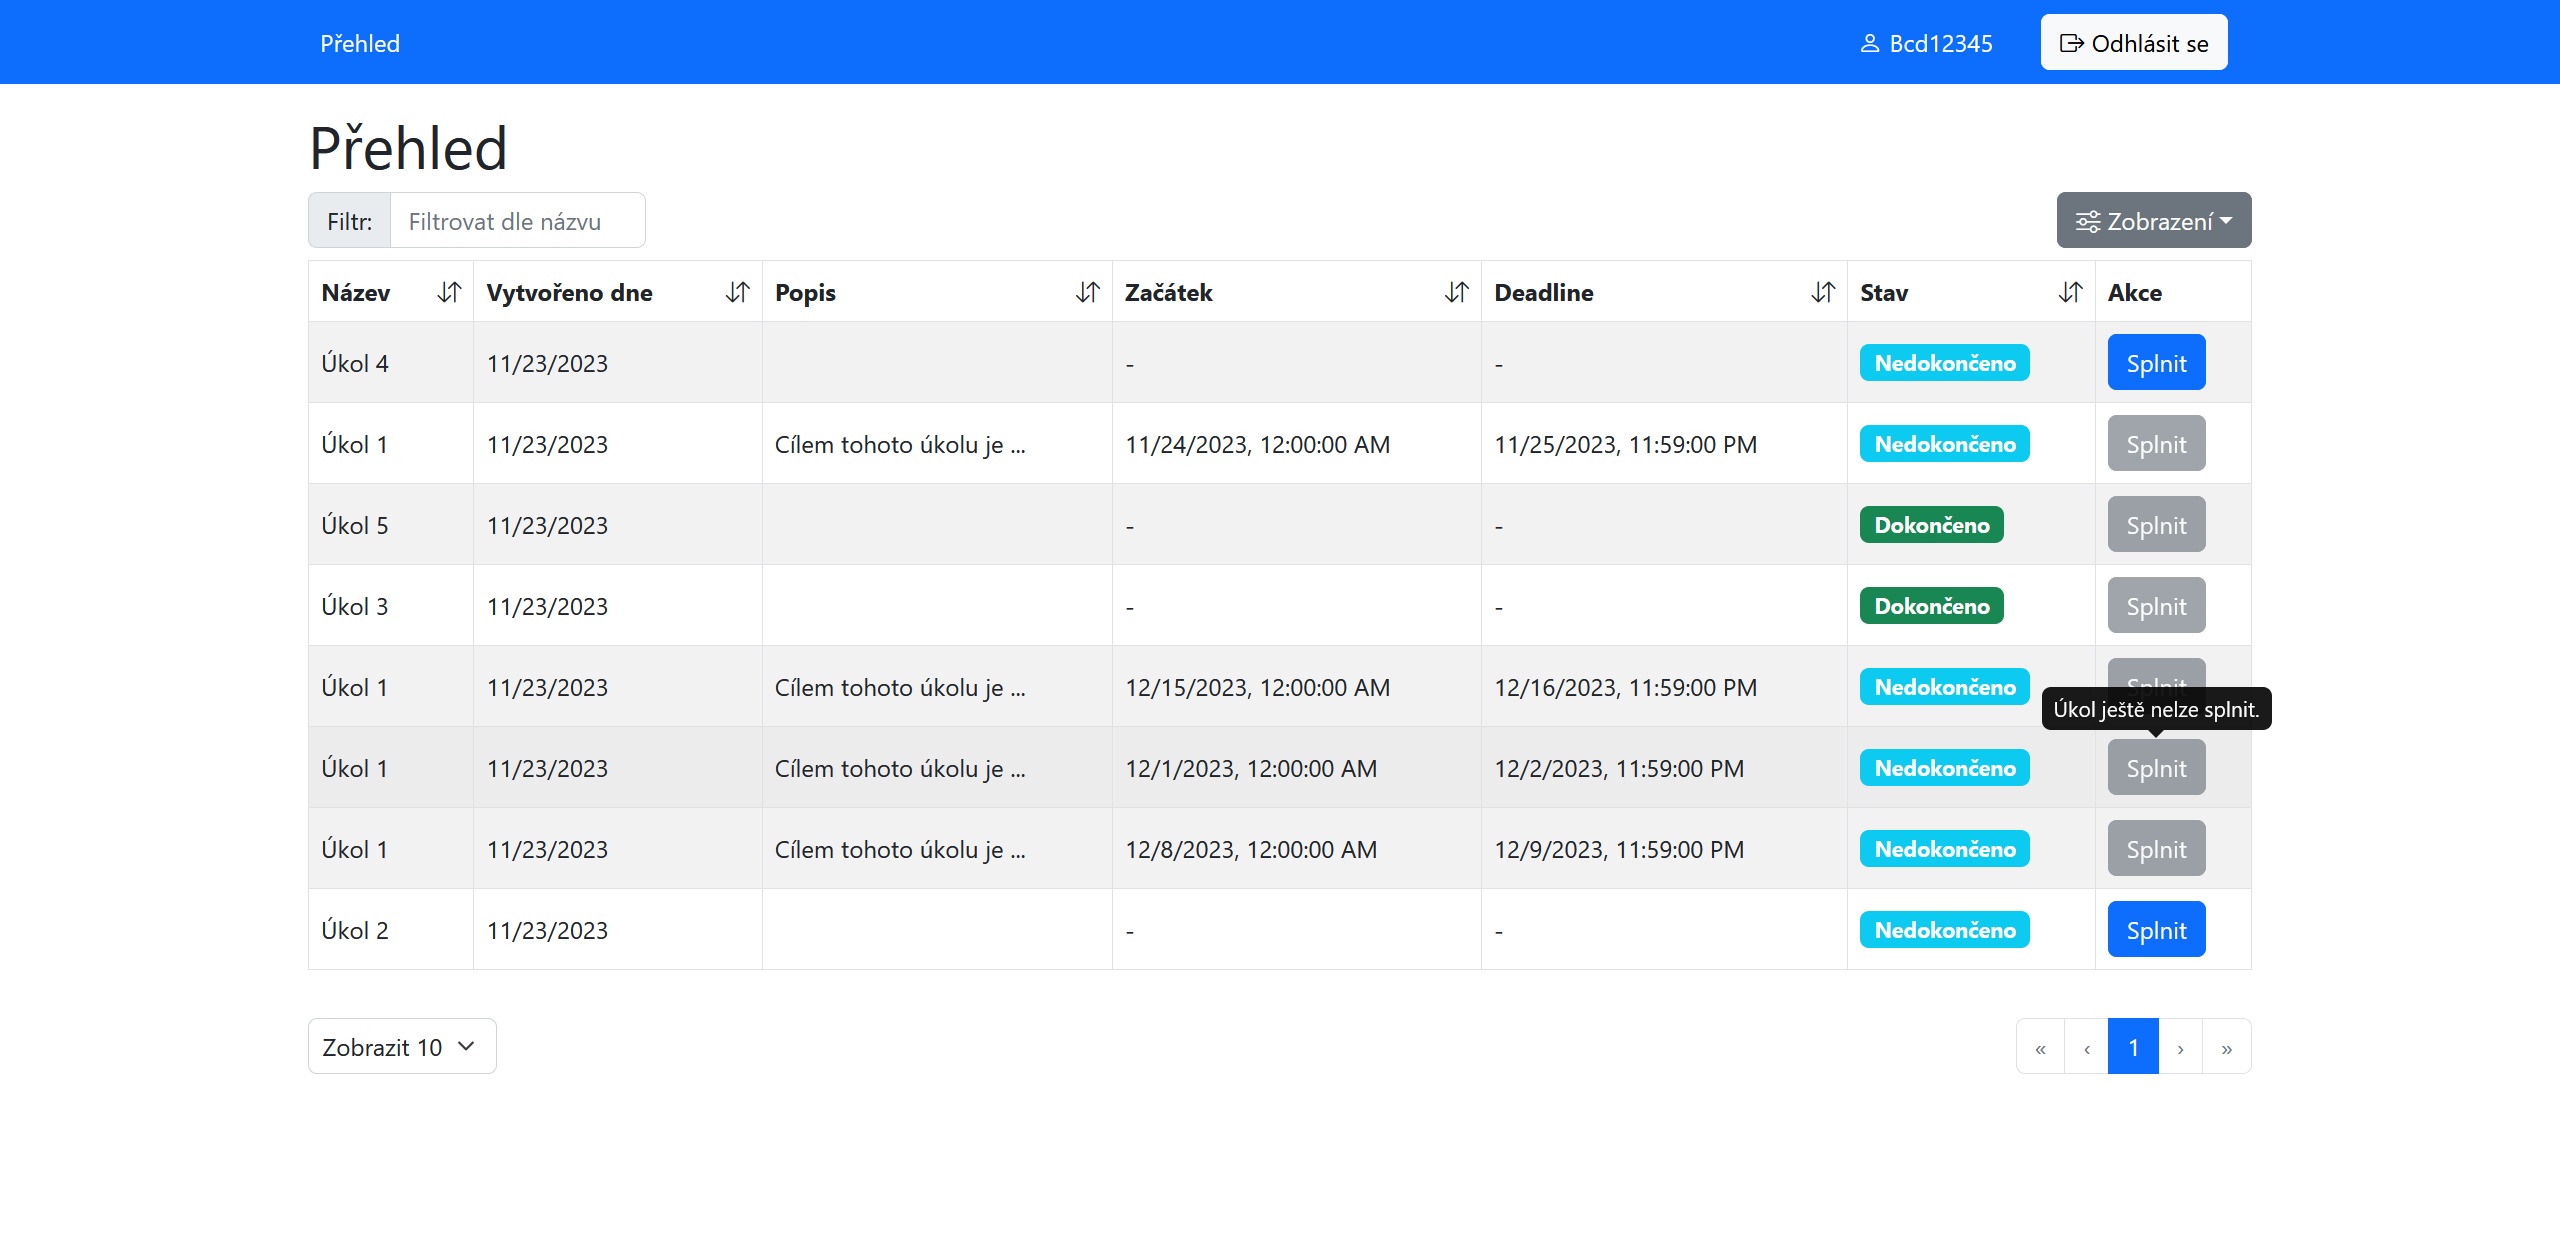
\includegraphics[width=\textwidth]{../img/screenshots/prehled-uzivatel}
    \caption{Přehled úkolů uživatele}\label{fig:prehled-ukolu-uzivatel-screenshot}
\end{figure}

\begin{figure}[H]
    \centering
    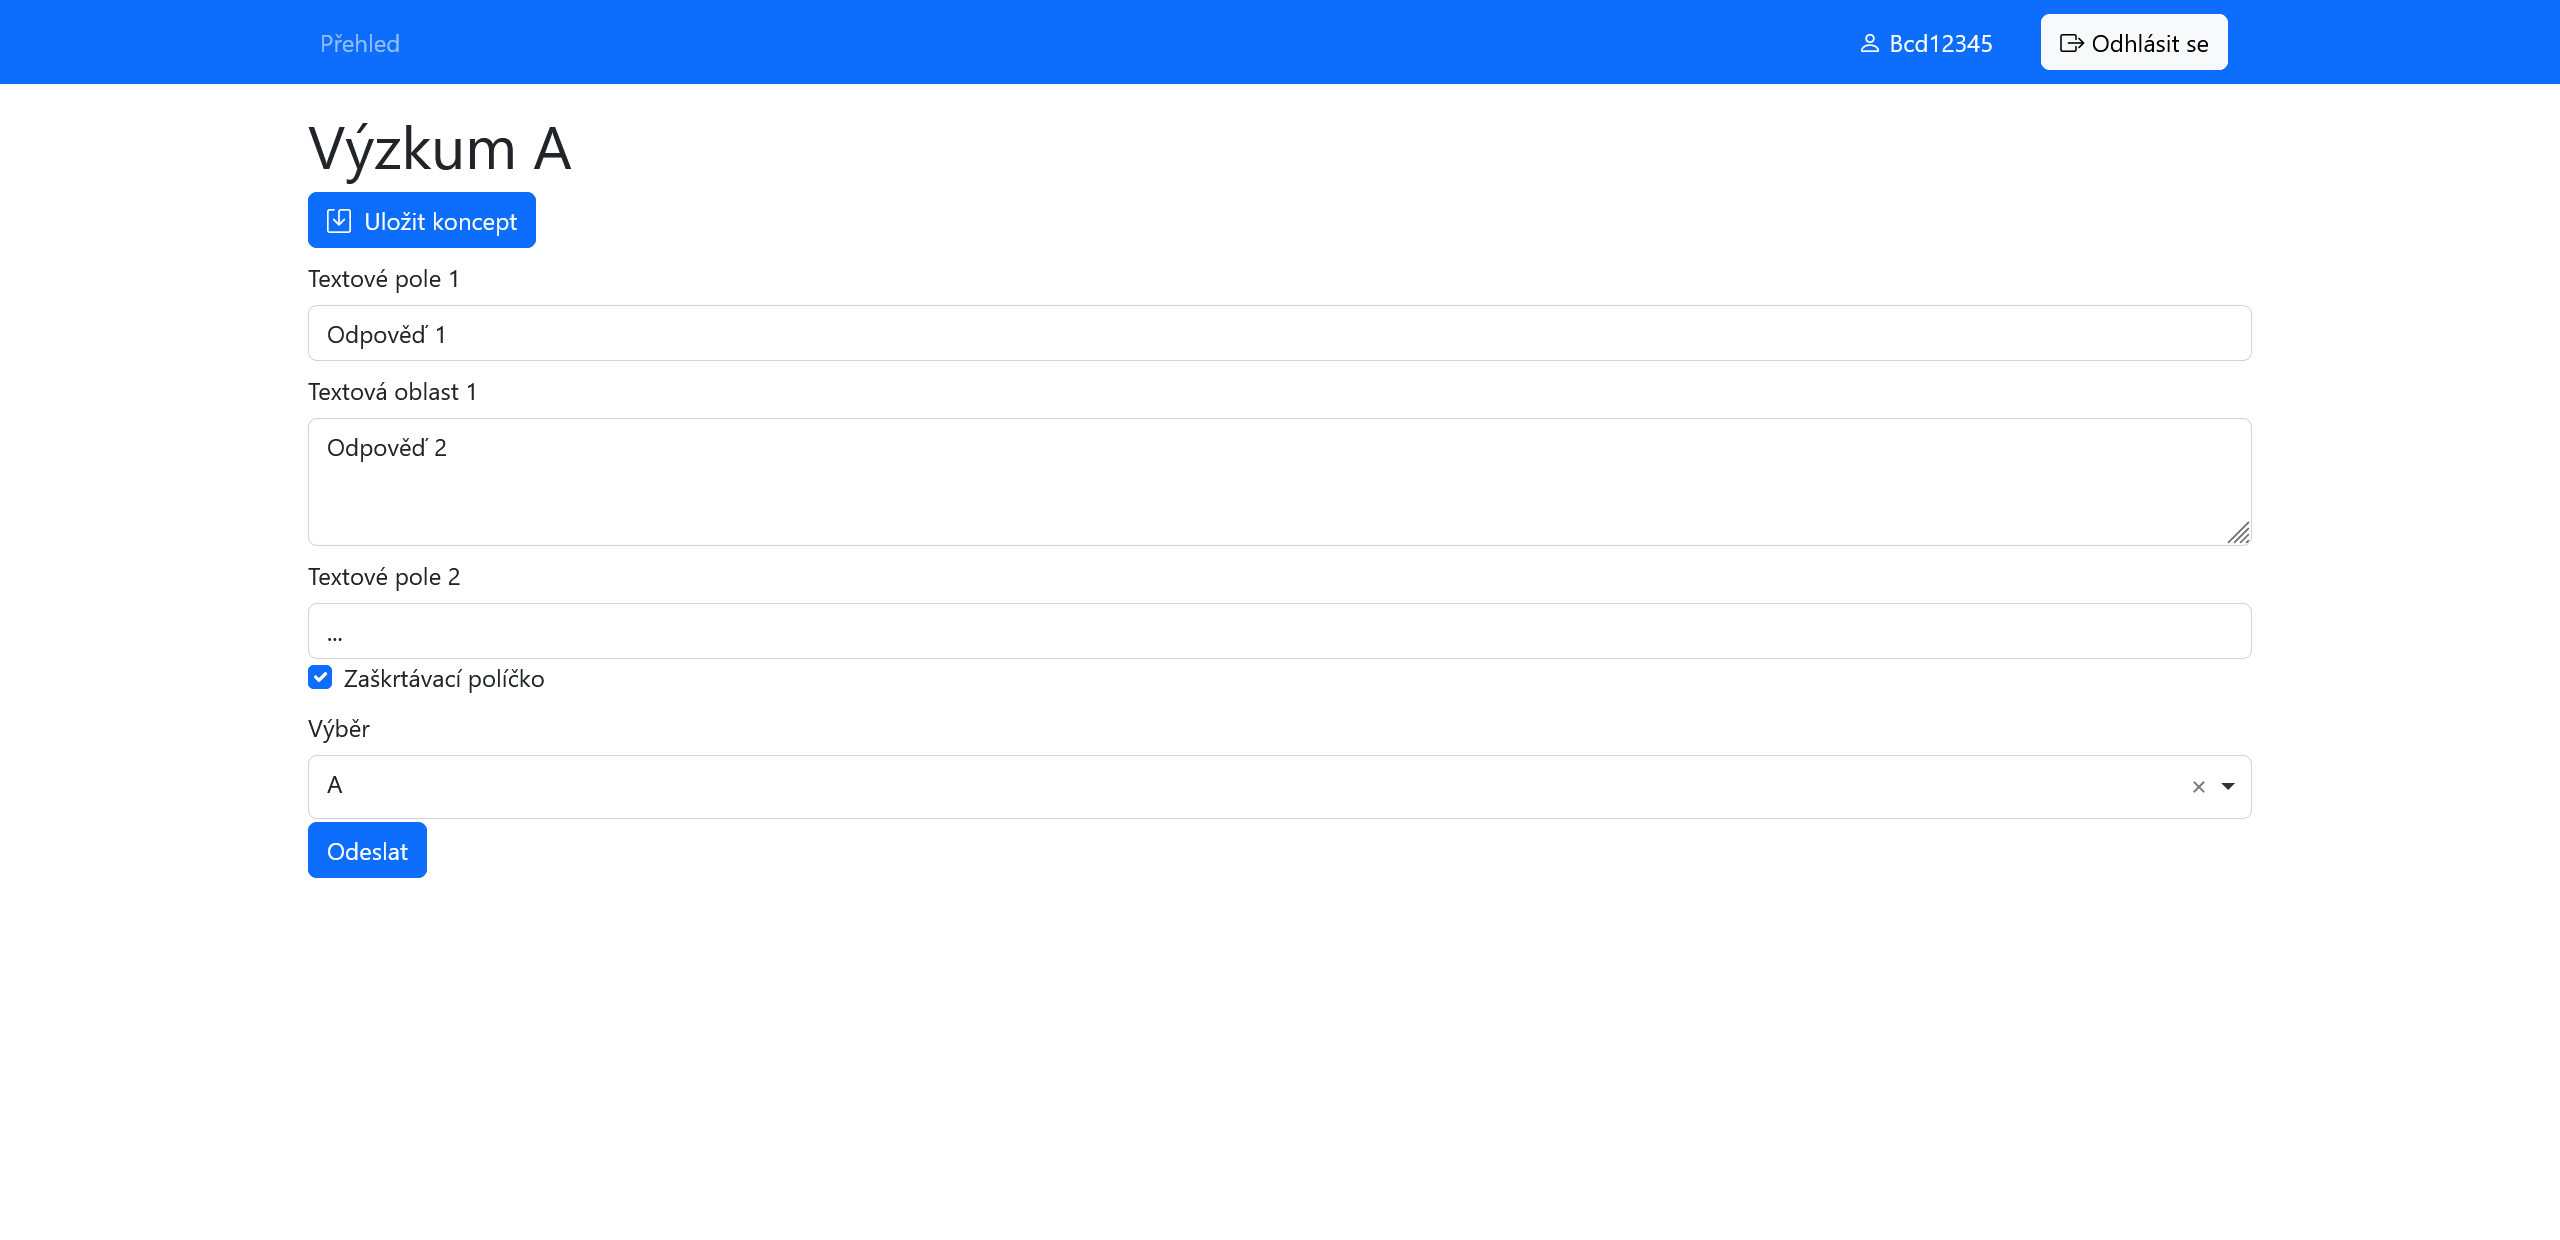
\includegraphics[width=\textwidth]{../img/screenshots/vyplneni-formulare-uzivatel}
    \caption{Vyplnění formuláře plnitelem}\label{fig:vyplneni-formulare-uzivatel-screenshot}
\end{figure}

Uživatel si může zobrazit detail svého účtu (Obr.~\ref{fig:zmena-hesla-uzivatel}) kliknutím na své ID v pravém horním rohu aplikace.
V okně detailu účtu může zaměstnanec změnit své heslo.
Pro změnu hesla je nutno zadat nové heslo a stisknout tlačítko \uv{Změnit heslo}.
Heslo musí obsahovat alespoň jedno velké písmeno, alespoň jedno malé písmeno a alespoň jedno číslo.
Pro manuální kontrolu hesla je možno zobrazit obsah hesla stisknutím tlačítka se symbolem oka.

\begin{figure}[H]
    \centering
    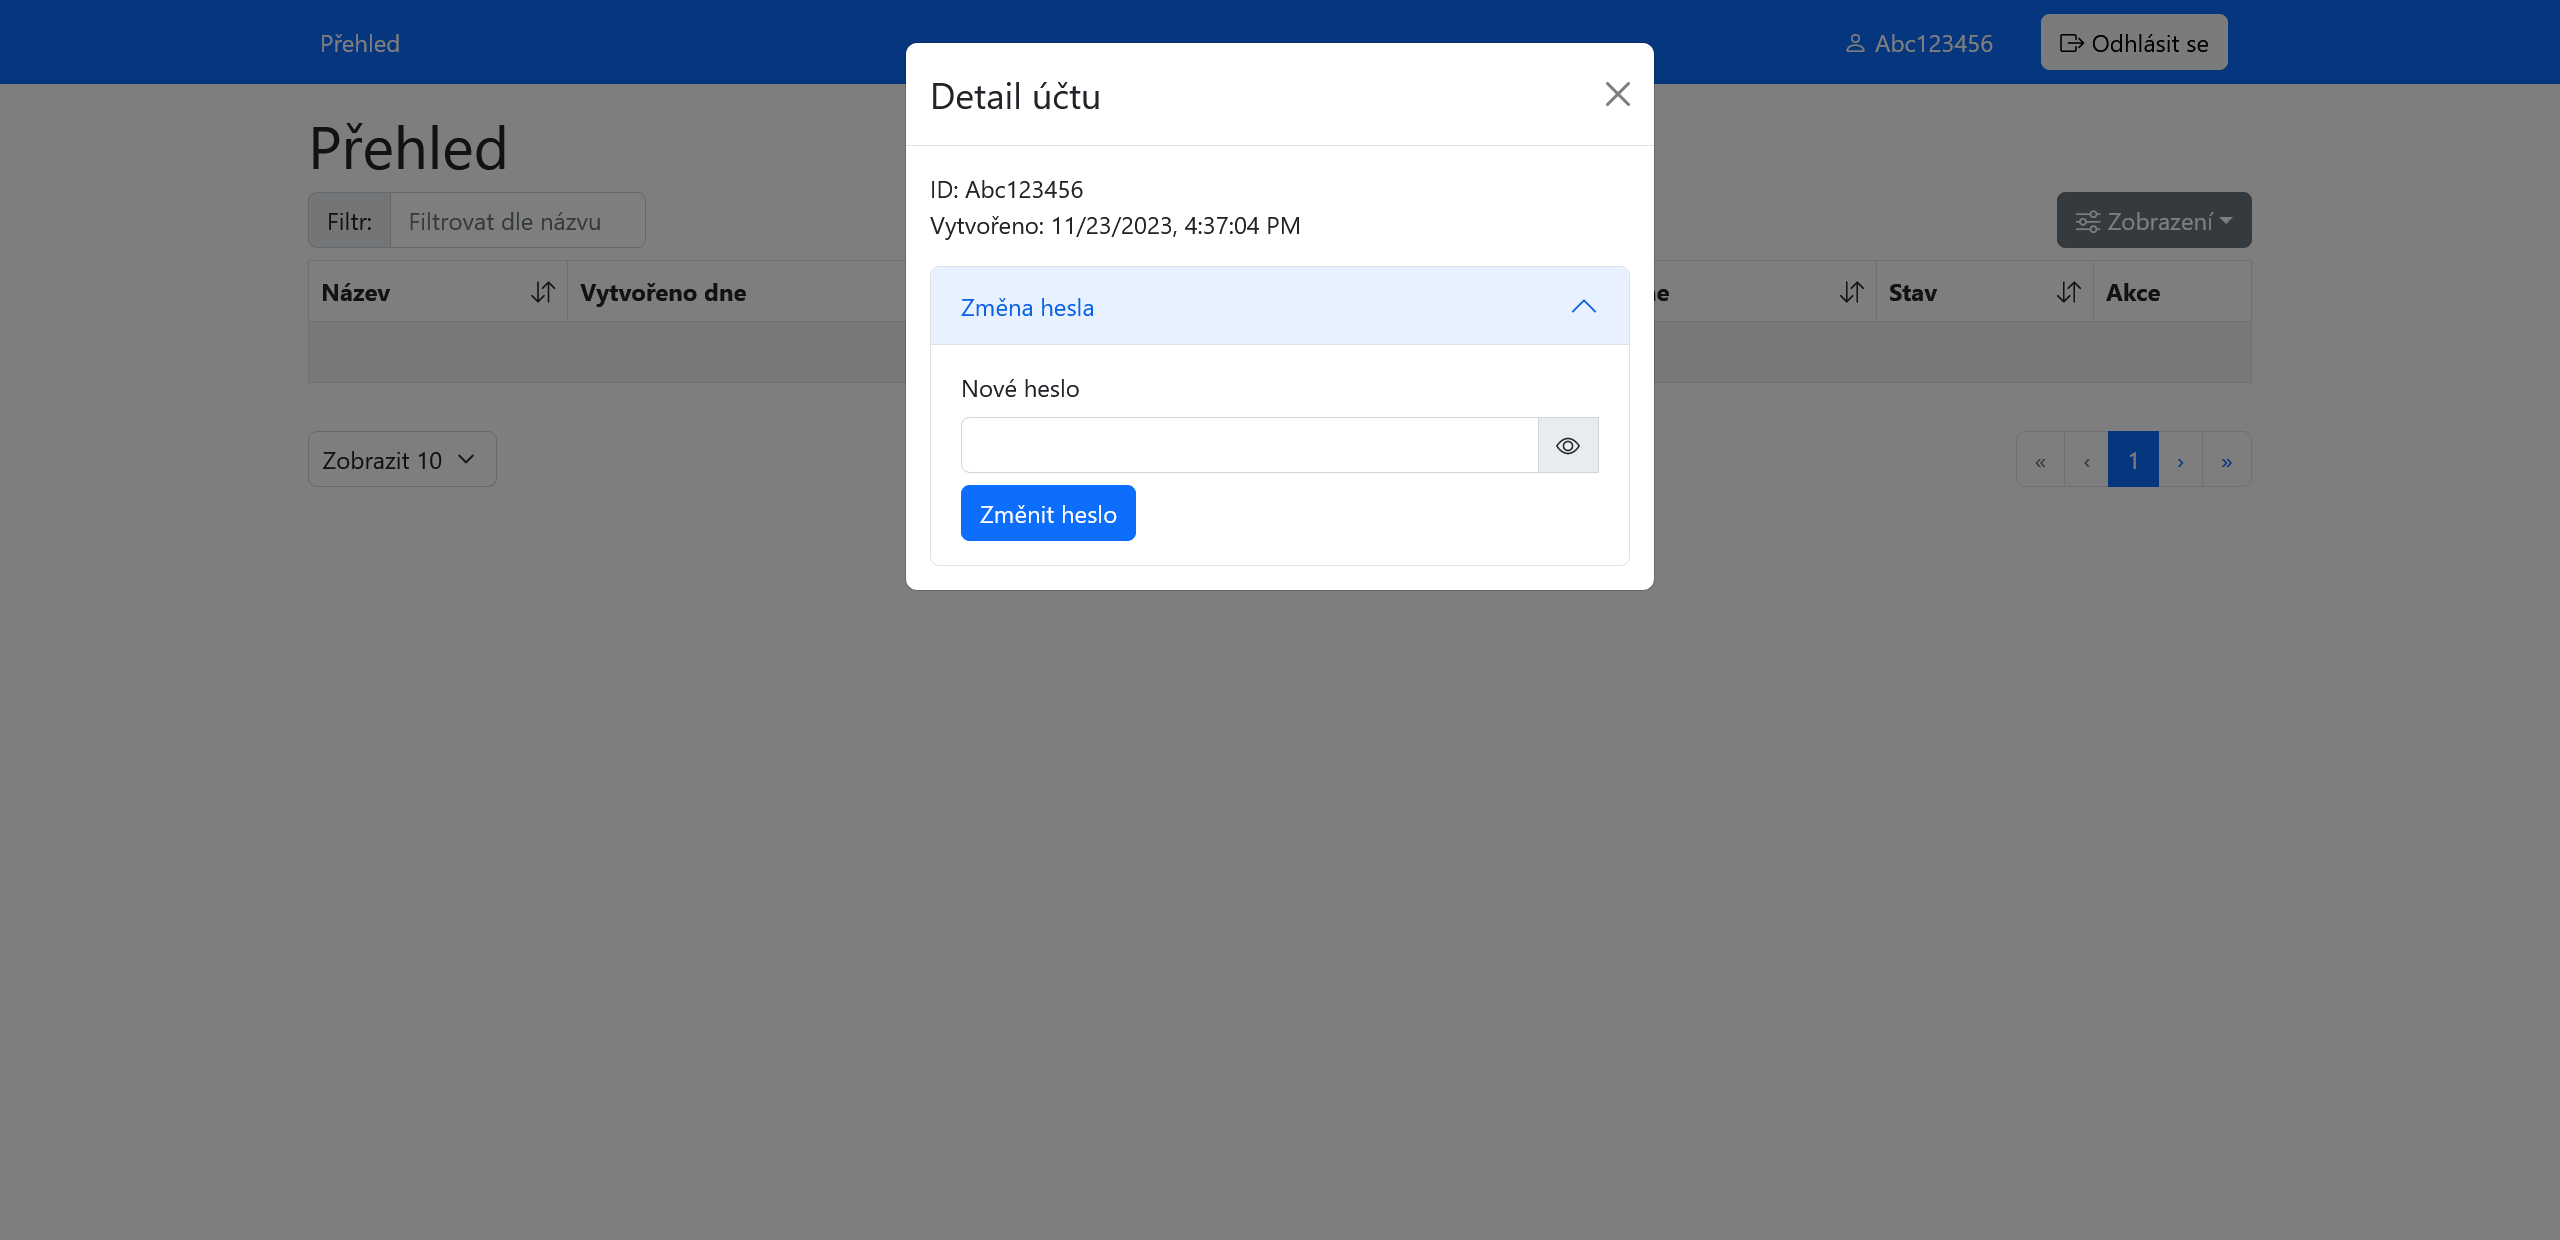
\includegraphics[width=\textwidth]{../img/screenshots/zmena-hesla-uzivatel}
    \caption{Změna hesla vlastního účtu}\label{fig:zmena-hesla-uzivatel}
\end{figure}

\chapter{Zhodnocení vývoje}\label{ch:zhodnoceni-vyvoje}

V této kapitole bych se chtěl ohlédnout zpátky, zhodnotit průběh celého vývoje a sepsat získané zkušenosti.


\section{Zhodnocení architektury}\label{sec:zhodnoceni-architektury}

Tento projekt byl vyvíjen jako distribuovaný systém.
Toto rozhodnutí pramenilo z mé nezkušenosti a zpětně ho považuji za chybné.
Distribuovaná architekura je vhodná pro specifické projekty, které dokáží těžit z výhod, které tato architektura poskytuje.
Tento projekt získal pouze minimum výhod, ale musel řešit všechnu komplexitu, která je s distribuovanými systémy spojena.


\section{Zkušenost s Form.io}\label{sec:zkusenost-s-formio}

Systém spravující formuláře Form.io na mě na začátku působil velmi profesionálně a vyspěle.
Narazil jsem však na mnoho problémů a nedostatků, které mi výrazně zkomplikovaly práci.
Software má mnoho dokumentace, ale některé části jsou nesrozumitelné a některé funkce jsou nedostatečně zdokumentované.
Klientské knihovny mají mj.\ špatnou podporu TypeScript, nepodporují všechny funkce serveru a mají špatně navržené rozhraní.
Po několika měsících práce jsem došel k závěru, že některé klientské knihovny je potřeba kompletně nahradit vlastním řešením.

Dalším problémem byla špatná spolupráce se správci projektu.
V průběhu mé práce jsem narazil na nedostatky software Form.io či dokumentace a tyto nedostatky jsem vždy nahlásil, či jsem je sám opravil.
Většina z nahlášených chyb dodnes nebyly adresovány a návrhy na mé vylepšení nebyly přijaty.

Kdybych tento projekt začínal znovu, mnohem více bych se snažil zadavateli rozmluvit požadavek na ukládání dat na vlastním serveru.
Tento požadavek je totiž hlavním důvodem, proč jsem se nakonec rozhodl pro použití Form.io.
Myslím si, že existuje mnoho lepších řešení pro správu formulářů, ale jedná se o cloudové služby.
V průběhu vývoje jsem se dozvěděl o \href{https://www.hhs.gov/hipaa/index.html}{HIPAA} certifikaci.
Software držící tuto certifikaci musí splňovat přísná pravidla pro ukládání zdravotnických dat.
Tuto certifikaci má mnoho z nástrojů zmiňovaných v kapitole~\ref{ch:analyza-existujicich-reseni-pro-praci-s-formulari}.
Myslím si, že užití nástroje s touto certifikací pro tvorbu a správu formulářů by byl nejlepší kompromis mezi bezpečností a kvalitou nástroje.
O této možnosti jsme však já ani zadavatel nevěděli a proto jsme se rozhodli pro použití Form.io.


\section{Zkušenost s NextJS}\label{sec:zkusenost-s-nextjs}

Rád bych také popsal svou zkušenost s framework NextJS\@.
Framework mi poskytl mnoho skvělých funkcí jako je routing, caching a také sdílení a zanořování layoutů.
Framework má skvělou dokumentaci a velkou aktivní komunitu.
Narazil jsem však i na několik problémů.

První problém byl s tzv. \textit{hot module replacement}.
Tato funkce umožňuje přidat, odebrat nebo vyměnit moduly za běhu aplikace bez nutnosti dalšího načtení celé stránky~\cite{hot-module-replacement-definition}.
Kompilační systém reaguje na změny souborů, které hlásí souborový systém, a následně aplikuje změny za běhu aplikace.
Pokud však vývojový server pustíme v Docker kontejneru, kde uděláme mount složky s kódem z hostitelského systému Windows, tak se změny v souborech nedetekují.
Tato chyba v \href{https://learn.microsoft.com/en-us/windows/wsl/about}{Windows subsystem for Linux (WSL)} je známá již od roku 2019 a zatím nebyla opravena (viz \href{https://github.com/microsoft/WSL/issues/4739}{diskuze v Github issue}).

Dalším problémem byla omezenost middleware, který NextJS poskytuje.
Middleware je kód, který je spuštěn před zpracováním všech požadavků na server.
Tento kód však běží v speciálním optimalizovaném prostředí nazývané \textit{\href{https://edge-runtime.vercel.app/}{edge runtime}}.
Edge runtime je velmi omezené prostředí a spoustu knihoven na něm nelze použít.
Důsledky toho jsou, že například nelze použít populární knihovny pro logování (\href{https://github.com/pinojs/pino}{Pino}, \href{https://github.com/winstonjs/winston}{Winston}, apod.) ani knihovnu \href{https://github.com/axios/axios}{axios}, která poskytuje alternativu k nativnímu fetch API\@.
NextJS v tuto chvíli nedovoluje použití jiného běhové prostředí pro middleware.

Posledním problémem byla implementace \textit{\href{https://developer.mozilla.org/en-US/docs/Web/HTTP/CSP}{content security policy}}.
Content security policy je bezpečnostní vrstva, která zabraňuje určitým typům útoků jako je například \href{https://developer.mozilla.org/en-US/docs/Glossary/Cross-site_scripting}{cross-site scripting (XSS)}.
Pro použití tohoto bezpečnostního prvku je potřeba nakonfigurovat hlavičky HTTP odpovědí a také modifikovat zdrojový kód stránky.
Podpora tohoto bezpečnostního mechanismu je v NextJS aktivně vyvíjena, ale v době psaní této práce nebyla plně funkční, což snižuje bezpečnost aplikace.


\section{Open-source vývoj}\label{sec:open-source-vyvoj}

Při vývoji jsem narazil na mnoho chyb a nedostatků v použitých nástrojích a knihovnách.
Tyto chyby jsem hlásil správcům jednotlivých projektů a některé jsem dokonce sám opravil.
V případě některých projektů byla komunikace se správci velmi dobrá a chyby byly rychle opraveny.
V některých případě jsem však narazil na rozdílnosti v názorech na správné řešení problémů nebo jsem se nedočkal žádné reakce.
Zde je výčet issues a pull requestů, které jsem vytvořil:

\begin{itemize}
    \item
    \href{https://github.com/formio/react/issues/522}{Chyba v internacionalizaci komponenty poskytované knihovnou}
    \item
    \href{https://github.com/formio/react/pull/538}{Oprava chyby v internacionalizaci komponenty poskytované knihovnou}
    \item
    \href{https://github.com/formio/formio-app-formio/issues/35}{Bezpečnostní chyba v Form.io klientské aplikace}
    \item
    \href{https://github.com/formio/formio/issues/1555}{Chybějící dokumentace API endpointu}
    \item
    \href{https://github.com/formio/formio/issues/1485}{Chyba ve verzi databáze}
    \item
    \href{https://github.com/formio/formio-app-formio/issues/34}{Návrh na zlepšení organizace repozitáře}
    \item
    \href{https://github.com/formio/react/issues/523}{Použití zastaralého API}
    \item
    \href{https://github.com/tgreyuk/typedoc-plugin-markdown/issues/429}{Chyba v pluginu do Docusaurus}
    \item
    \href{https://github.com/tgreyuk/typedoc-plugin-markdown/issues/440}{Návrh na vylepšení pluginu do Docusaurus}
    \item
    \href{https://github.com/react-bootstrap/react-bootstrap/issues/6671}{Nefunkční příklad v dokumentaci}
    \item
    \href{https://github.com/gajus/eslint-plugin-jsdoc/issues/1138}{Návrh na vylepšení chování statické analýzy kódu}
    \item
    \href{https://github.com/MrFlynn/upload-to-netlify-action/issues/17}{Chyba v dokumentaci GitHub Action pro upload na Netlify}
\end{itemize}


\section{Spolupráce s NUDZ}\label{sec:spoluprace-s-nudz}

Spolupráce s Národním ústavem duševního zdraví nebyla vždy jednoduchá.
Nízká technická znalost zaměstnanců byla větší problém než jsem očekával.
V některých chvílích jsem nedokázal klást ty správné otázky a nepodařilo se mi zachytit všechny důležité informace o doméně.
Celá spolupráce byla značně ztížena tím, že se v průběhu vývoje několikrát změnila osoba, která se mnou spolupracovala a komunikovala.
Celkově jsem však spokojený s výsledkem a věřím, že aplikace bude využívána a pomůže zlepšit kvalitu poskytované péče.

\chapter*{Závěr}
\addcontentsline{toc}{chapter}{Závěr}

Na závěr bych se chtěl ohlédnout zpátky a zhodnotit průběh celého vývoje.


\section{Zhodnocení architektury}\label{sec:zhodnoceni-architektury}

Tento projekt byl vyvíjen jako distribuovaný systém.
Toto rozhodnutí pramenilo z mé nezkušenosti a zpětně ho považuji za chybné.
Distribuovaná architekura je vhodná pro vyspělé projekty, které dokáží těžit z výhod, které tato architektura poskytuje.
Tento projekt získal pouze minimum výhod, ale musel řešit všechnu komplexitu, která je s distribuovanými systémy spojena.
Dospěl jsem k názoru, že systém by měl být vyvíjen jako distribuovaný pouze a jen v případě, že je to nezbytně nutné.


\section{Zhodnocení výběru technologií}\label{sec:vyber-technologii-zaver}

V této sekci bych chtěl zhodnotit výběr technologií, které jsem použil při vývoji aplikace.
Hodnocení se bude týkat pouze technologií, které měly výrazný vliv na vývoj aplikace.

\subsection{Zkušenost s Form.io}\label{subsec:zkusenost-s-formio}

Systém spravující formuláře Form.io na mě na začátku působil velmi profesionálně a vyspěle.
Narazil jsem však na mnoho problémů a nedostatků, které mi výrazně zkomplikovaly práci.
Software má mnoho dokumentace, ale některé části jsou nesrozumitelné a některé funkce jsou nedostatečně zdokumentované.
Klientské knihovny mají mj.\ špatnou podporu TypeScript, nepodporují všechny funkce serveru a mají špatně navržené rozhraní.
Po několika měsících práce jsem došel k závěru, že některé klientské knihovny je potřeba kompletně nahradit vlastním řešením.

Dalším problémem byla špatná spolupráce se správci projektu.
V průběhu mé práce jsem narazil na nedostatky software Form.io či dokumentace a tyto nedostatky jsem vždy nahlásil, či jsem je dokonce sám opravil.
Většina z nahlášených chyb dodnes nebyly adresovány a návrhy na mé vylepšení nebyly přijaty.

Kdybych tento projekt začínal znovu, mnohem více bych se snažil zadavateli rozmluvit požadavek na ukládání dat na vlastním serveru.
Tento požadavek je totiž hlavním důvodem, proč jsem se nakonec rozhodl pro použití Form.io.
Myslím si, že existuje mnoho lepších řešení pro správu formulářů, ale jedná se o cloudové služby.
V průběhu vývoje jsem se dozvěděl o \href{https://www.hhs.gov/hipaa/index.html}{HIPAA} certifikaci.
Software držící tuto certifikaci musí splňovat přísná pravidla pro ukládání zdravotnických dat.
Tuto certifikaci má mnoho z nástrojů zmiňovaných v kapitole~\ref{ch:analyza-existujicich-reseni-pro-praci-s-formulari}.
Myslím si, že užití nástroje s touto certifikací pro tvorbu a správu formulářů by byl nejlepší kompromis mezi bezpečností a kvalitou nástroje.
O této možnosti jsme však já ani zadavatel nevěděli a proto jsme se rozhodli pro použití Form.io.

\subsection{Zkušenost s NextJS}\label{subsec:zkusenost-s-nextjs}

Rád bych také popsal svou zkušenost s framework NextJS\@.
Framework mi poskytl mnoho skvělých funkcí jako je routing, caching a také sdílení a zanořování layoutů.
Framework má skvělou dokumentaci a velkou aktivní komunitu.
Narazil jsem však i na několik problémů.

První problém byl s tzv. \textit{hot module replacement}.
Tato funkce umožňuje přidat, odebrat nebo vyměnit moduly za běhu aplikace bez nutnosti dalšího načtení celé stránky (\href{https://webpack.js.org/concepts/hot-module-replacement/}{zdroj}).
Kompilační systém reaguje na změny souborů, které hlásí souborový systém, a následně aplikuje změny za běhu aplikace.
Pokud však vývojový server pustíme v Docker kontejneru, kde uděláme mount složky s kódem z hostitelského systému Windows, tak se změny v souborech nedetekují.
Tato chyba v \href{https://learn.microsoft.com/en-us/windows/wsl/about}{Windows subsystem for Linux (WSL)} je známá již od roku 2019 a zatím nebyla opravena (viz \href{https://github.com/microsoft/WSL/issues/4739}{diskuze v Github issue}).

Dalším problémem byla omezenost middleware, který NextJS poskytuje.
Middleware je kód, který je spuštěn před zpracováním všech požadavků na server.
Tento kód však běží v speciálním optimalizovaném prostředí nazývané \textit{\href{https://edge-runtime.vercel.app/}{edge runtime}}.
Edge runtime je velmi omezené prostředí a spoustu knihoven na něm nelze použít.
Důsledky toho jsou, že například nelze použít populární knihovny pro logování (\href{https://github.com/pinojs/pino}{Pino}, \href{https://github.com/winstonjs/winston}{Winston}, apod.) ani knihovnu \href{https://github.com/axios/axios}{axios}, která poskytuje alternativu k nativnímu fetch API\@.
NextJS v tuto chvíli nedovoluje použití jiného běhové prostředí pro middleware.

Posledním problémem byla implementace \textit{\href{https://developer.mozilla.org/en-US/docs/Web/HTTP/CSP}{content security policy}}.
Content security policy je bezpečnostní vrstva, která zabraňuje určitým typům útoků jako je například \href{https://developer.mozilla.org/en-US/docs/Glossary/Cross-site_scripting}{cross-site scripting (XSS)}.
Pro použití tohoto bezpečnostního prvku je potřeba nakonfigurovat hlavičky HTTP odpovědí a také modifikovat zdrojový kód stránky.
Podpora tohoto bezpečnostního mechanismu je v NextJS aktivně vyvíjena, ale v době psaní této práce nebyla plně funkční, což snižuje bezpečnost aplikace.


\section{Zhodnocení testování aplikace}\label{sec:zhodnoceni-testovani-aplikace}

Serverová část aplikace je testována pomocí unit testů.
Testujeme pouze veřejné rozhraní všech modulů.
Objekt fungující jako proxy databáze byl nahrazen mock objekty.
V testech kontrolujeme, zda-li se volají konkrétní metody na mock objektech s očekávanými parametry.
Toto je doporučený přístup object-relational mapping knihovny Prisma, který je popsán v \href{https://www.prisma.io/docs/guides/testing/unit-testing}{dokumentaci}.
Tento přístup se mi vůbec neosvědčil.
Kontrola volání konkrétních metod vytváří obrovskou závislost na vnitřní implementaci testovaných metod.
Testy jsou velmi těžko udržovatelné a navíc poměrně dlouhé a složité.
Kdybych začínal znovu, tak bych se snažil primárně testovat privátní metody, které obsahují veškerou logiku mimo databázové operace.
Přestože tento způsob je také silně závislý na vnitřní implementaci testovaného modulu, tak je udržitelnější a jednodušší na implementaci.
Pro testování metod obsahující databázové operace bych zvážil použití in-memory databáze\footnote{In-memory databáze je databáze spoléhající primárně na vnitřní paměť pro ukládání dat (\href{https://aws.amazon.com/nosql/in-memory/}{zdroj})}.

\section{Open-source vývoj}\label{sec:open-source-vyvoj}

Při vývoji jsem narazil na mnoho chyb a nedostatků v použitých nástrojích a knihovnách.
Tyto chyby jsem hlásil správcům jednotlivých projektů a některé jsem dokonce sám opravil.
V případě některých projektů byla komunikace se správci velmi dobrá a chyby byly rychle opraveny.
V některých případě jsem však narazil na rozdílnosti v názorech na správné řešení problémů nebo jsem se nedočkal žádné reakce.
Zde je výčet issues a pull requestů, které jsem vytvořil:

\begin{itemize}
    \item
    \href{https://github.com/formio/react/issues/522}{Chyba v internacionalizaci komponenty poskytované knihovnou}
    \item
    \href{https://github.com/formio/react/pull/538}{Oprava chyby v internacionalizaci komponenty poskytované knihovnou}
    \item
    \href{https://github.com/formio/formio-app-formio/issues/35}{Bezpečnostní chyba v Form.io klientské aplikace}
    \item
    \href{https://github.com/formio/formio/issues/1555}{Chybějící dokumentace API endpointu}
    \item
    \href{https://github.com/formio/formio/issues/1485}{Chyba ve verzi databáze}
    \item
    \href{https://github.com/formio/formio-app-formio/issues/34}{Návrh na zlepšení organizace repozitáře}
    \item
    \href{https://github.com/formio/react/issues/523}{Použití zastaralého API}
    \item
    \href{https://github.com/tgreyuk/typedoc-plugin-markdown/issues/429}{Chyba v pluginu do Docusaurus}
    \item
    \href{https://github.com/tgreyuk/typedoc-plugin-markdown/issues/440}{Návrh na vylepšení pluginu do Docusaurus}
    \item
    \href{https://github.com/react-bootstrap/react-bootstrap/issues/6671}{Nefunkční příklad v dokumentaci}
    \item
    \href{https://github.com/gajus/eslint-plugin-jsdoc/issues/1138}{Návrh na vylepšení chování statické analýzy kódu}
    \item
    \href{https://github.com/MrFlynn/upload-to-netlify-action/issues/17}{Chyba v dokumentaci GitHub Action pro upload na Netlify}
\end{itemize}


\section{Spolupráce s NUDZ}\label{sec:spoluprace-s-nudz}

Spolupráce s Národním ústavem duševního zdraví nebyla vždy jednoduchá.
Nízká technická znalost zaměstnanců byla větší problém než jsem očekával.
V některých chvílích jsem nedokázal klást ty správné otázky a nepodařilo se mi zachytit všechny důležité informace o doméně.
Celá spolupráce byla značně ztížena tím, že se v průběhu vývoje několikrát změnila osoba, která se mnou spolupracovala a komunikovala.
Celkově jsem však spokojený s výsledkem a věřím, že aplikace bude využívána a pomůže zlepšit kvalitu poskytované péče.

\section{Shrnutí}\label{sec:shrnuti}

V této práci jsme se zabývali vývojem webové aplikace pro monitorování mentálního zdraví.
Na začátku jsme detailně analyzovali požadavky zadavatele a vytvořili návrh aplikace.
Poté jsme rozebrali proces vývoje, popsali technické detaily a sepsali uživatelskou dokumentaci.
Na závěr jsme zhodnotili průběh celého vývoje a výslednou aplikaci.

%%% Seznam použité literatury
%%% Seznam použité literatury (bibliografie)
%%%
%%% Pro vytváření bibliografie používáme bibTeX. Ten zpracovává
%%% citace v textu (např. makro \cite{...}) a vyhledává k nim literaturu
%%% v souboru literatura.bib.
%%%
%%% Příkaz \bibliographystyle určuje, jakým stylem budou citovány odkazy
%%% v textu. V závorce je název zvoleného souboru .bst. Styly plainnat
%%% a unsrt jsou standardní součástí latexových distribucí. Styl czplainnat
%%% je dodáván s touto šablonou a bibTeX ho hledá v aktuálním adresáři.

\bibliographystyle{czplainnat}    %% Autor (rok) s českými spojkami
% \bibliographystyle{plainnat}    %% Autor (rok) s anglickými spojkami
% \bibliographystyle{unsrt}       %% [číslo]

\renewcommand{\bibname}{Seznam použité literatury}

%%% Vytvoření seznamu literatury. Pozor, pokud jste necitovali ani jednu
%%% položku, seznam se automaticky vynechá.

\bibliography{literatura}

%%% Kdybyste chtěli bibliografii vytvářet ručně (bez bibTeXu), lze to udělat
%%% následovně. V takovém případě se řiďte normou ISO 690 a zvyklostmi v oboru.

% \begin{thebibliography}{99}
%
% \bibitem{lamport94}
%   {\sc Lamport,} Leslie.
%   \emph{\LaTeX: A Document Preparation System}.
%   2. vydání.
%   Massachusetts: Addison Wesley, 1994.
%   ISBN 0-201-52983-1.
%
% \end{thebibliography}


%%% Obrázky v bakalářské práci
%%% (pokud jich je malé množství, obvykle není třeba seznam uvádět)
\listoffigures

%%% Tabulky v bakalářské práci (opět nemusí být nutné uvádět)
%%% U matematických prací může být lepší přemístit seznam tabulek na začátek práce.
%\listoftables

%%% Použité zkratky v bakalářské práci (opět nemusí být nutné uvádět)
%%% U matematických prací může být lepší přemístit seznam zkratek na začátek práce.
%\chapwithtoc{Seznam použitých zkratek}

%%% Přílohy k bakalářské práci, existují-li. Každá příloha musí být alespoň jednou
%%% odkazována z vlastního textu práce. Přílohy se číslují.
%%%
%%% Do tištěné verze se spíše hodí přílohy, které lze číst a prohlížet (dodatečné
%%% tabulky a grafy, různé textové doplňky, ukázky výstupů z počítačových programů,
%%% apod.). Do elektronické verze se hodí přílohy, které budou spíše používány
%%% v elektronické podobě než čteny (zdrojové kódy programů, datové soubory,
%%% interaktivní grafy apod.). Elektronické přílohy se nahrávají do SISu a lze
%%% je také do práce vložit na CD/DVD. Povolené formáty souborů specifikuje
%%% opatření rektora č. 72/2017.
\appendix


\chapter{Přílohy}\label{ch:prilohy}


\section{Vstupy pro analýzu požadavků}\label{sec:analyza-pozadavku-prilohy}

\begin{figure}[H]
    \centering
    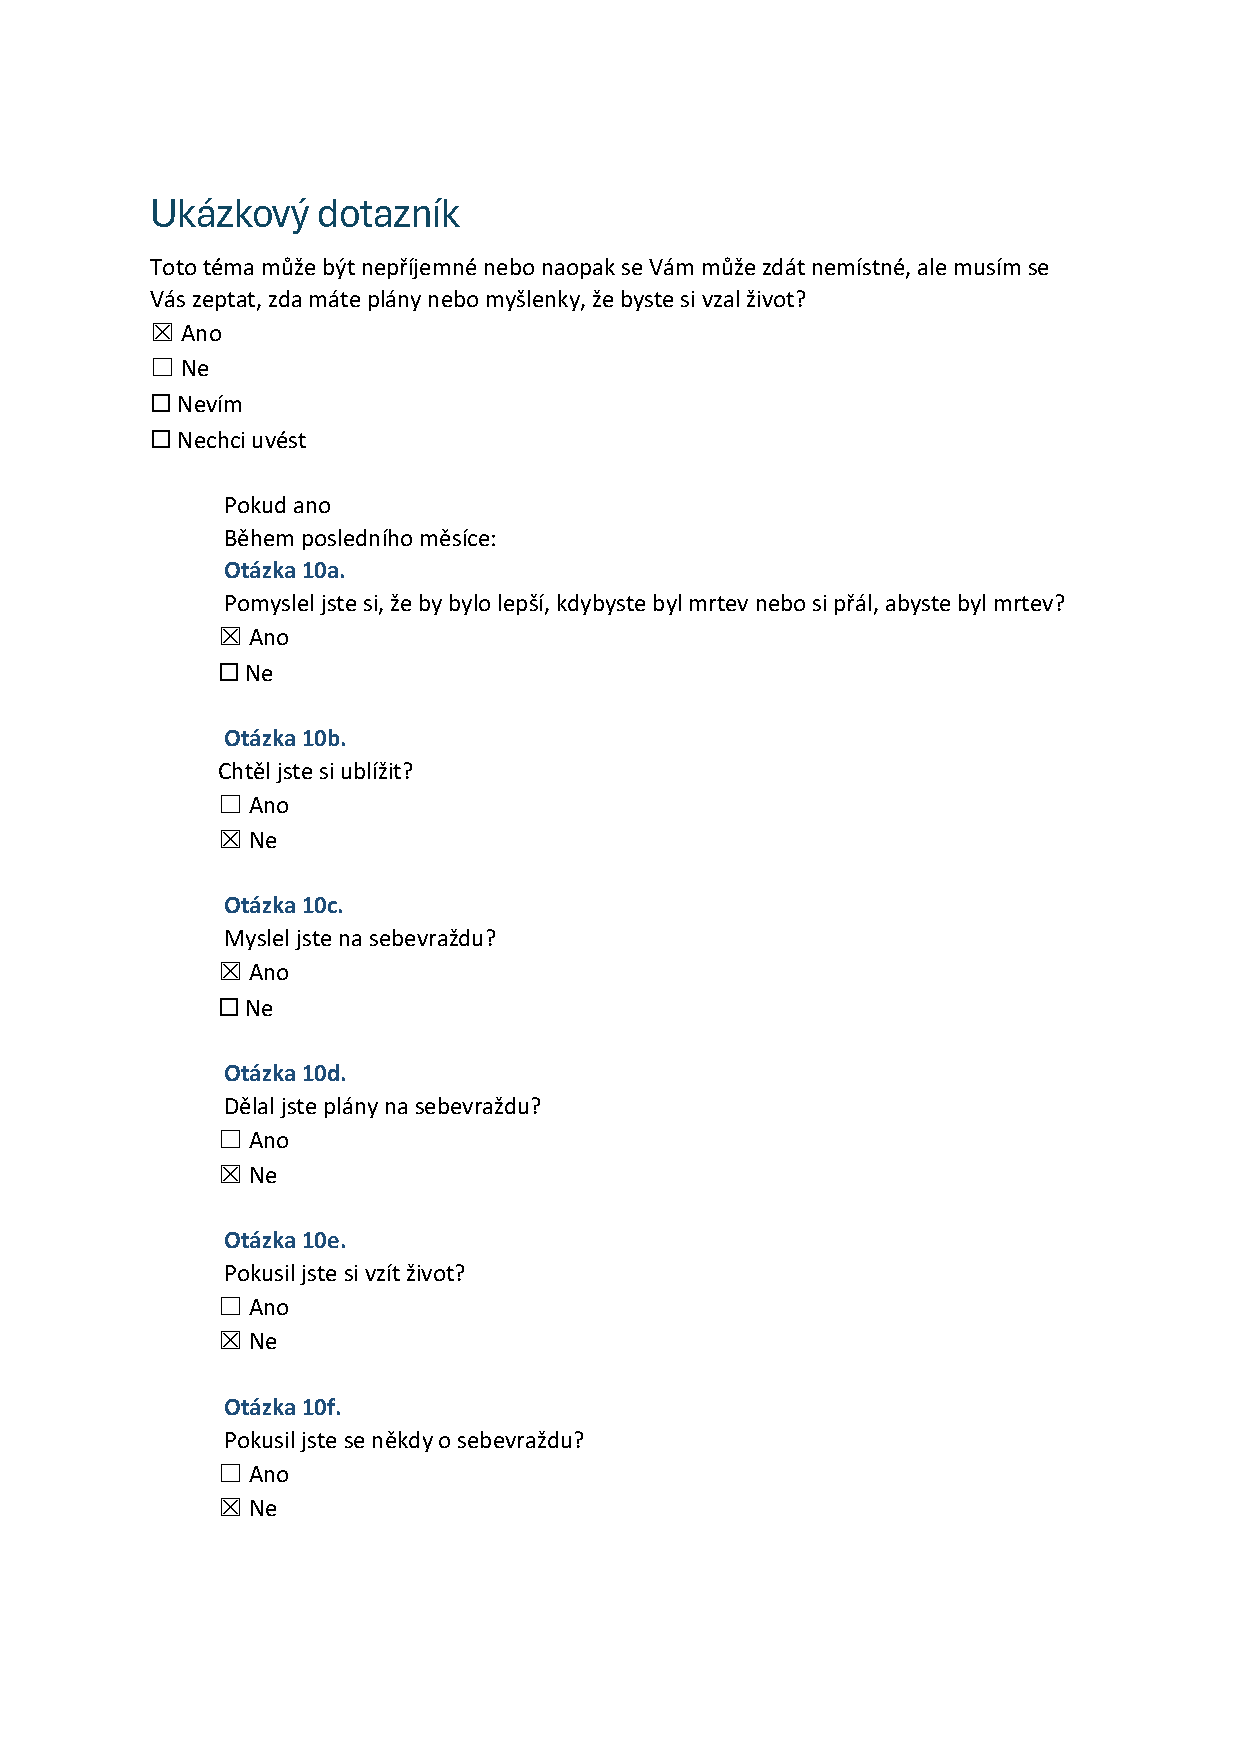
\includegraphics[width=0.8\textwidth]{../attachments/ukazkovy-dotaznik}
    \caption{Ukázkový dotazník poskytnutý zadavatelem}\label{fig:ukazkovy-dotaznik}
\end{figure}

\section{Wireframy uživatelského rozhraní}\label{sec:wireframy-uzivatelskeho-rozhrani}

\begin{figure}[H]
    \centering
    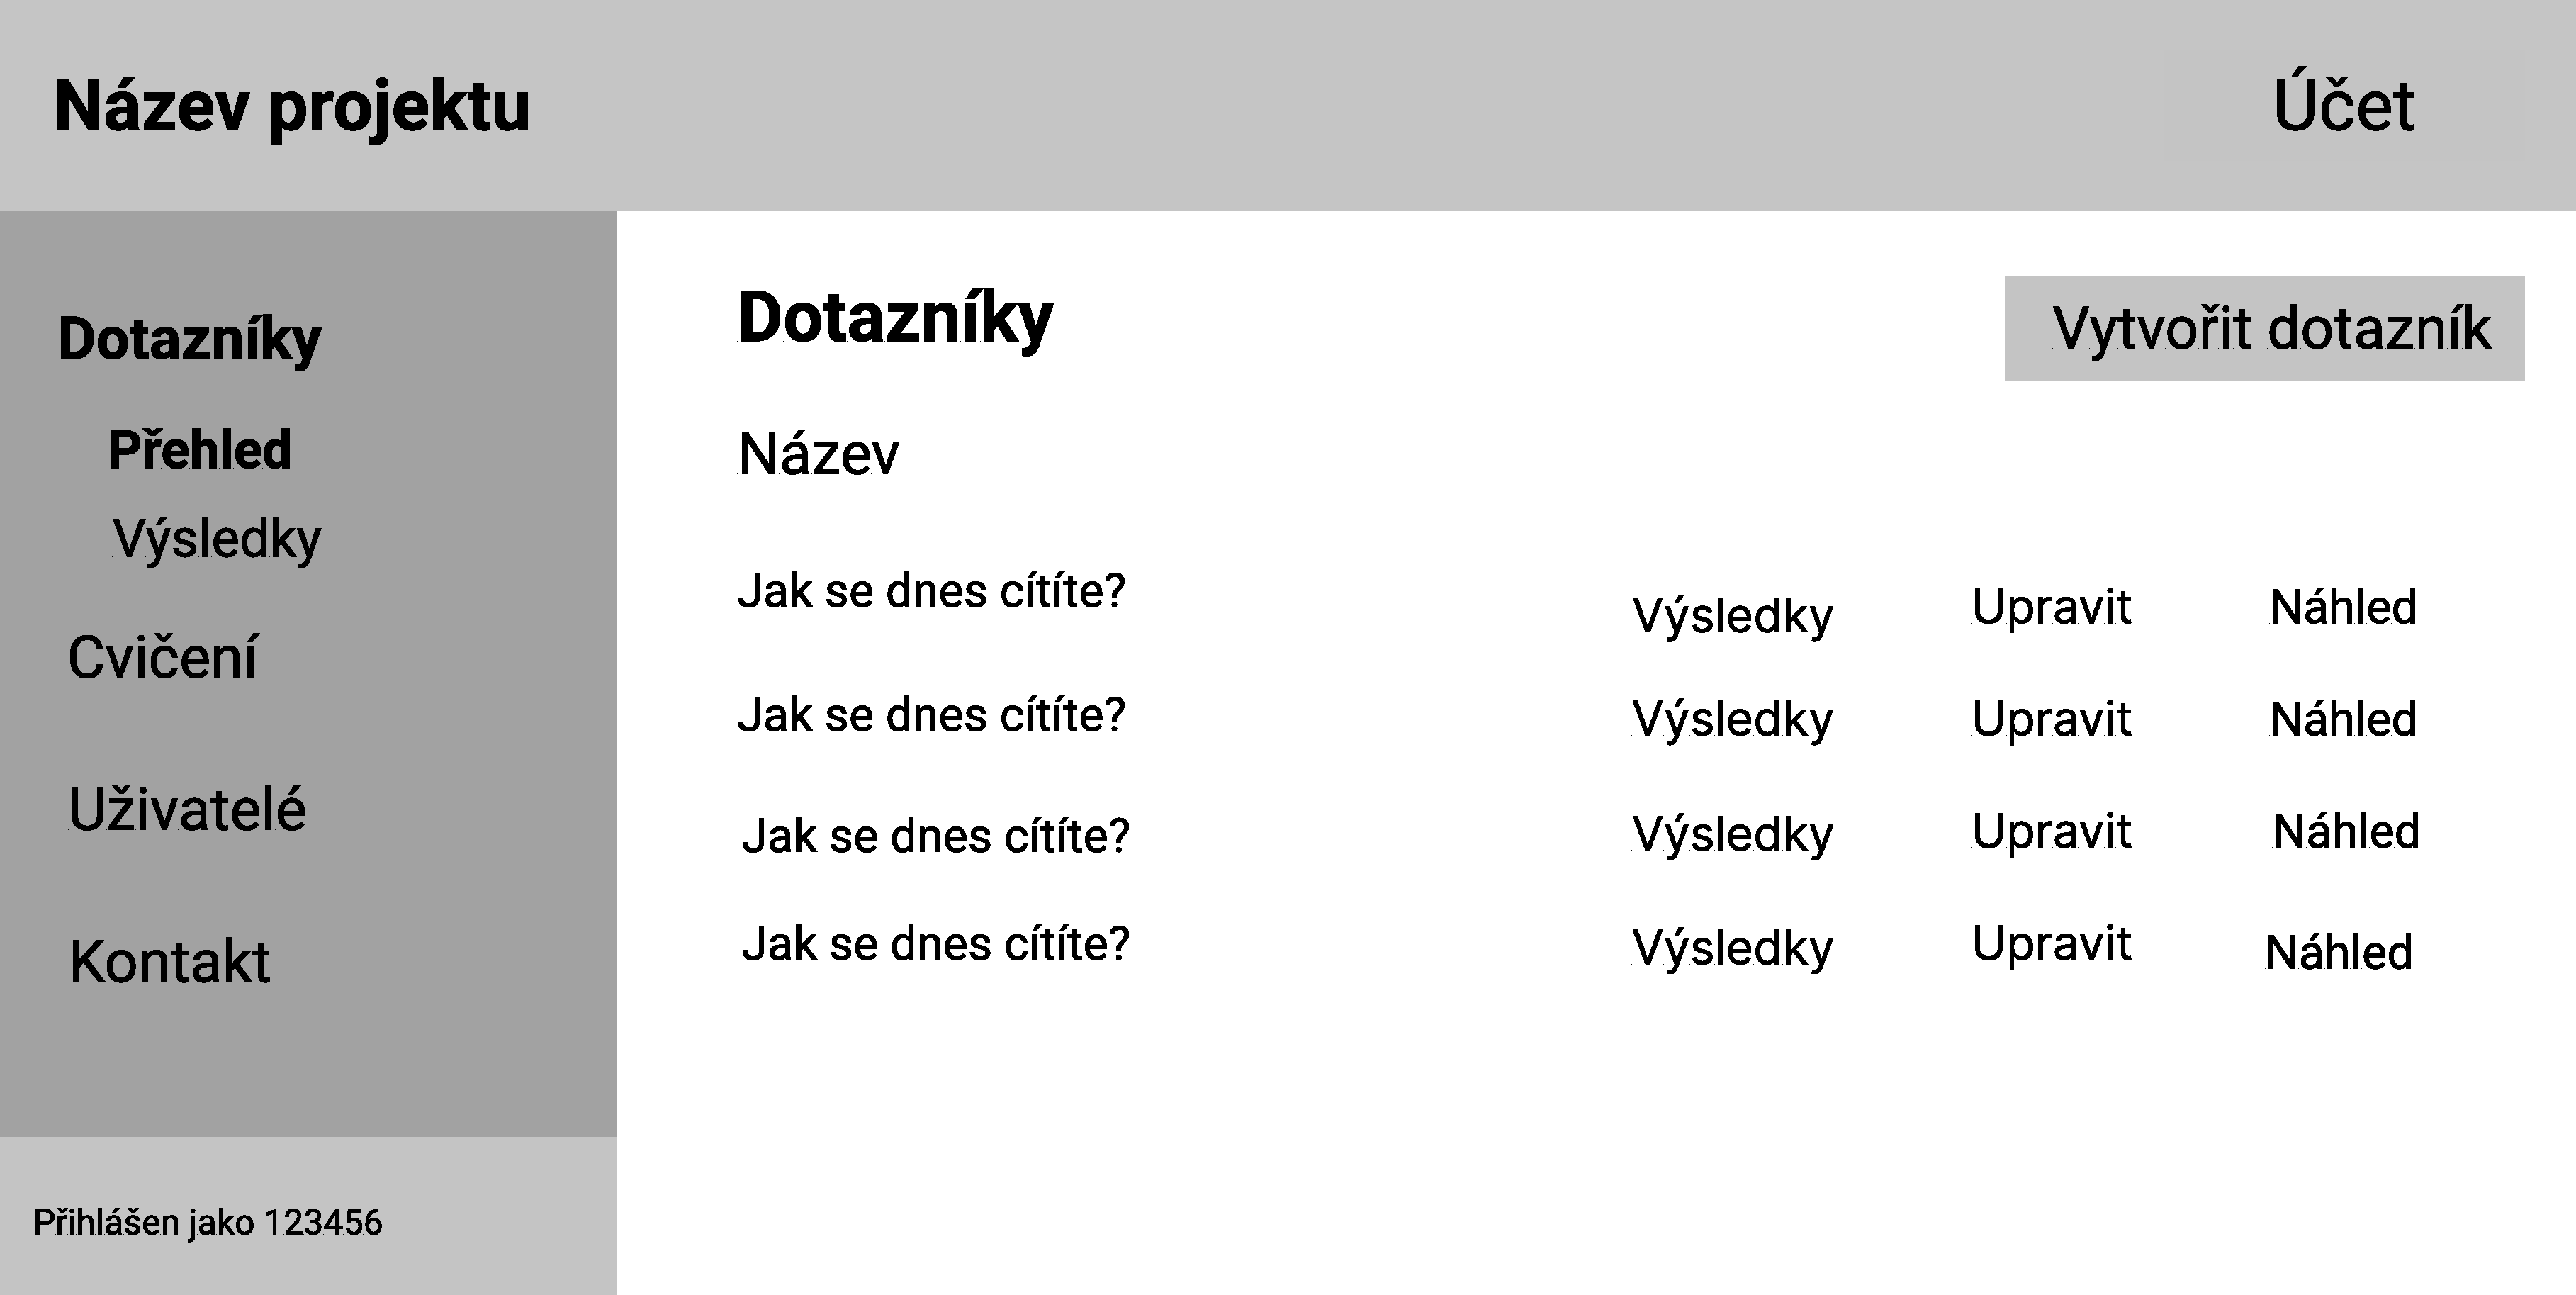
\includegraphics[width=\textwidth]{../attachments/design/zamestnanec/dotazniky-prehled}
    \caption{Přehledová stránka pro definice dotazníků pro zaměstnance}\label{fig:prehled-zamestnanec}
\end{figure}

\begin{figure}[H]
    \centering
    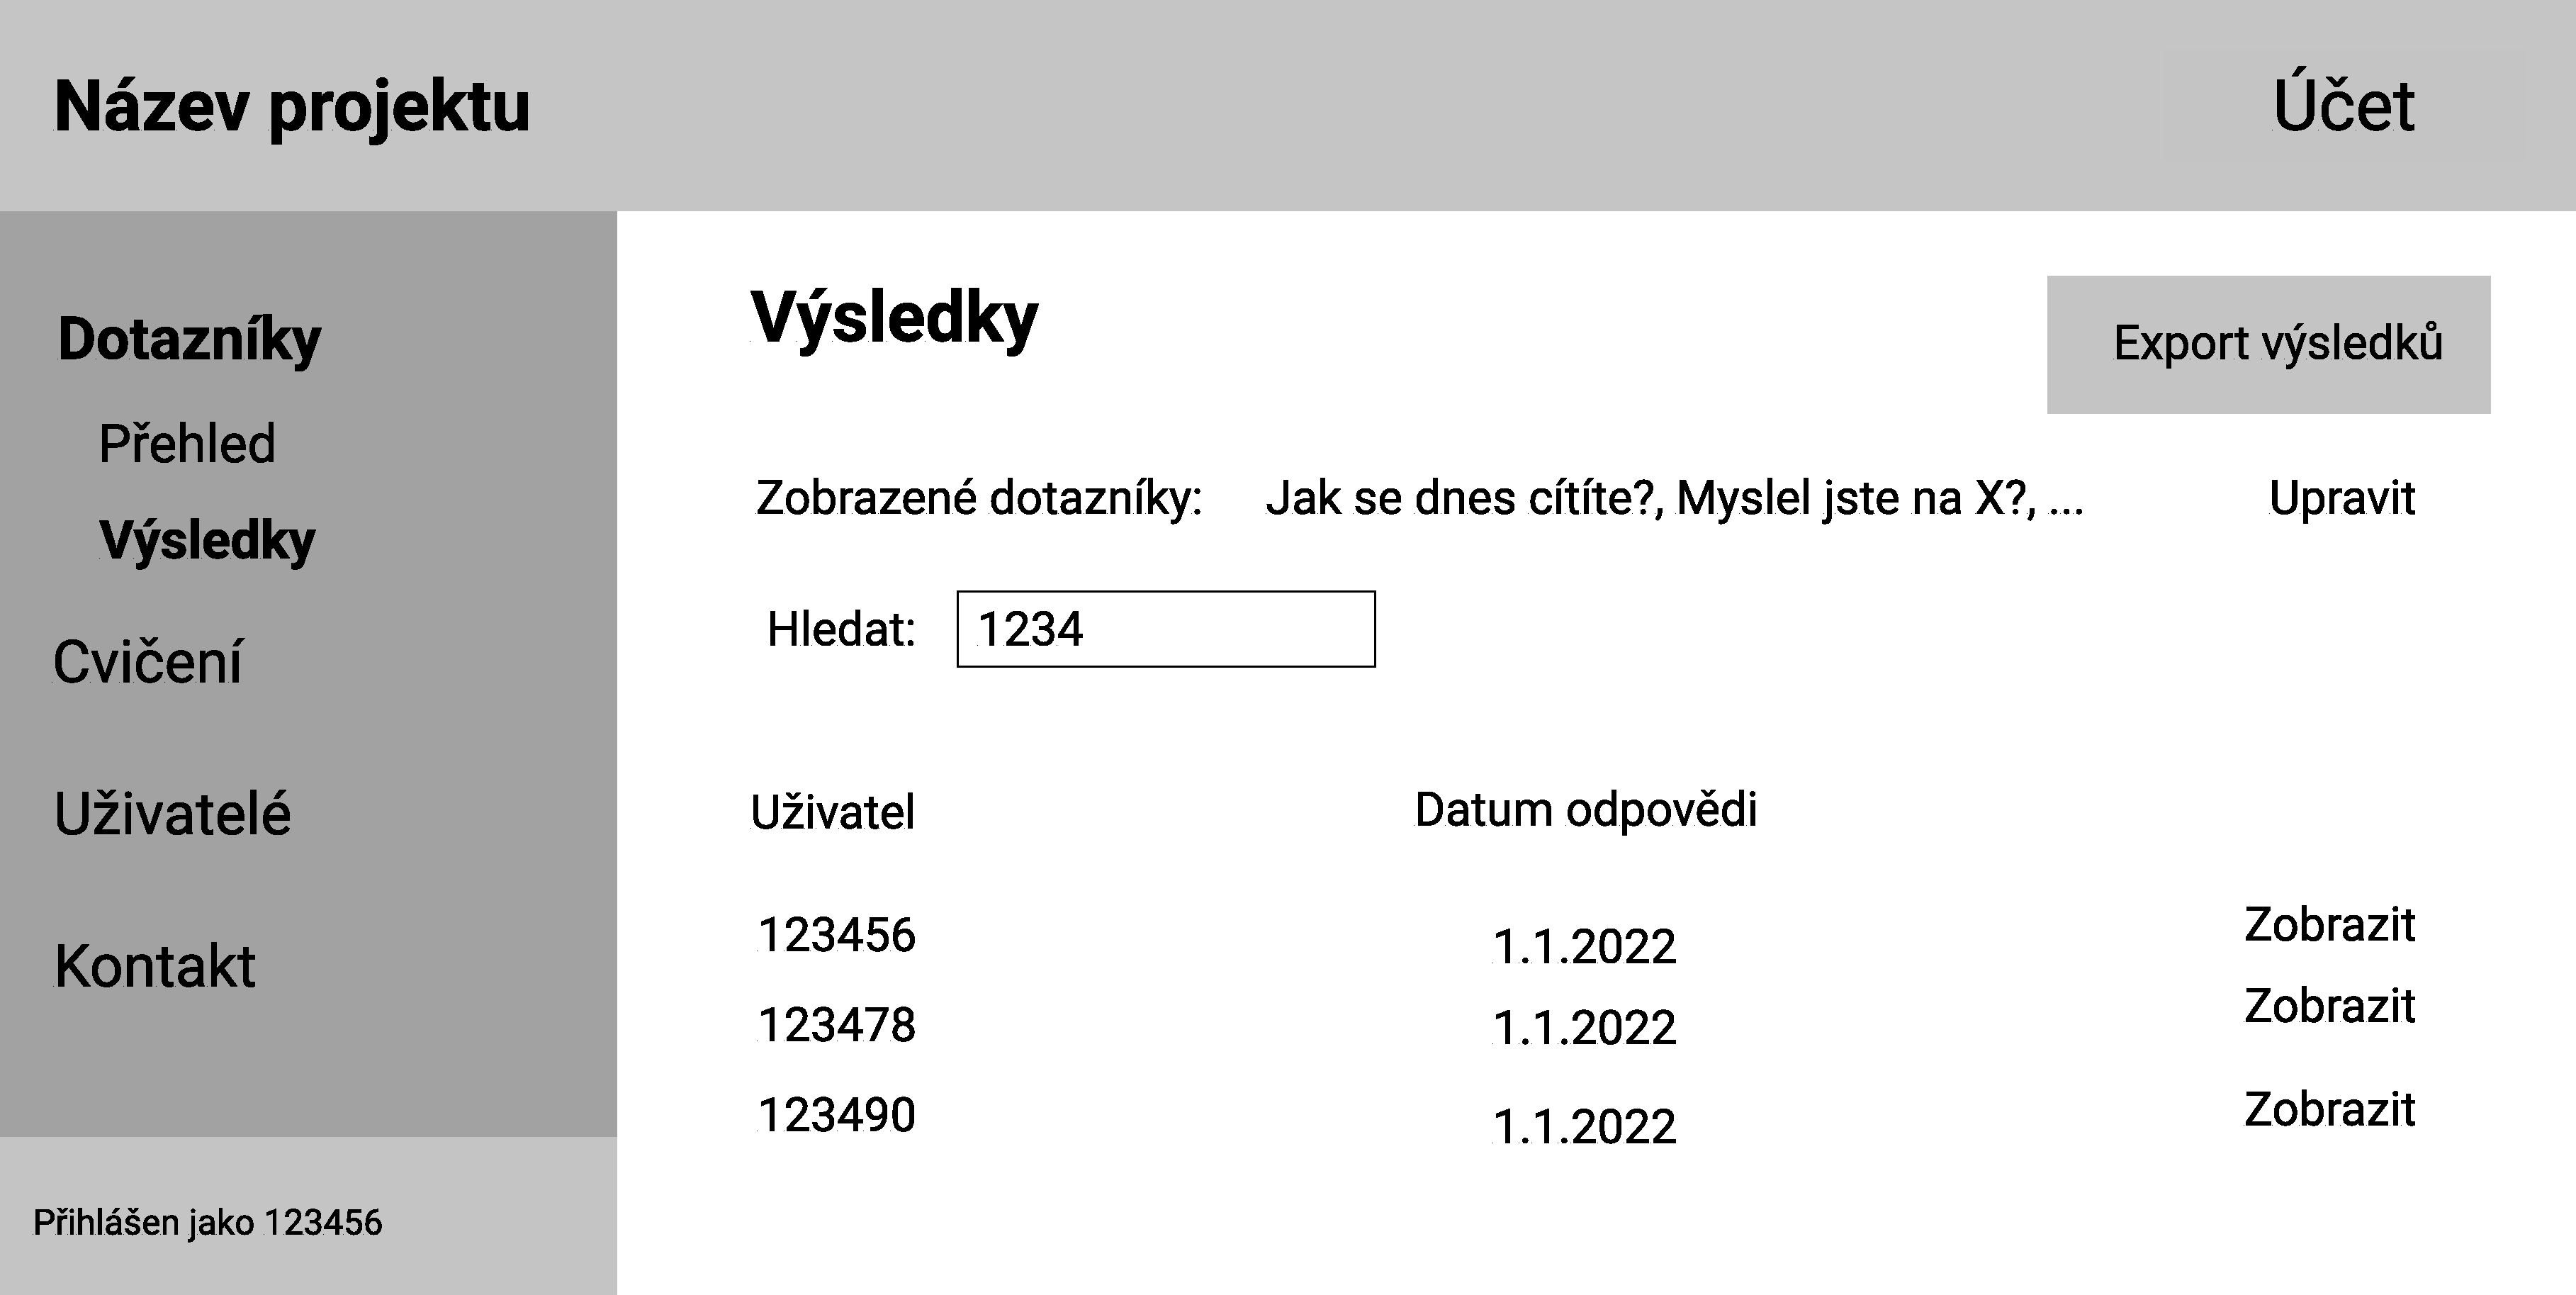
\includegraphics[width=\textwidth]{../attachments/design/zamestnanec/dotazniky-vysledky}
    \caption{Stránka s výsledky dotazníků pro zaměstnance}\label{fig:vysledky-zamestnanec}
\end{figure}

\begin{figure}[H]
    \centering
    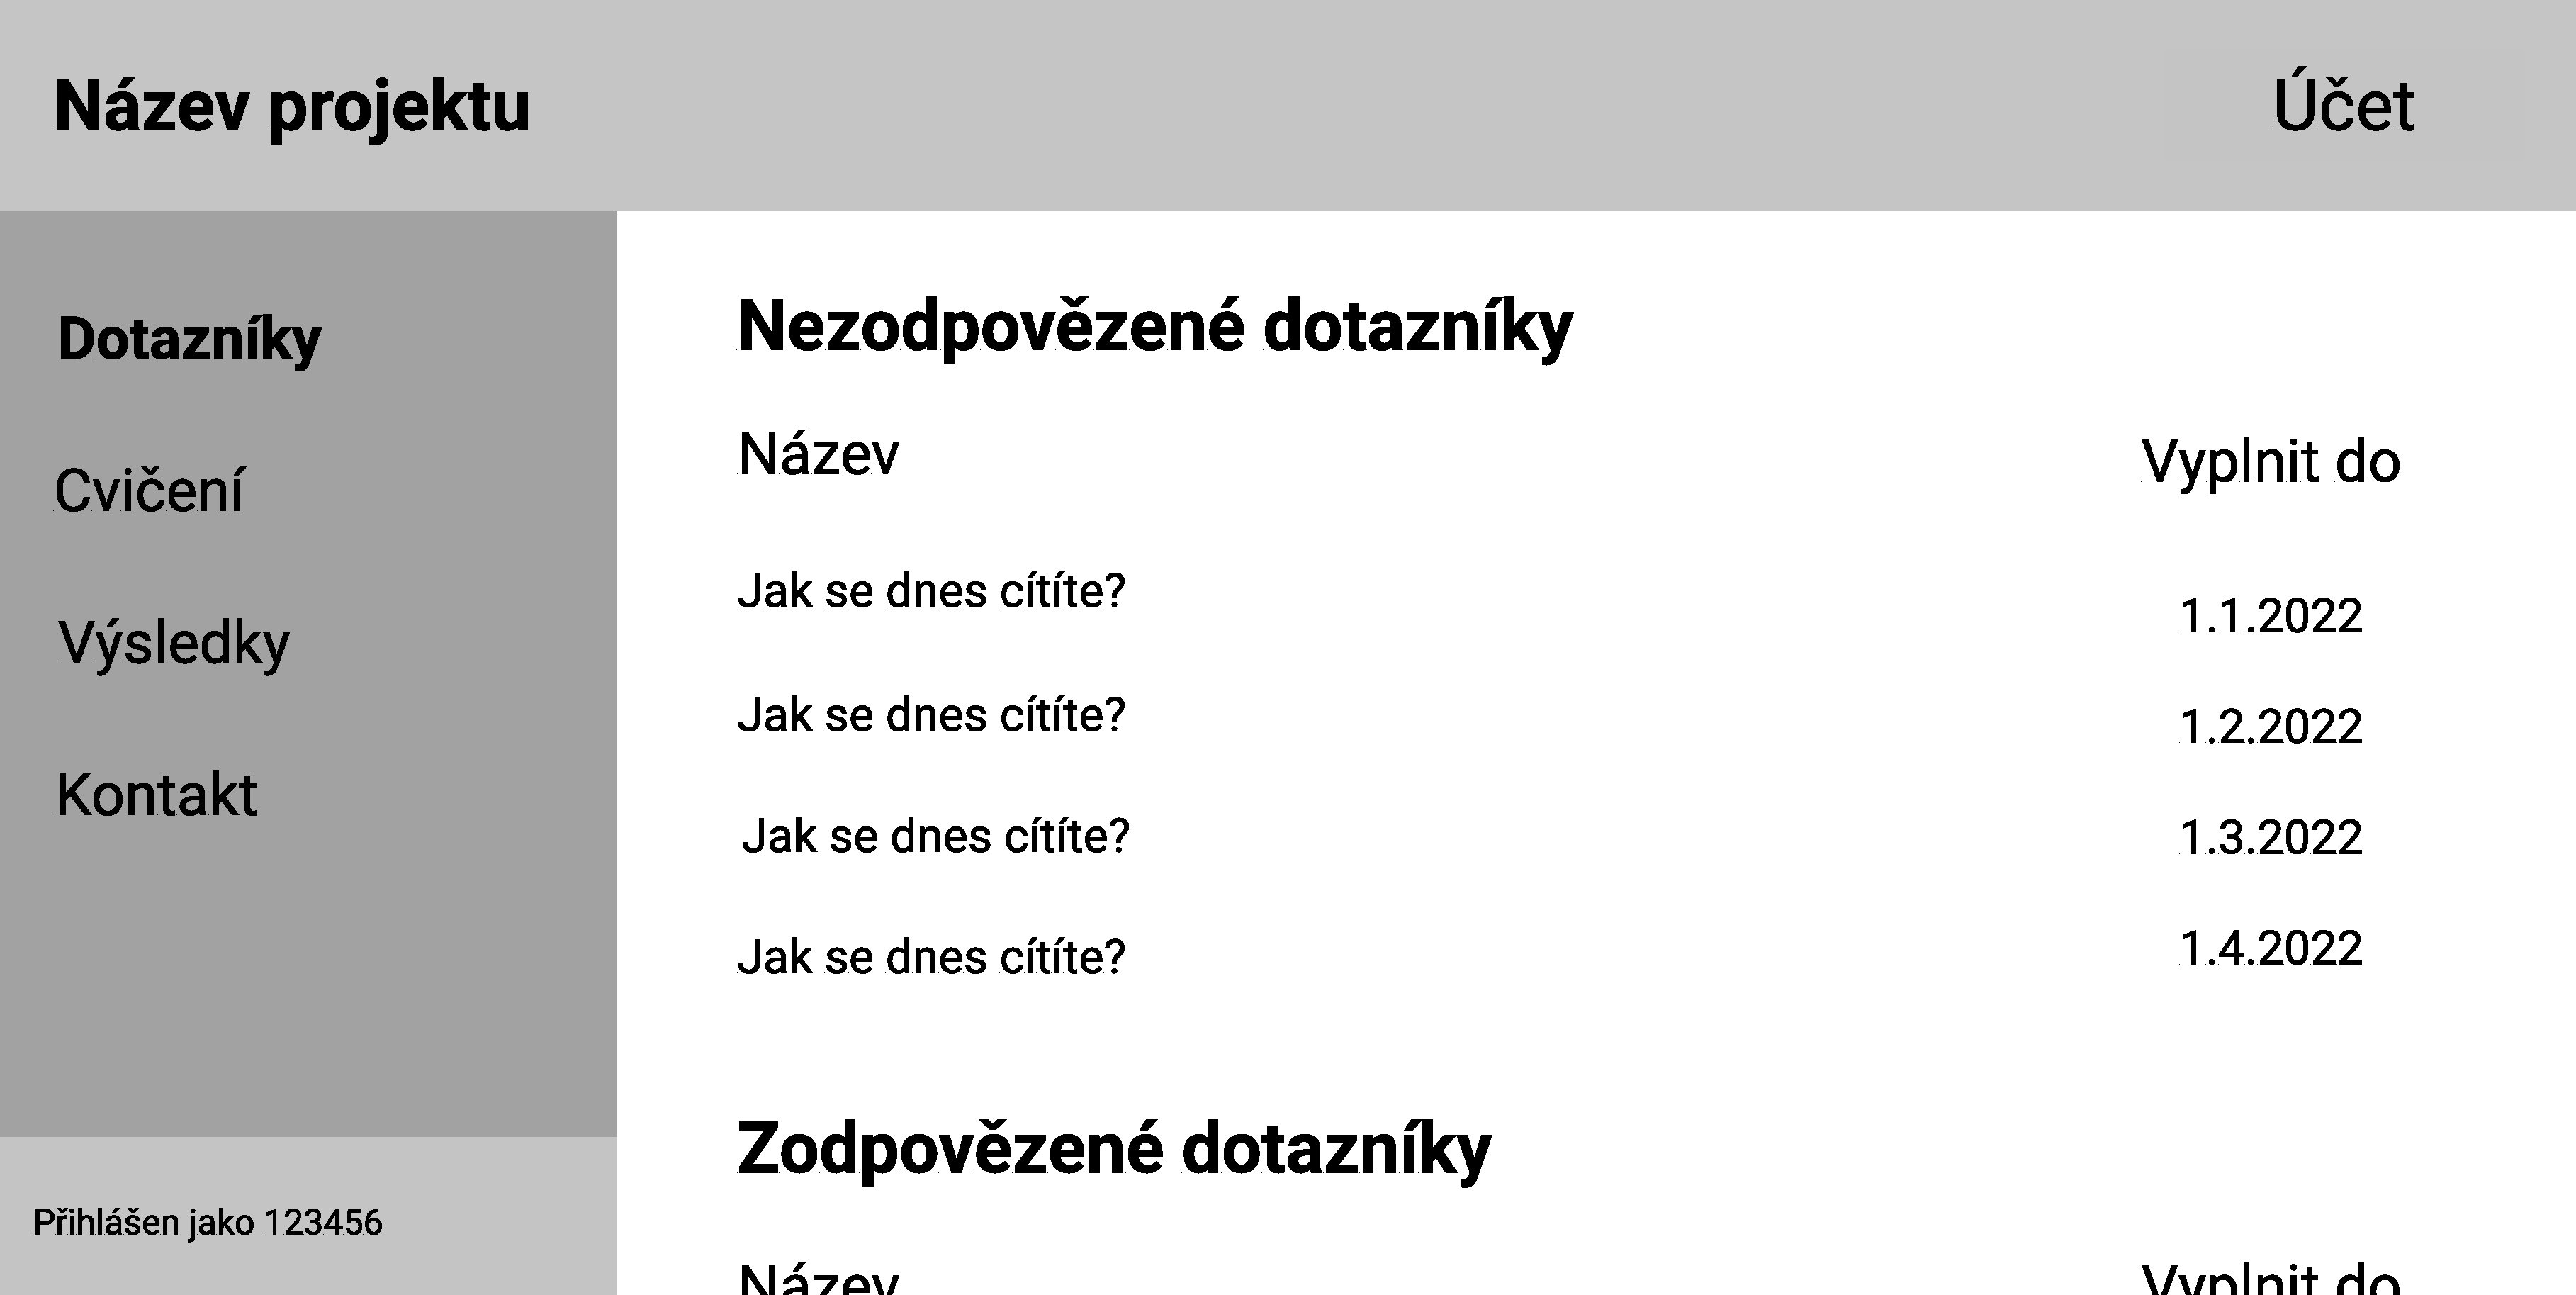
\includegraphics[width=\textwidth]{../attachments/design/uzivatel/ukoly-prehled}
    \caption{Stránka s úkoly pro uživatele}\label{fig:ukoly-prehled}
\end{figure}

\openright
\end{document}
